\documentclass[12pt]{extarticle}
\usepackage[paperwidth=15in,paperheight=6in]{geometry}
\usepackage{amsmath}
\usepackage{hyperref}
\usepackage{pdfpages}
\usepackage[utf8]{inputenc}
\title{Kaon mixing: chiral and continuum extrapolations}
\author{R Mukherjee}
\date{\today}
\begin{document}
\maketitle
\tableofcontents
\clearpage
\section{VVpAA}
\begin{table}[!h]
\begin{center}
\begin{tabular*}{\linewidth}{@{\extracolsep{\fill}} |c|c|c|c|c|}
\hline
$\mu$ (GeV) & $a^2$, $m_\pi^2$ & $a^2$, $m_\pi^2$ no C & $a^2$, $a^4$, $m_\pi^2$ & $a^2$, $m_\pi^2$, $m_\pi^4$\\
\hline
2.0& \hyperlink{VVpAA/a2m2_20.pdf.1}{\textbf{0.5264(11)}: 1.838 (0.102)} & \hyperlink{VVpAA/a2m2noC_20.pdf.1}{\textbf{0.5310(48)}: 0.864 (0.421)} & \hyperlink{VVpAA/a2a4m2_20.pdf.1}{\textbf{0.5326(82)}: 2.159 (0.071)} & \hyperlink{VVpAA/a2m2m4_20.pdf.1}{\textbf{0.5282(12)}: 0.639 (0.635)}\\
1.8& \hyperlink{VVpAA/a2m2_18.pdf.1}{\textbf{0.5293(14)}: 1.315 (0.254)} & \hyperlink{VVpAA/a2m2noC_18.pdf.1}{\textbf{0.5328(53)}: 0.478 (0.62)} & \hyperlink{VVpAA/a2a4m2_18.pdf.1}{\textbf{0.5335(91)}: 1.6 (0.171)} & \hyperlink{VVpAA/a2m2m4_18.pdf.1}{\textbf{0.5310(14)}: 0.307 (0.873)}\\
1.5& \hyperlink{VVpAA/a2m2_15.pdf.1}{\textbf{0.5338(19)}: 0.734 (0.598)} & \hyperlink{VVpAA/a2m2noC_15.pdf.1}{\textbf{0.5356(64)}: 0.159 (0.853)} & \hyperlink{VVpAA/a2a4m2_15.pdf.1}{\textbf{0.536(11)}: 0.909 (0.457)} & \hyperlink{VVpAA/a2m2m4_15.pdf.1}{\textbf{0.5352(18)}: 0.099 (0.983)}\\
\hline
\end{tabular*}
\caption{Physical point value from chiral and continuum extrapolation at renormalisation scale $\mu$. Entries are \textbf{value(error)}: $\chi^2/\text{DOF}$ ($p$-value).}
\end{center}
\end{table}
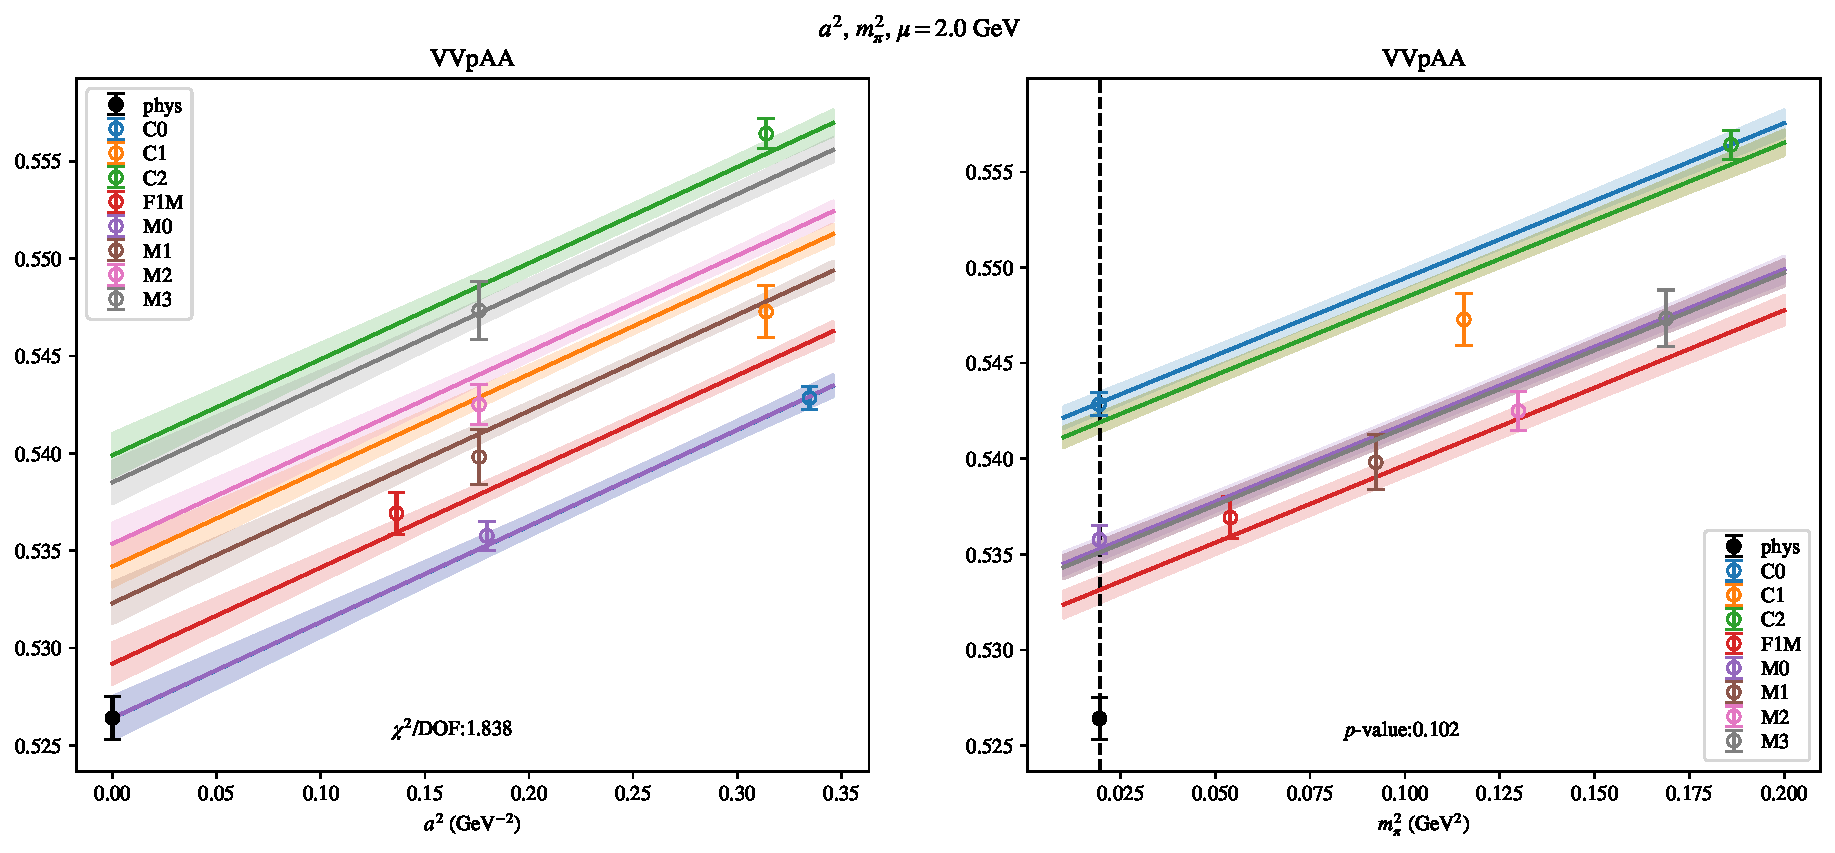
\includepdf[link, pages=-]{VVpAA/a2m2_20.pdf}
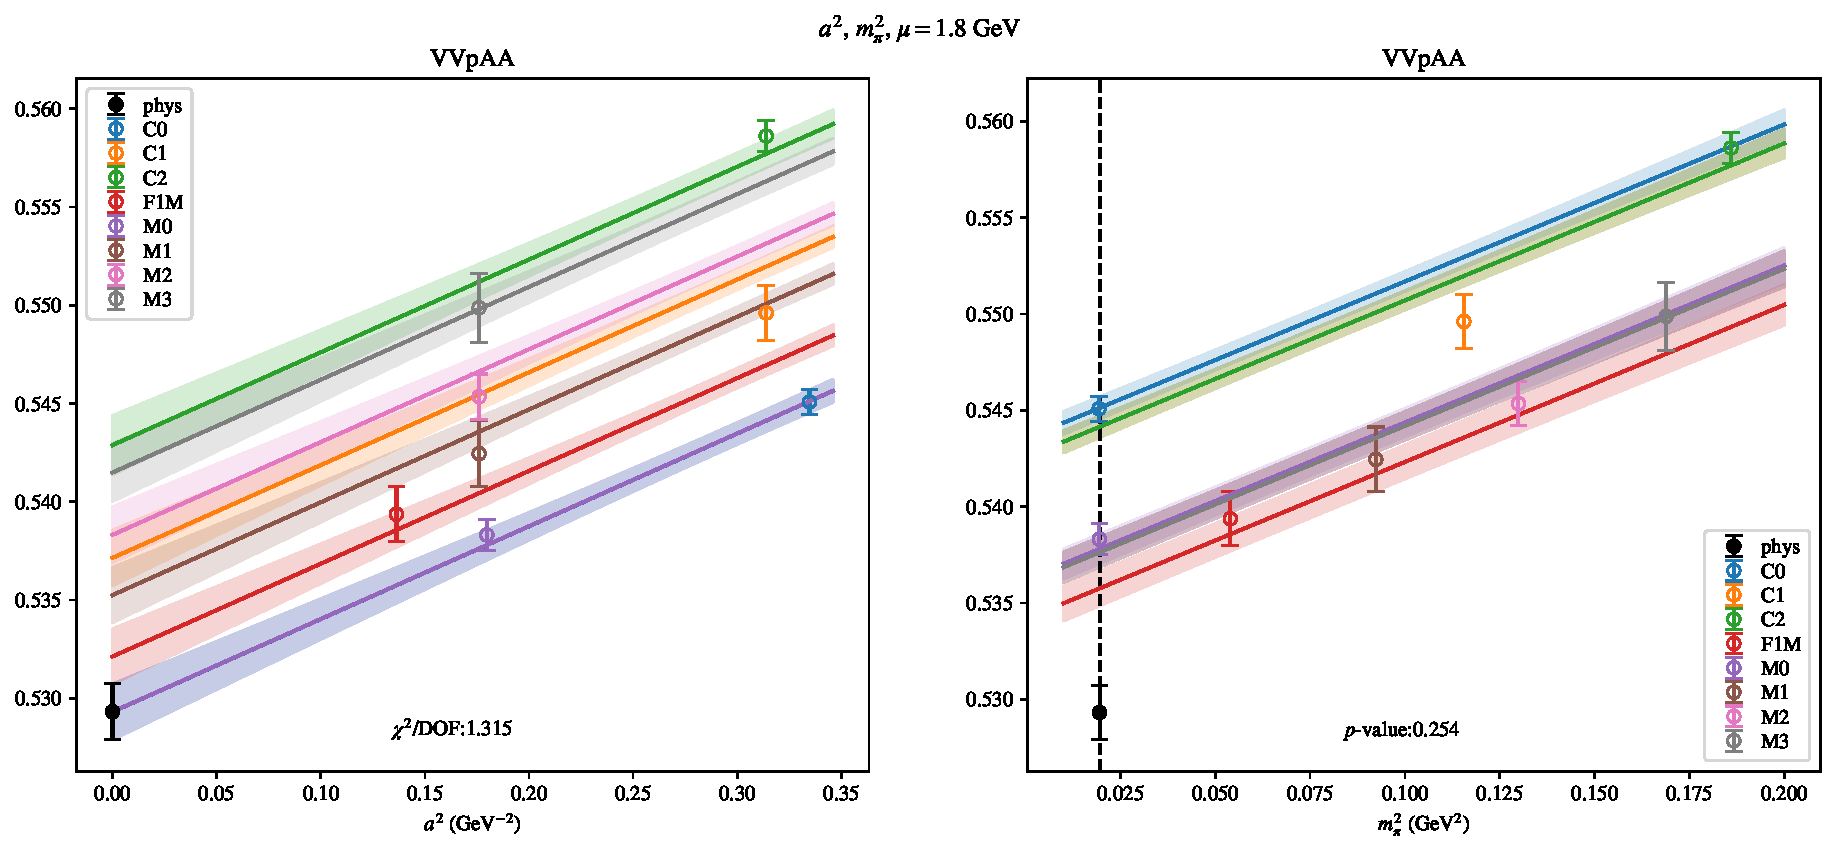
\includepdf[link, pages=-]{VVpAA/a2m2_18.pdf}
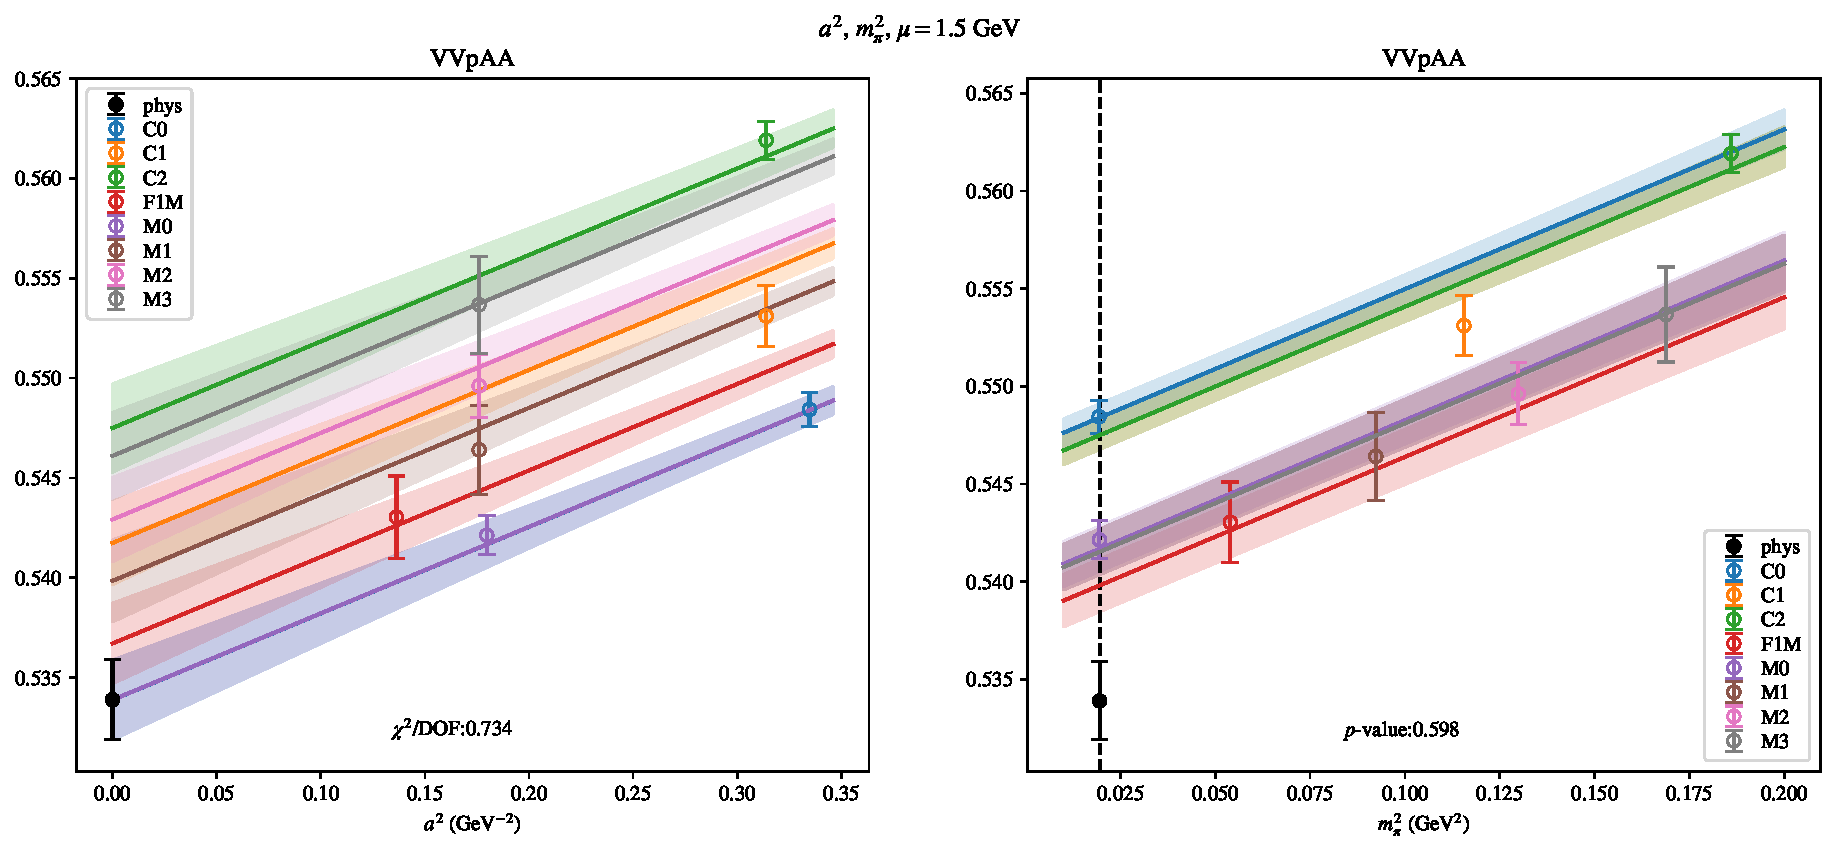
\includepdf[link, pages=-]{VVpAA/a2m2_15.pdf}
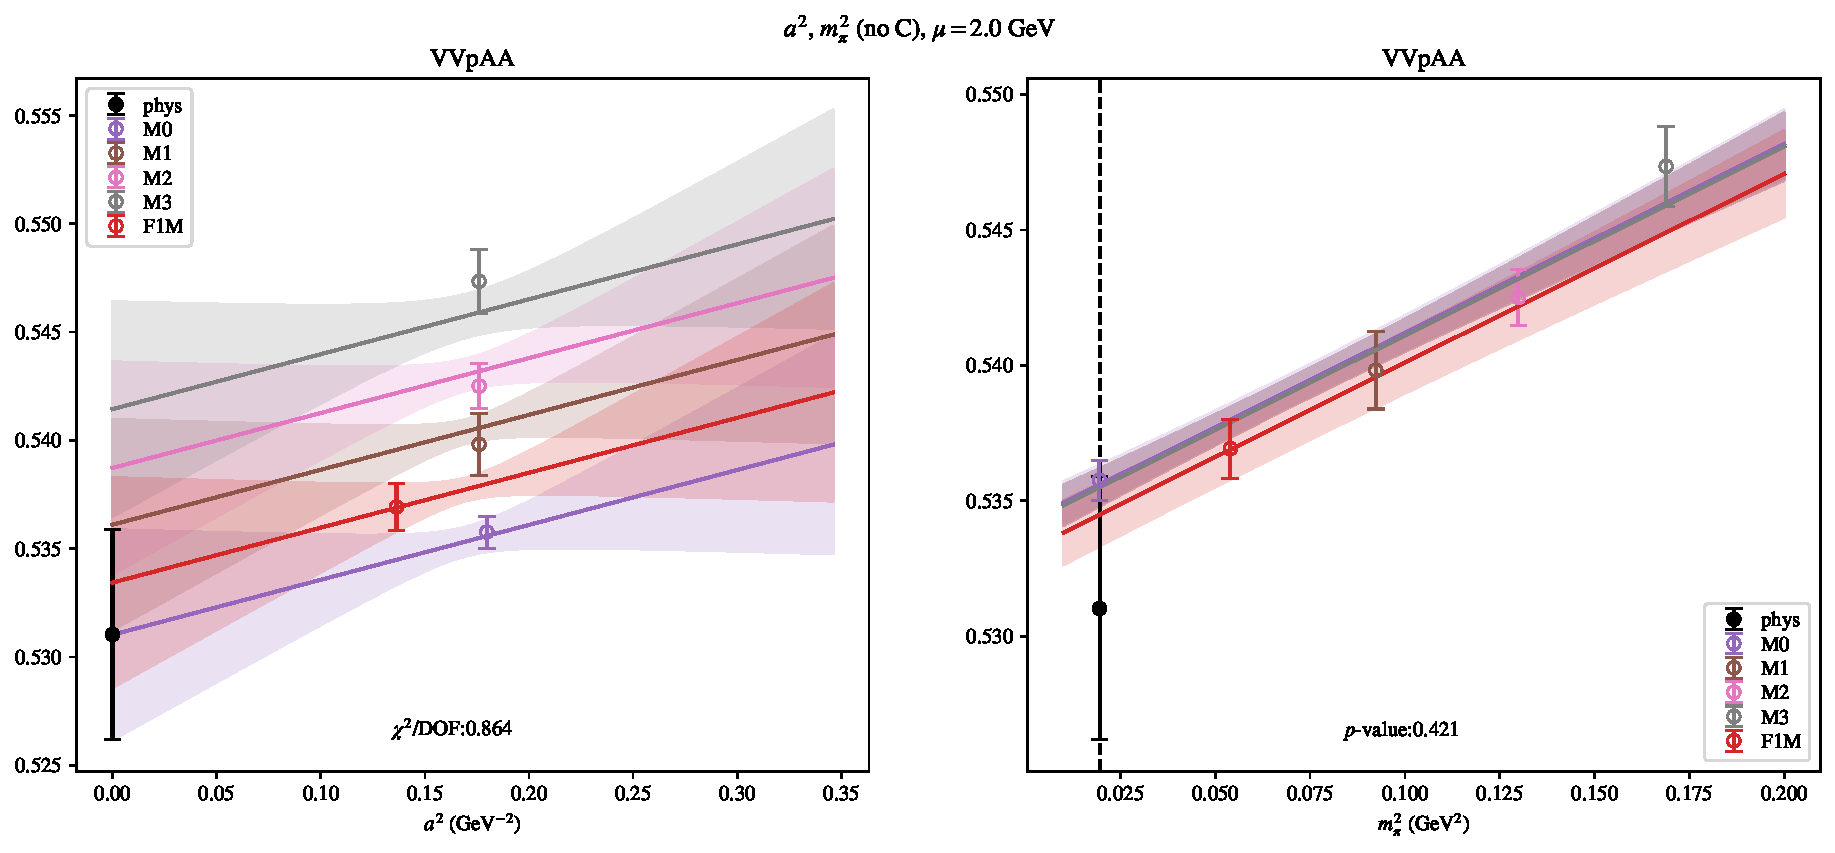
\includepdf[link, pages=-]{VVpAA/a2m2noC_20.pdf}
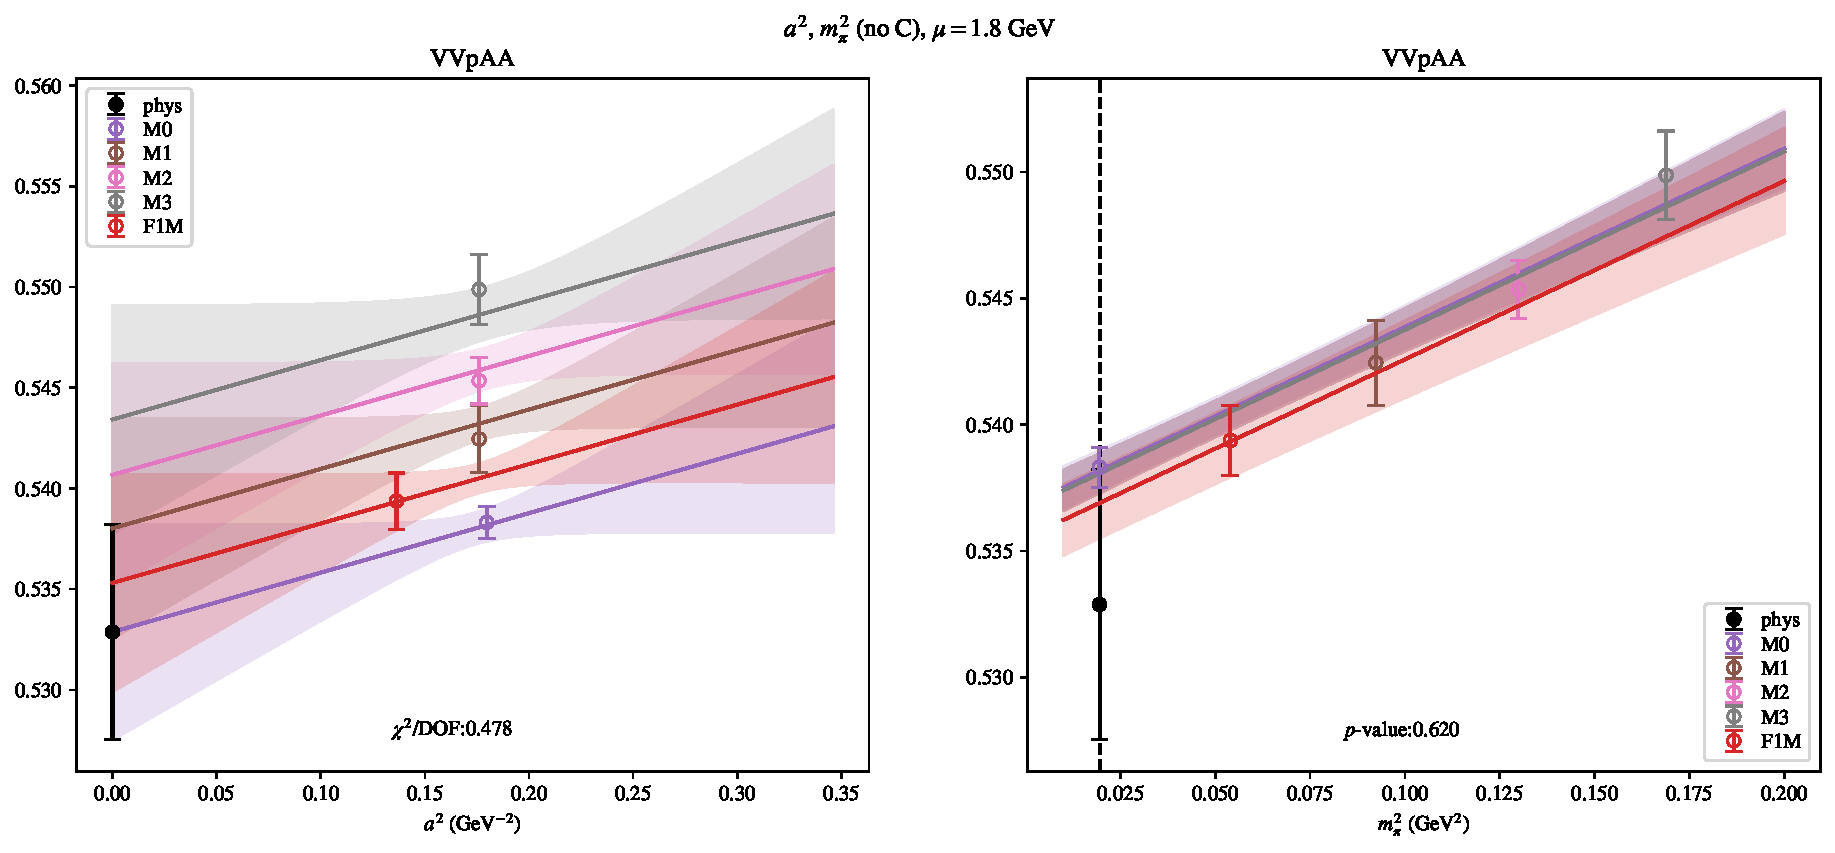
\includepdf[link, pages=-]{VVpAA/a2m2noC_18.pdf}
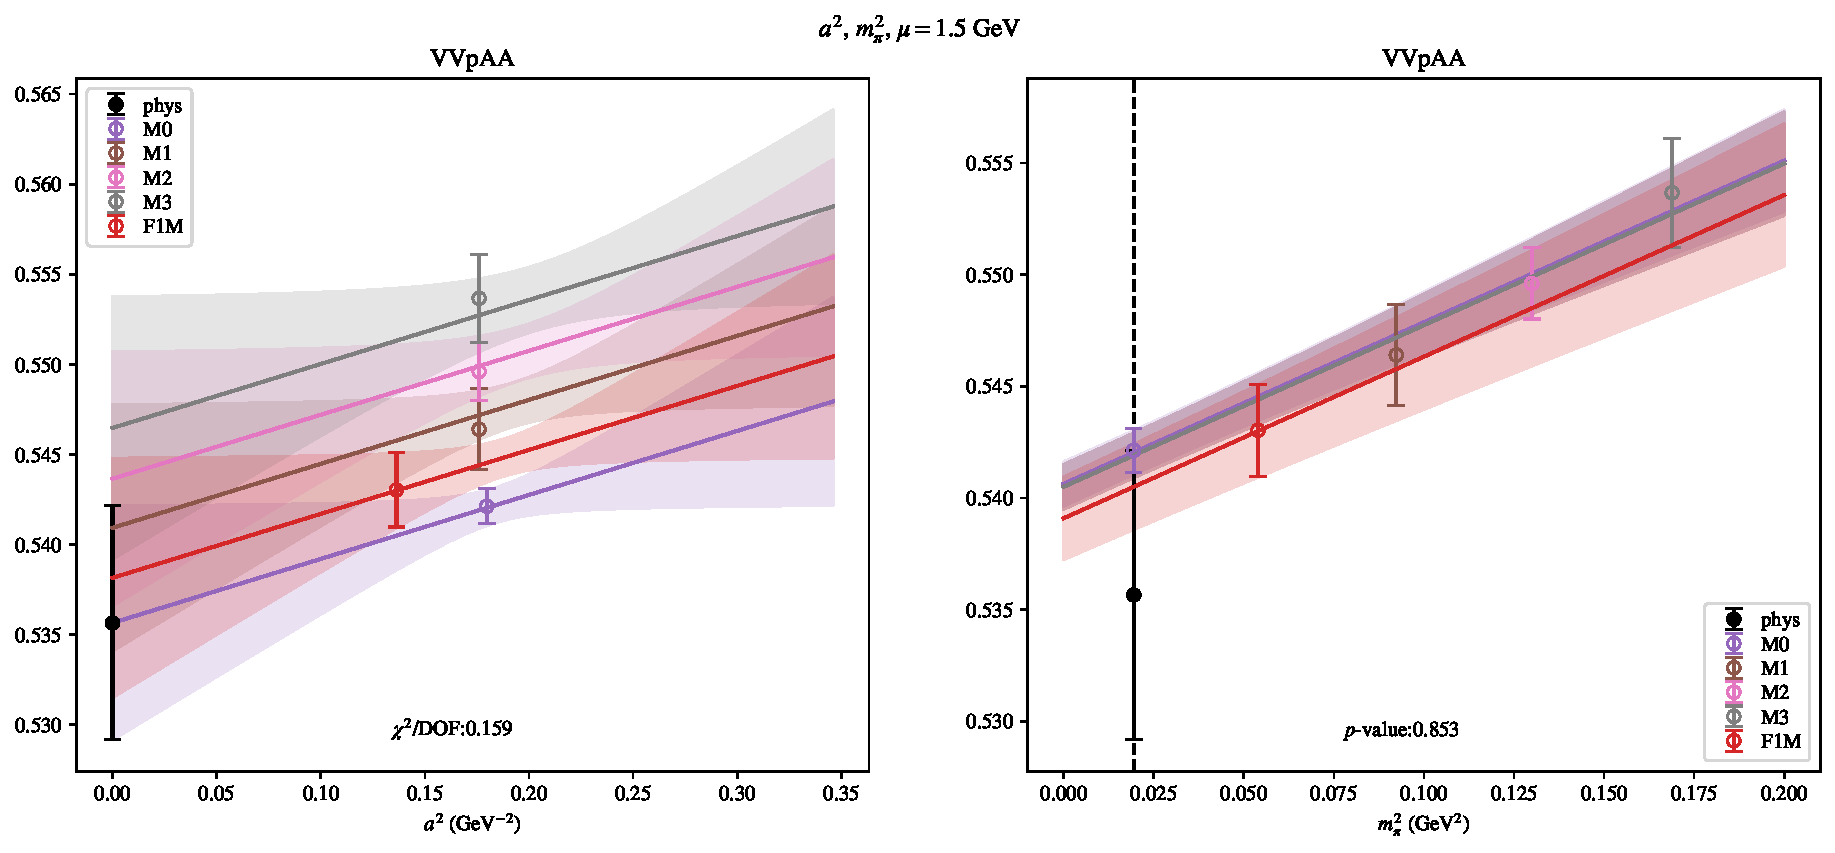
\includepdf[link, pages=-]{VVpAA/a2m2noC_15.pdf}
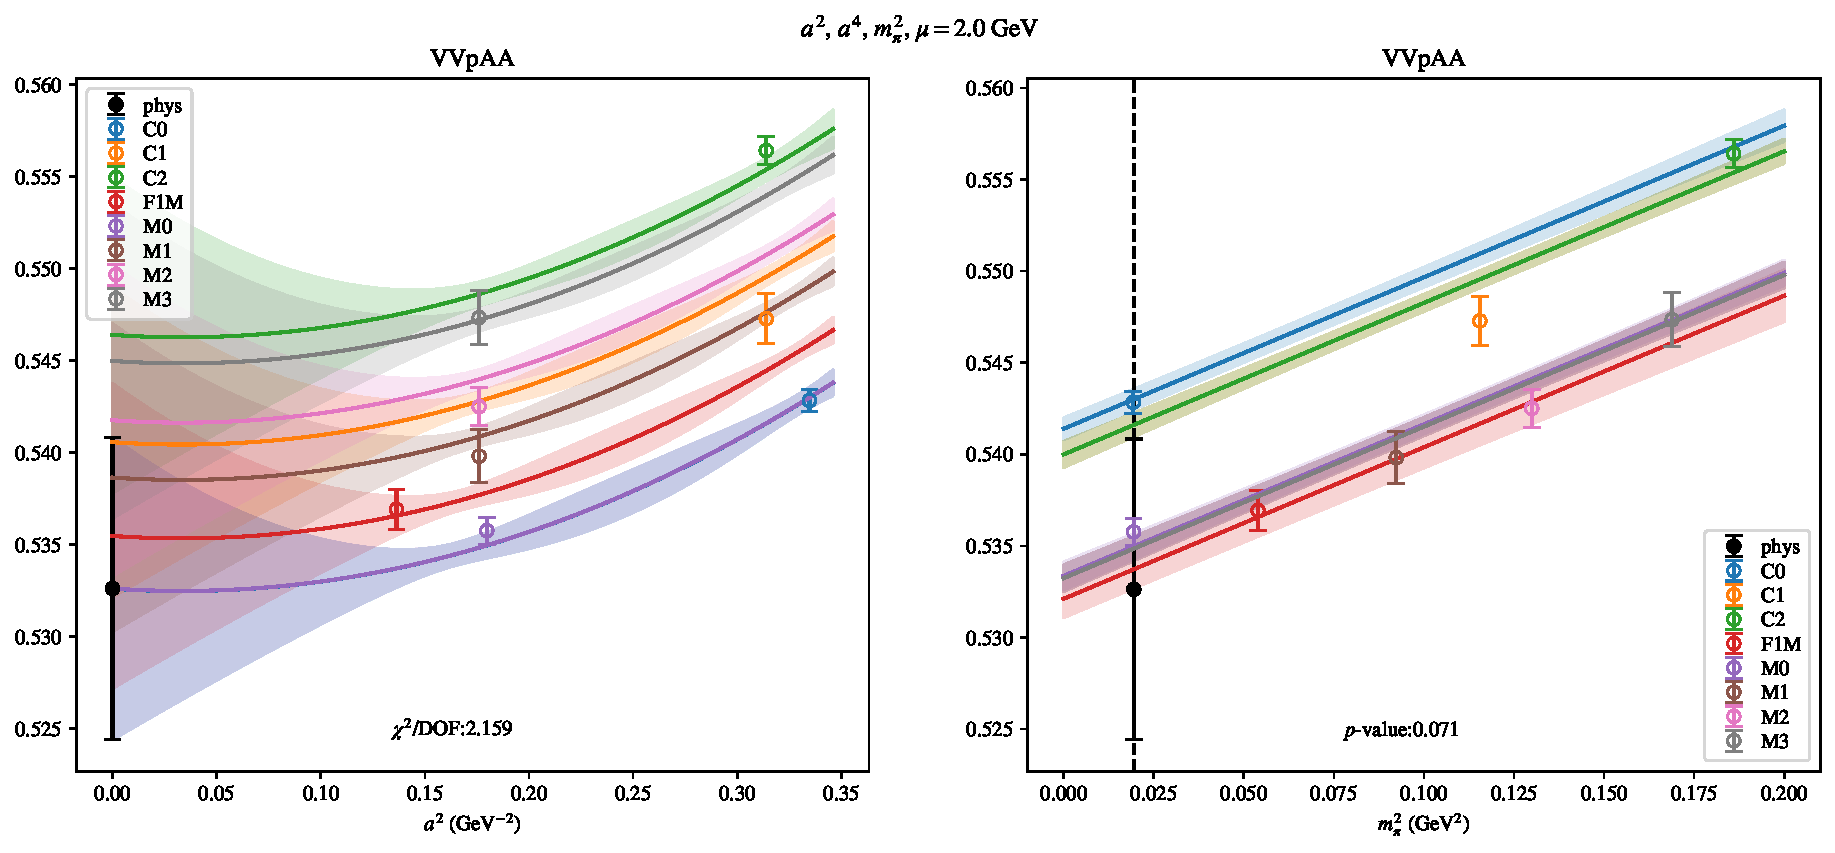
\includepdf[link, pages=-]{VVpAA/a2a4m2_20.pdf}
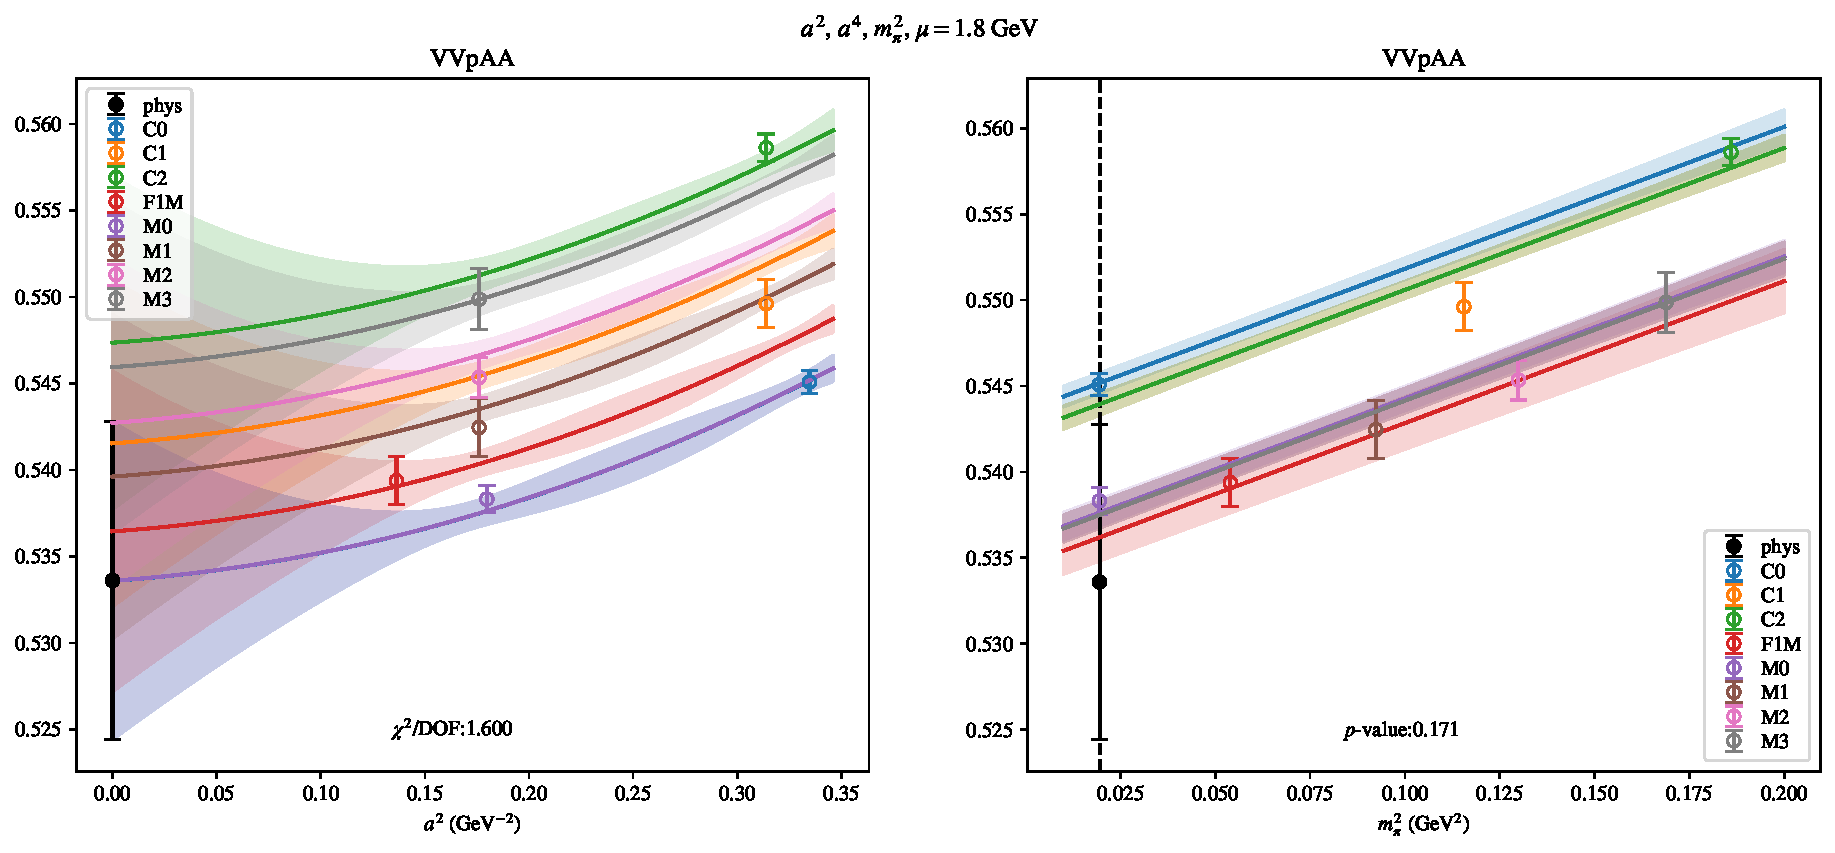
\includepdf[link, pages=-]{VVpAA/a2a4m2_18.pdf}
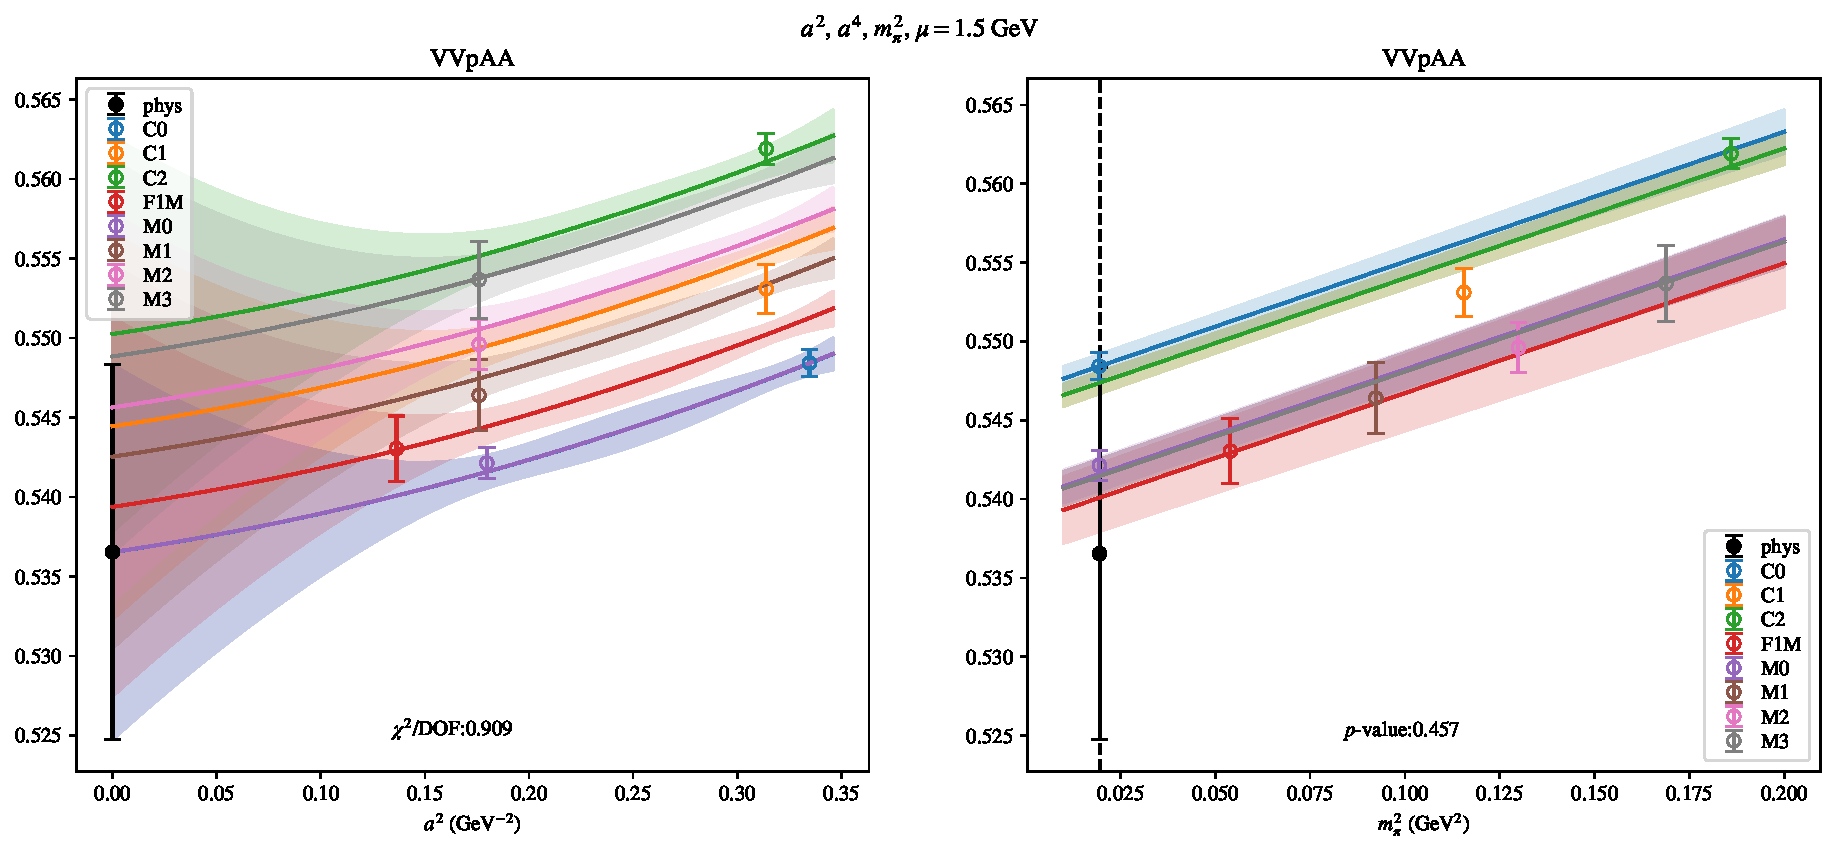
\includepdf[link, pages=-]{VVpAA/a2a4m2_15.pdf}
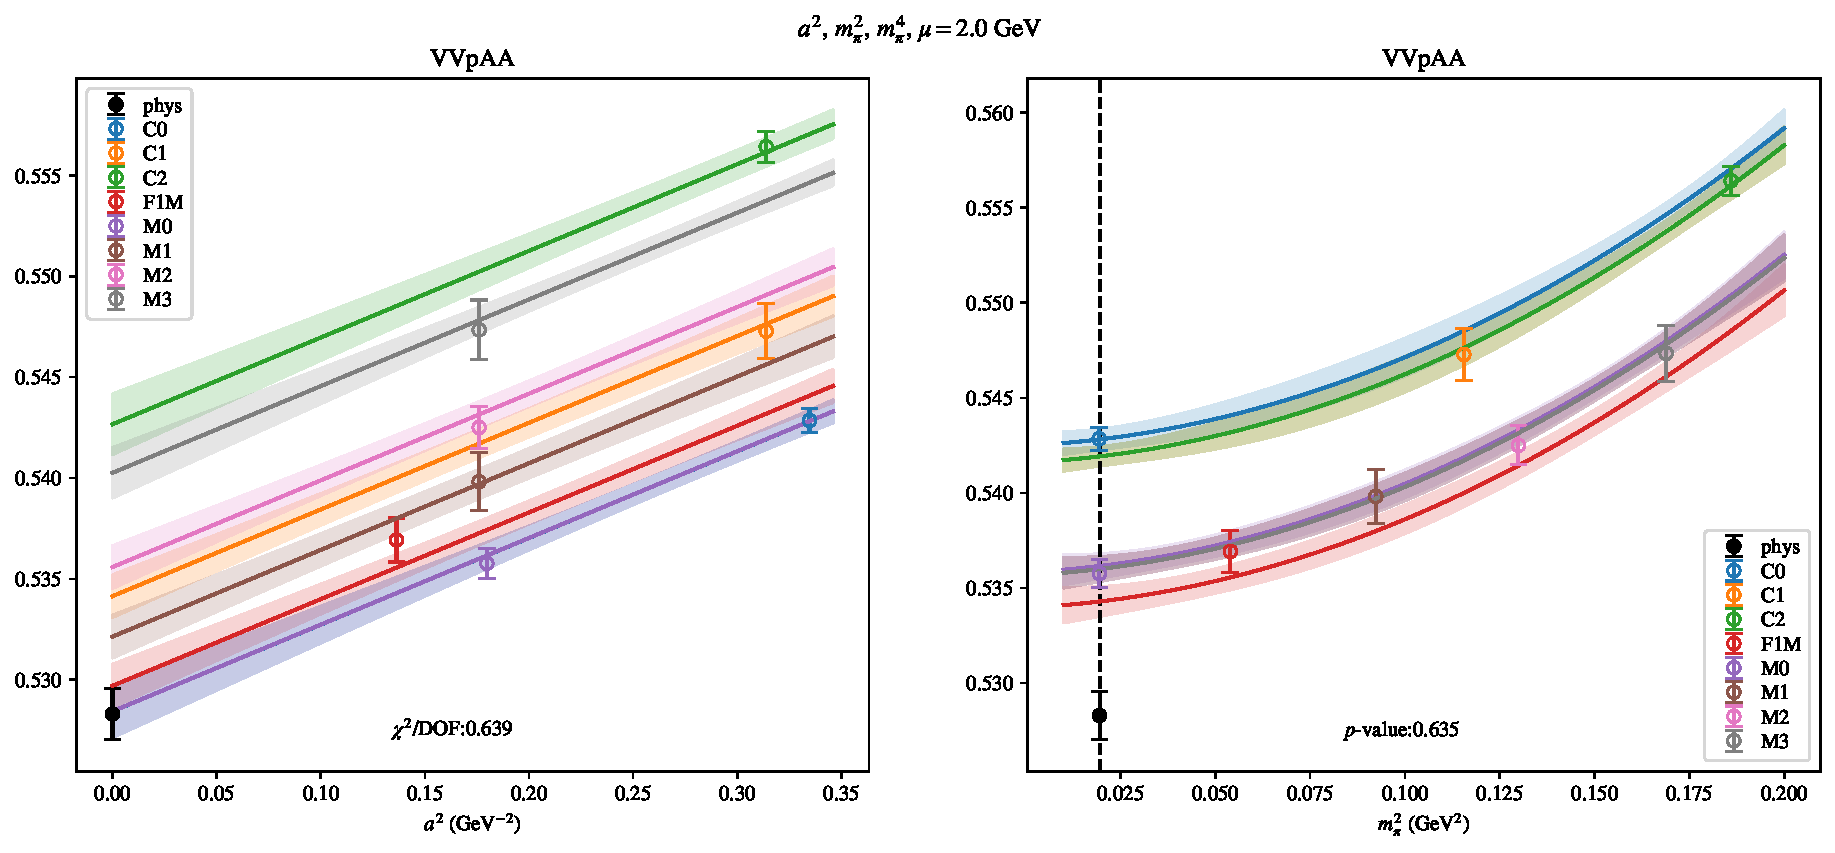
\includepdf[link, pages=-]{VVpAA/a2m2m4_20.pdf}
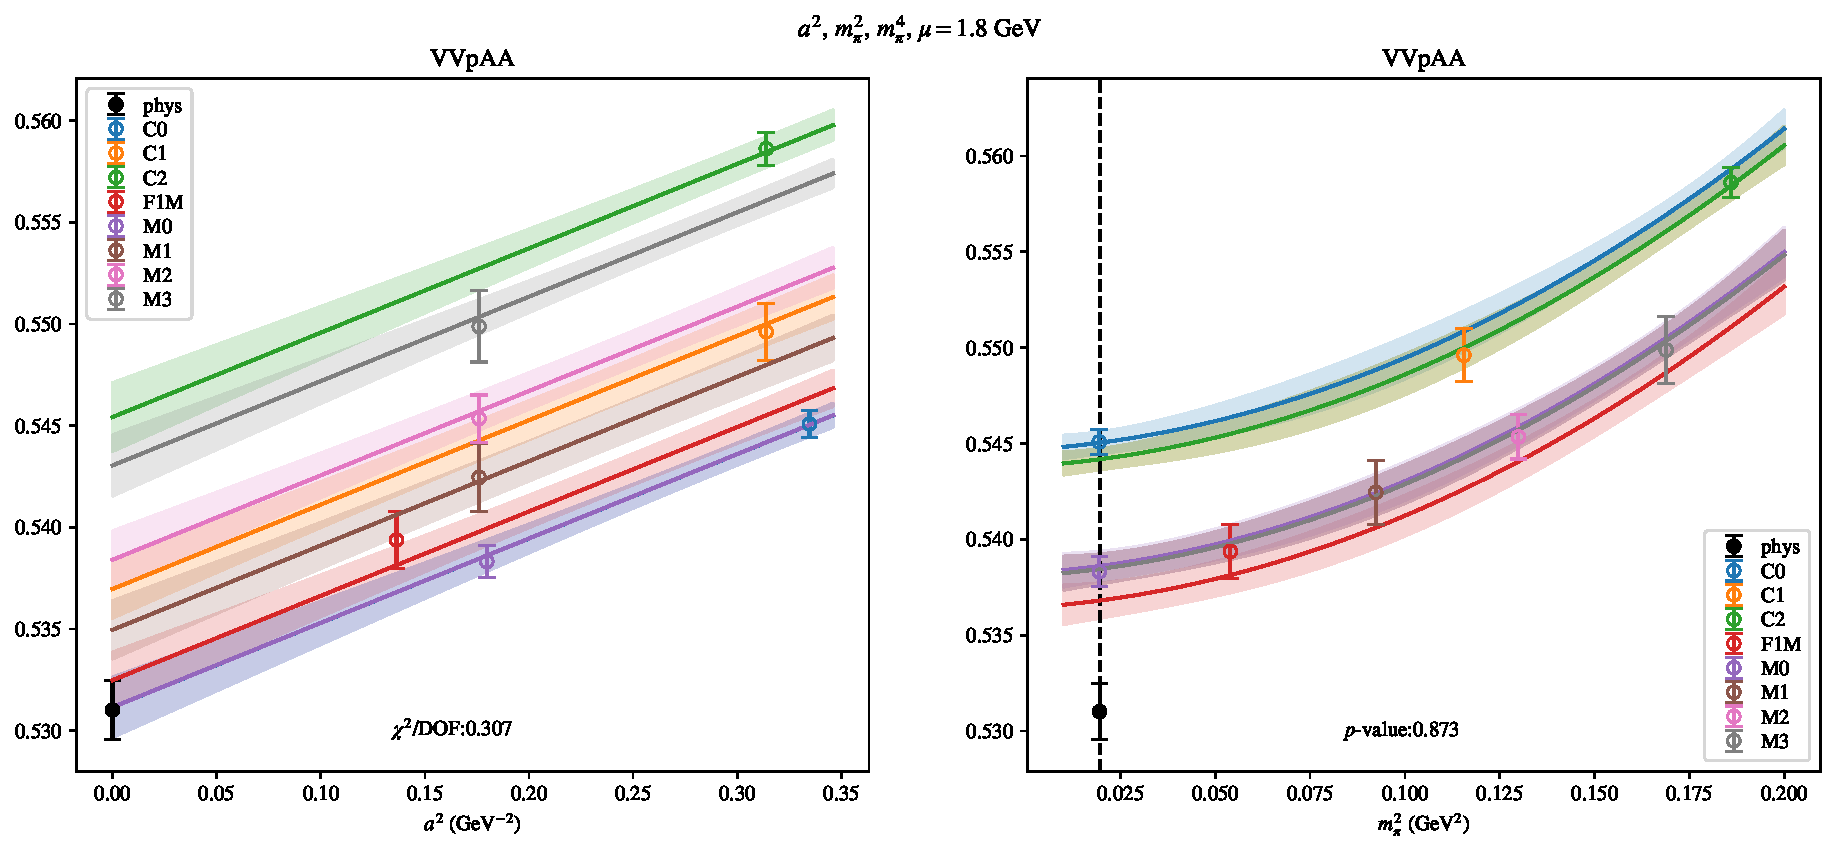
\includepdf[link, pages=-]{VVpAA/a2m2m4_18.pdf}
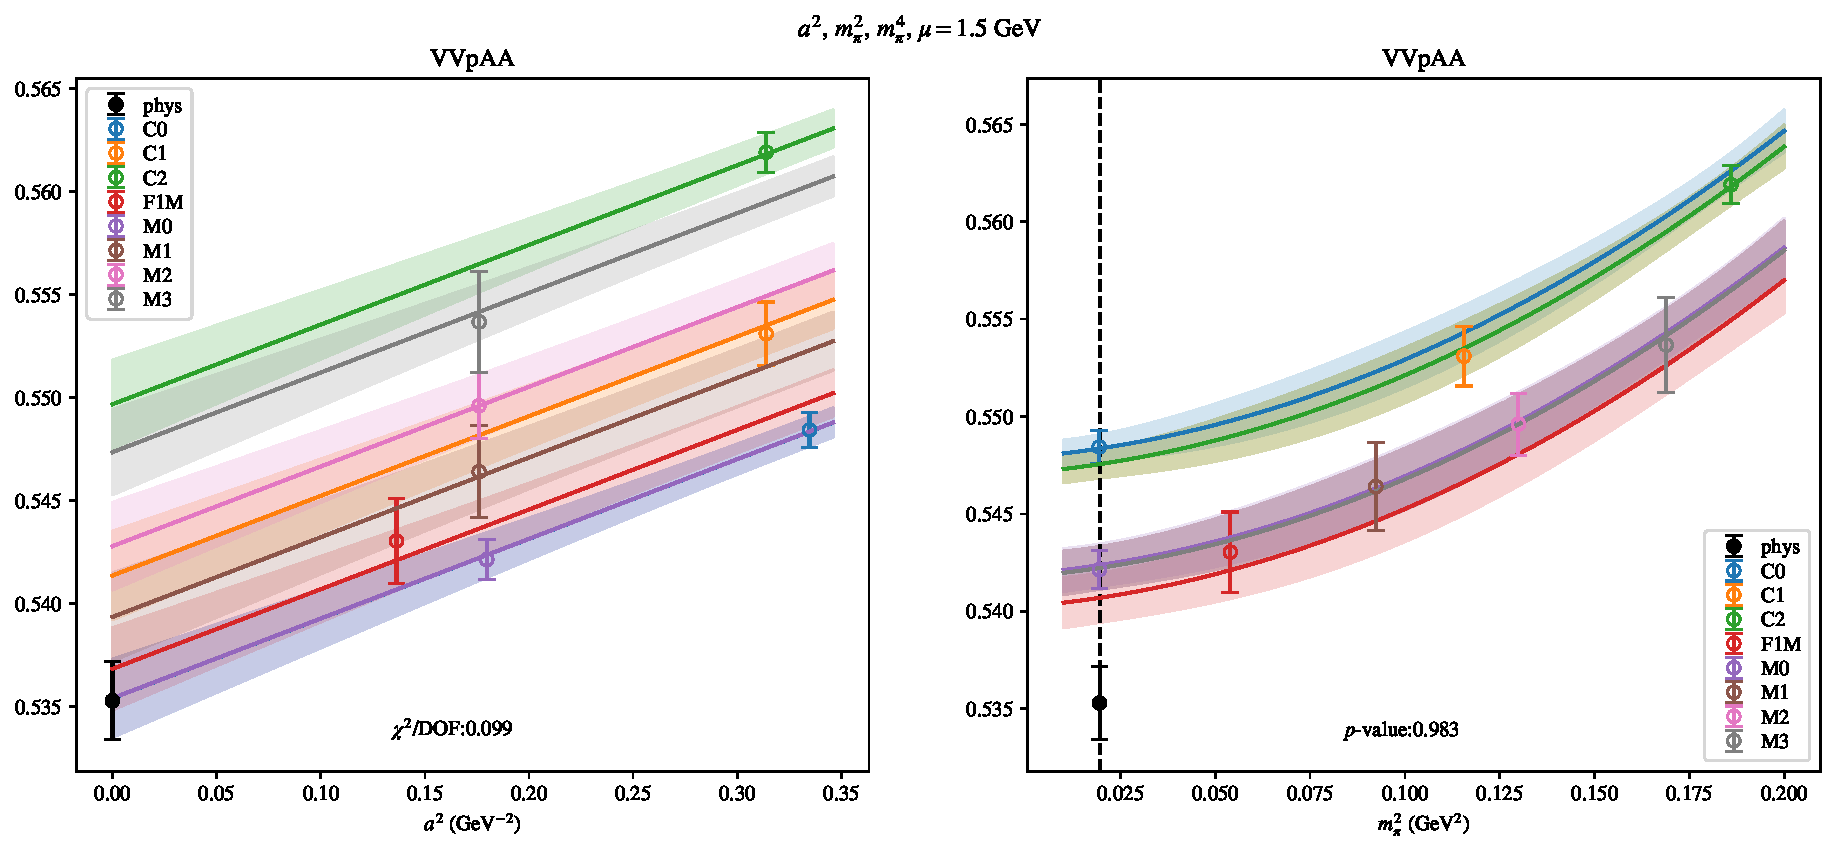
\includepdf[link, pages=-]{VVpAA/a2m2m4_15.pdf}
\clearpage
\section{VVmAA}
\begin{table}[!h]
\begin{center}
\begin{tabular*}{\linewidth}{@{\extracolsep{\fill}} |c|c|c|c|c|}
\hline
$\mu$ (GeV) & $a^2$, $m_\pi^2$ & $a^2$, $m_\pi^2$ no C & $a^2$, $a^4$, $m_\pi^2$ & $a^2$, $m_\pi^2$, $m_\pi^4$\\
\hline
2.0& \hyperlink{VVmAA/a2m2_20.pdf.1}{\textbf{2.3714(31)}: 8.812 (0.0)} & \hyperlink{VVmAA/a2m2noC_20.pdf.1}{\textbf{2.470(16)}: 0.354 (0.702)} & \hyperlink{VVmAA/a2a4m2_20.pdf.1}{\textbf{2.555(26)}: 0.418 (0.796)} & \hyperlink{VVmAA/a2m2m4_20.pdf.1}{\textbf{2.3688(31)}: 9.437 (0.0)}\\
1.8& \hyperlink{VVmAA/a2m2_18.pdf.1}{\textbf{2.5968(42)}: 8.923 (0.0)} & \hyperlink{VVmAA/a2m2noC_18.pdf.1}{\textbf{2.692(19)}: 0.993 (0.371)} & \hyperlink{VVmAA/a2a4m2_18.pdf.1}{\textbf{2.821(31)}: 2.489 (0.041)} & \hyperlink{VVmAA/a2m2m4_18.pdf.1}{\textbf{2.5945(40)}: 10.51 (0.0)}\\
1.5& \hyperlink{VVmAA/a2m2_15.pdf.1}{\textbf{2.9376(65)}: 9.386 (0.0)} & \hyperlink{VVmAA/a2m2noC_15.pdf.1}{\textbf{3.026(26)}: 1.469 (0.23)} & \hyperlink{VVmAA/a2a4m2_15.pdf.1}{\textbf{3.232(43)}: 5.497 (0.0)} & \hyperlink{VVmAA/a2m2m4_15.pdf.1}{\textbf{2.9360(58)}: 11.616 (0.0)}\\
\hline
\end{tabular*}
\caption{Physical point value from chiral and continuum extrapolation at renormalisation scale $\mu$. Entries are \textbf{value(error)}: $\chi^2/\text{DOF}$ ($p$-value).}
\end{center}
\end{table}
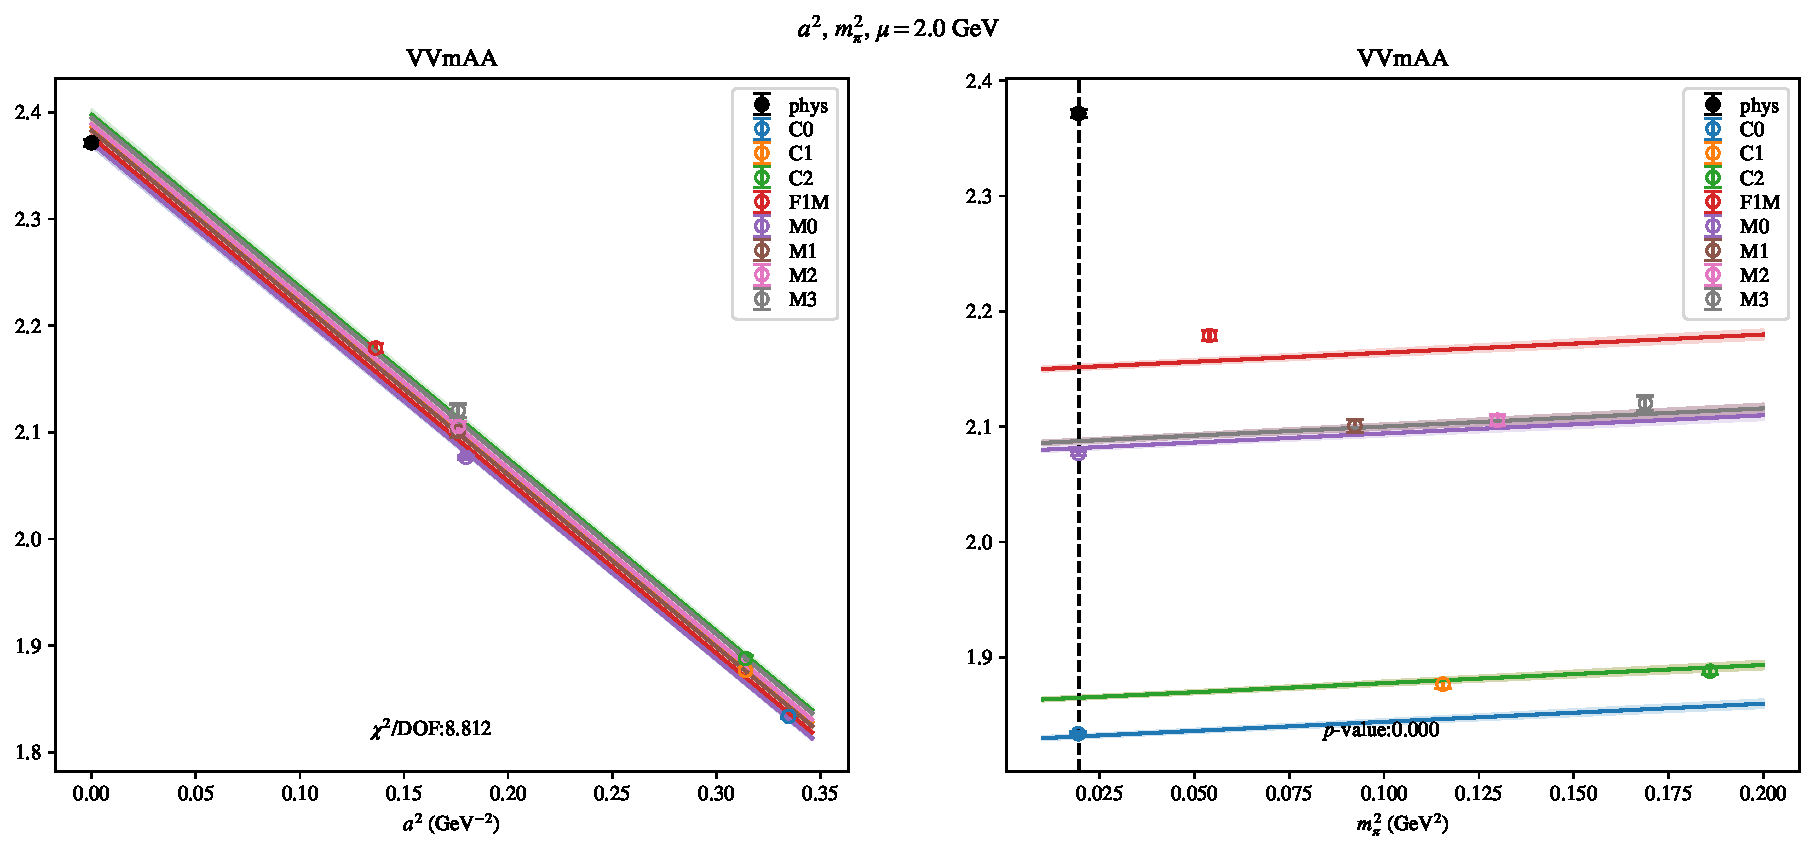
\includepdf[link, pages=-]{VVmAA/a2m2_20.pdf}
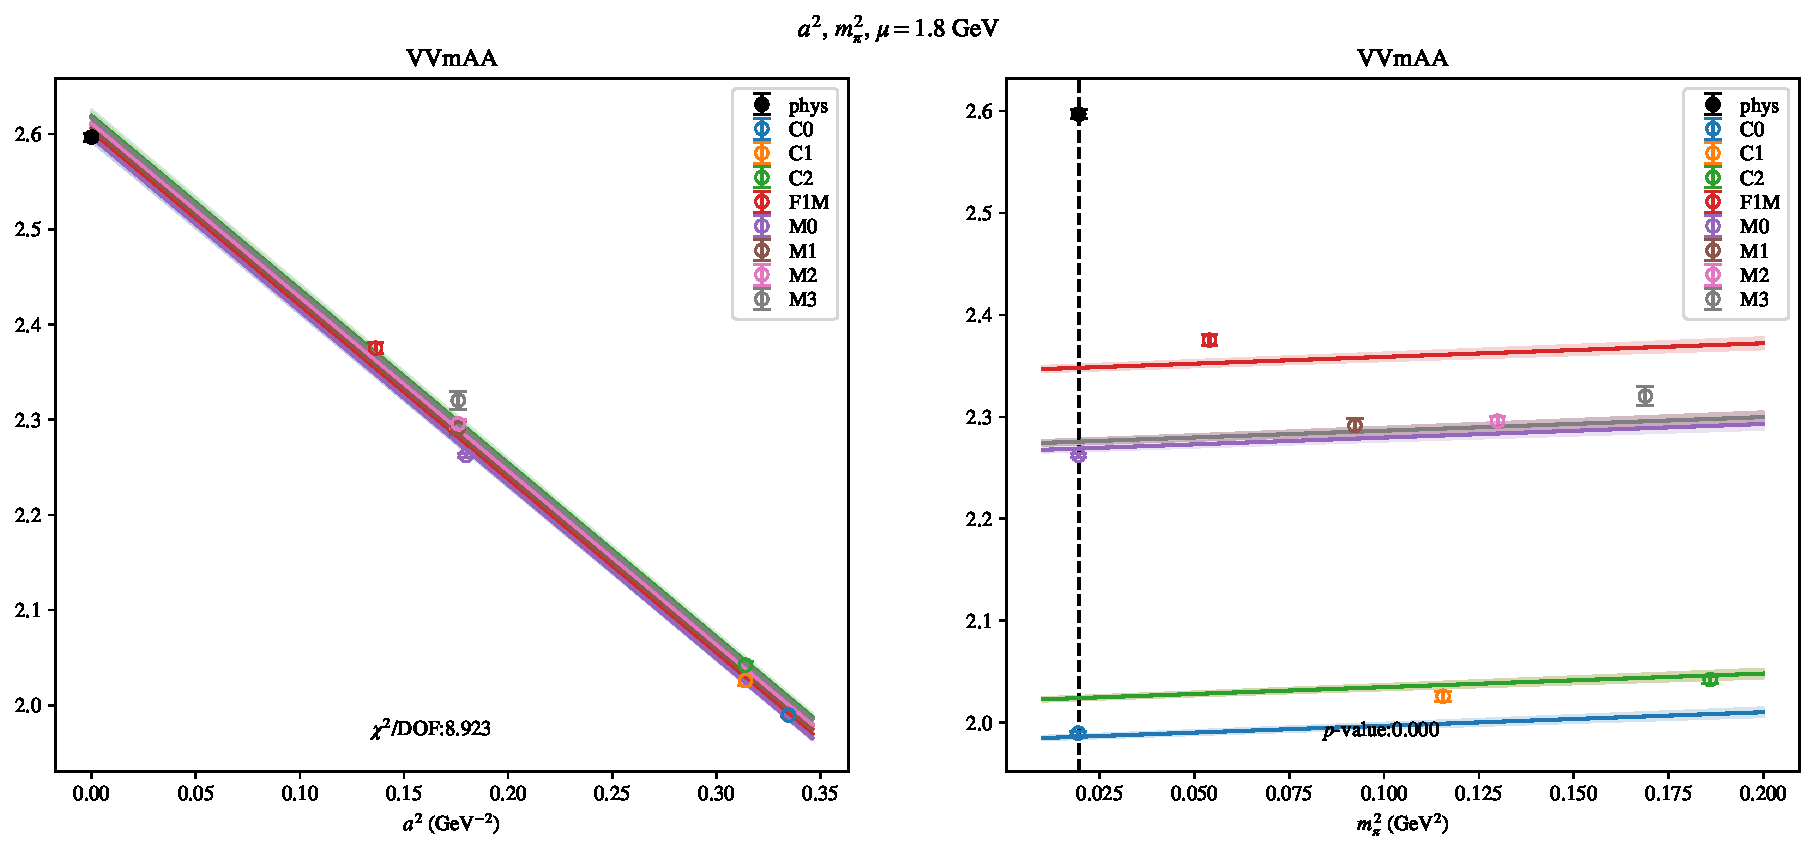
\includepdf[link, pages=-]{VVmAA/a2m2_18.pdf}
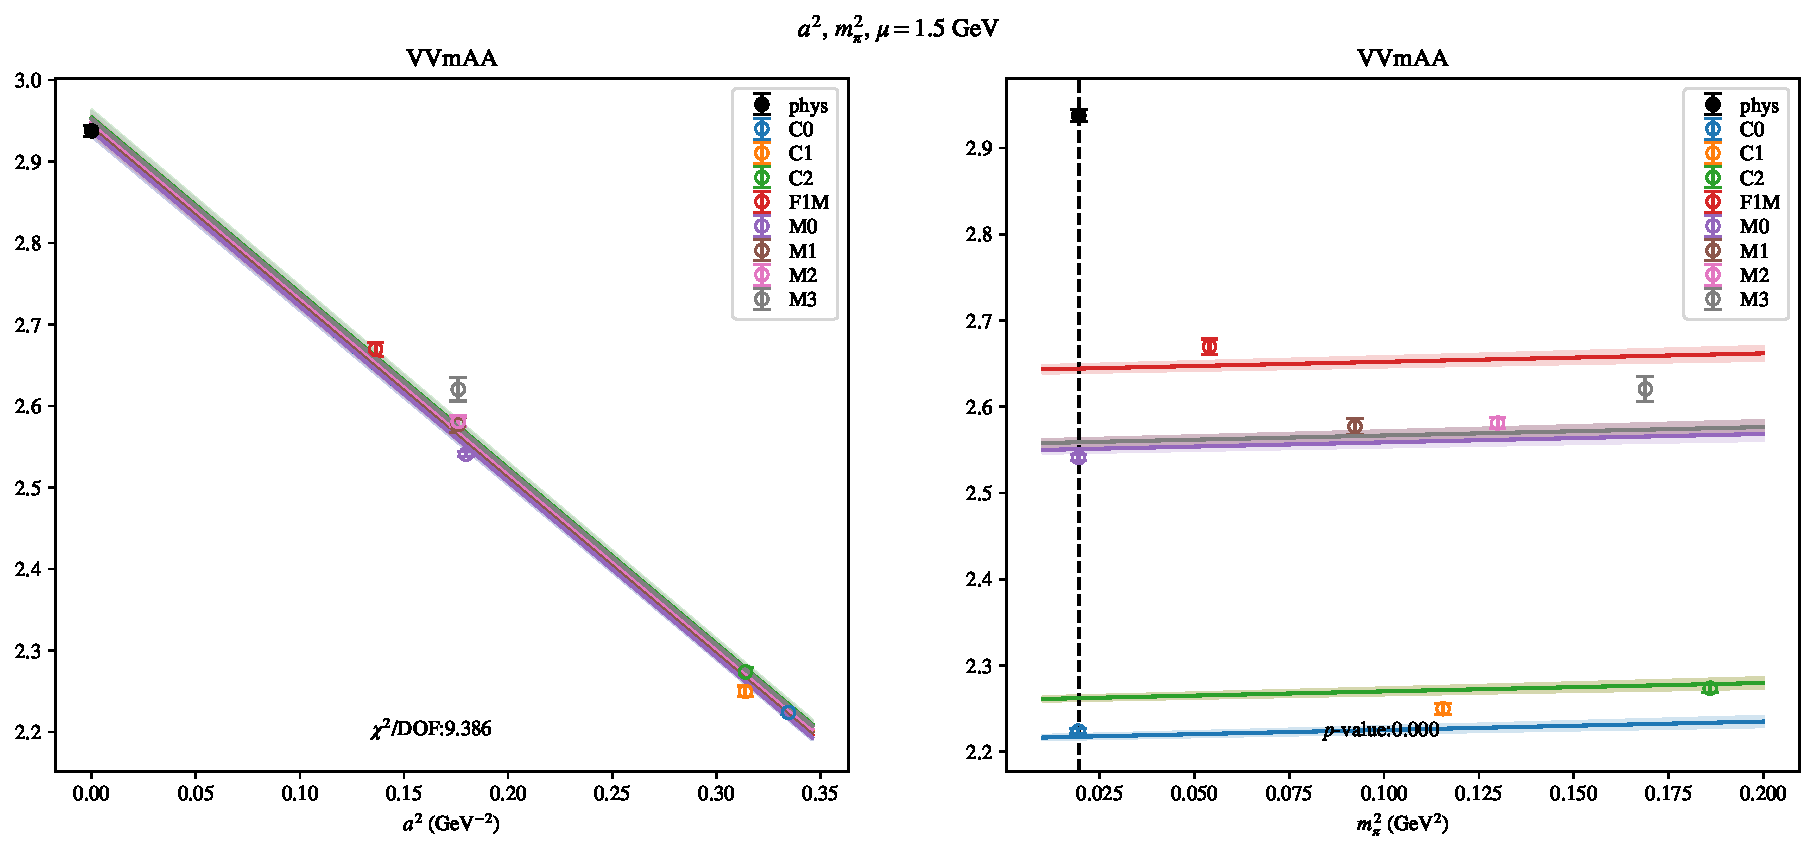
\includepdf[link, pages=-]{VVmAA/a2m2_15.pdf}
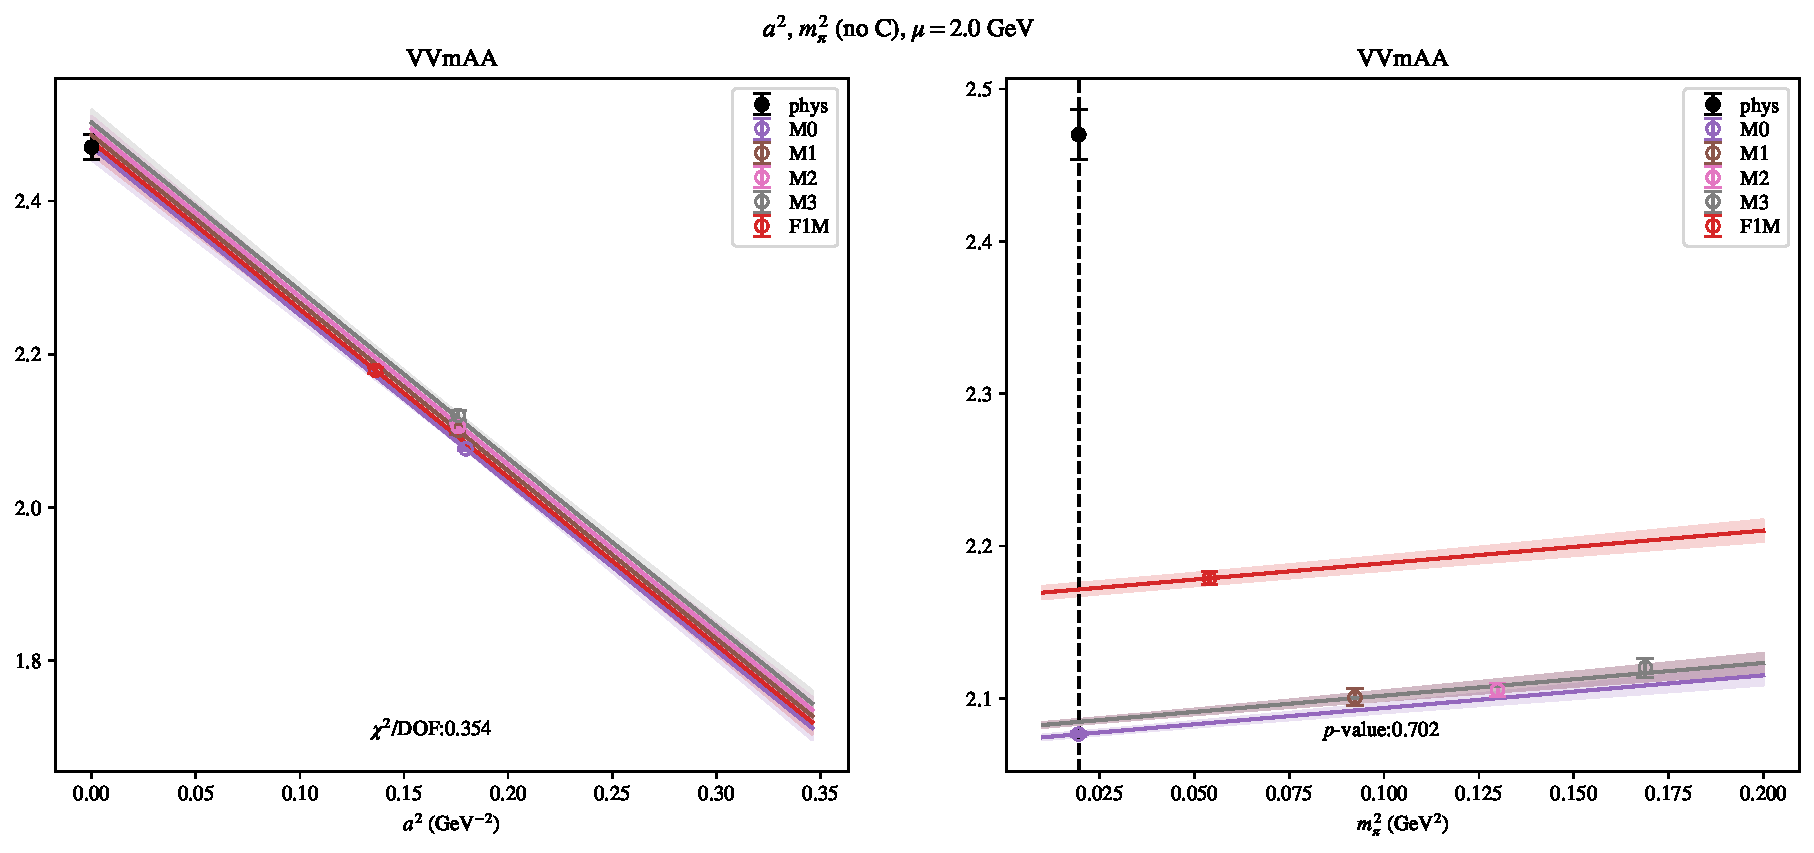
\includepdf[link, pages=-]{VVmAA/a2m2noC_20.pdf}
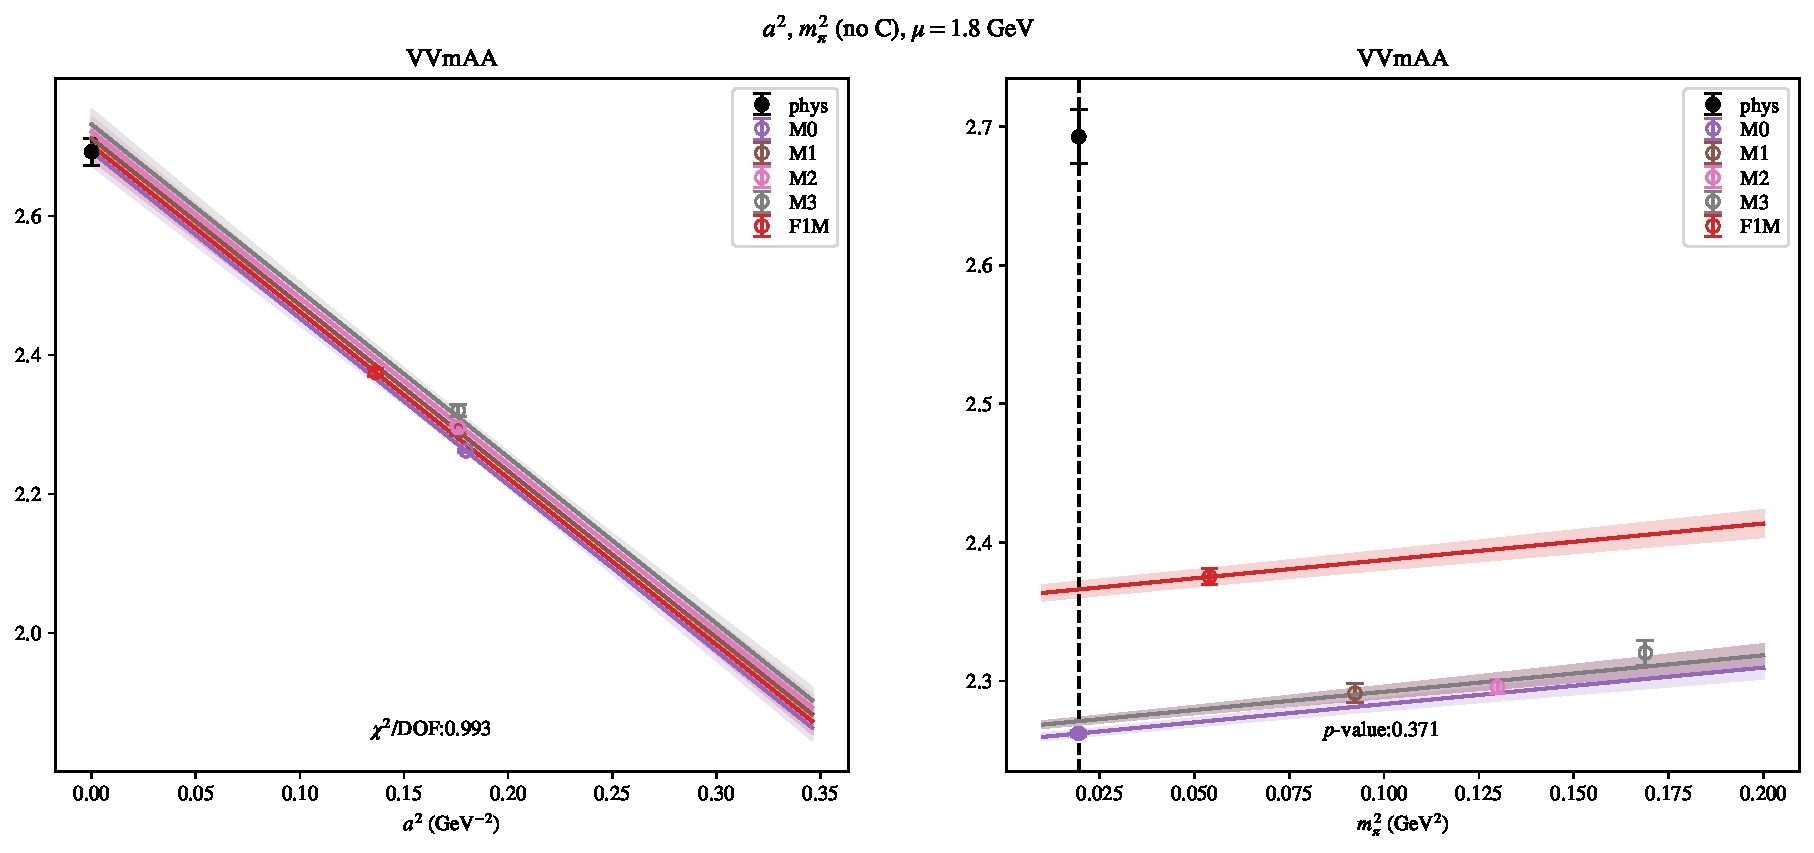
\includepdf[link, pages=-]{VVmAA/a2m2noC_18.pdf}
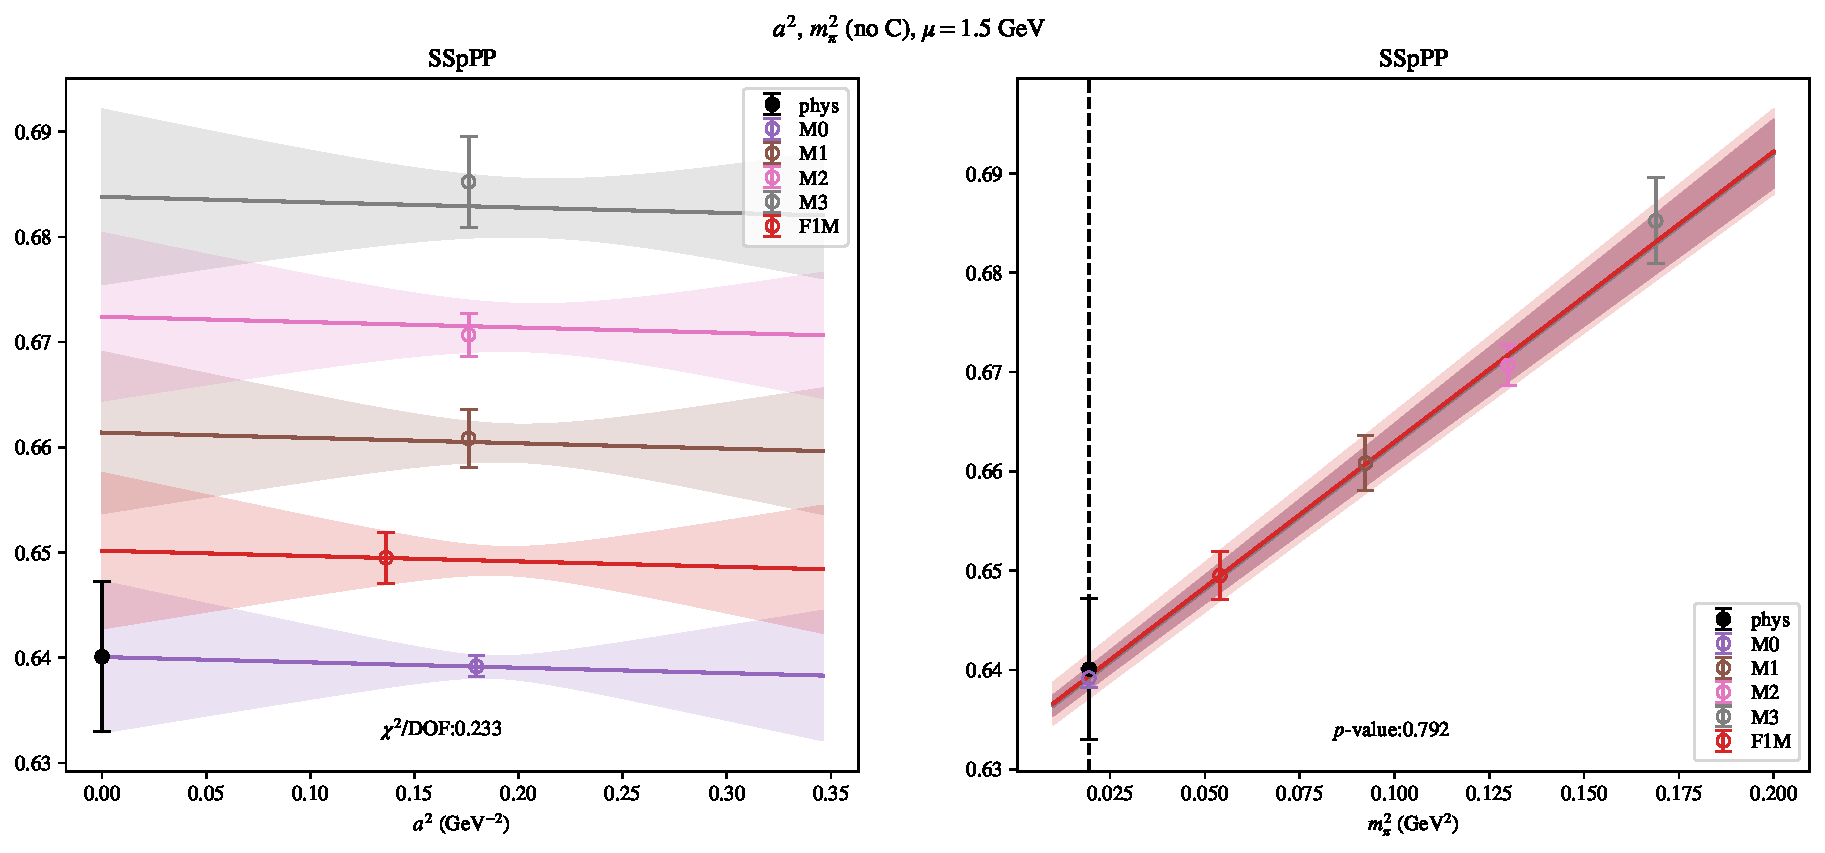
\includepdf[link, pages=-]{VVmAA/a2m2noC_15.pdf}
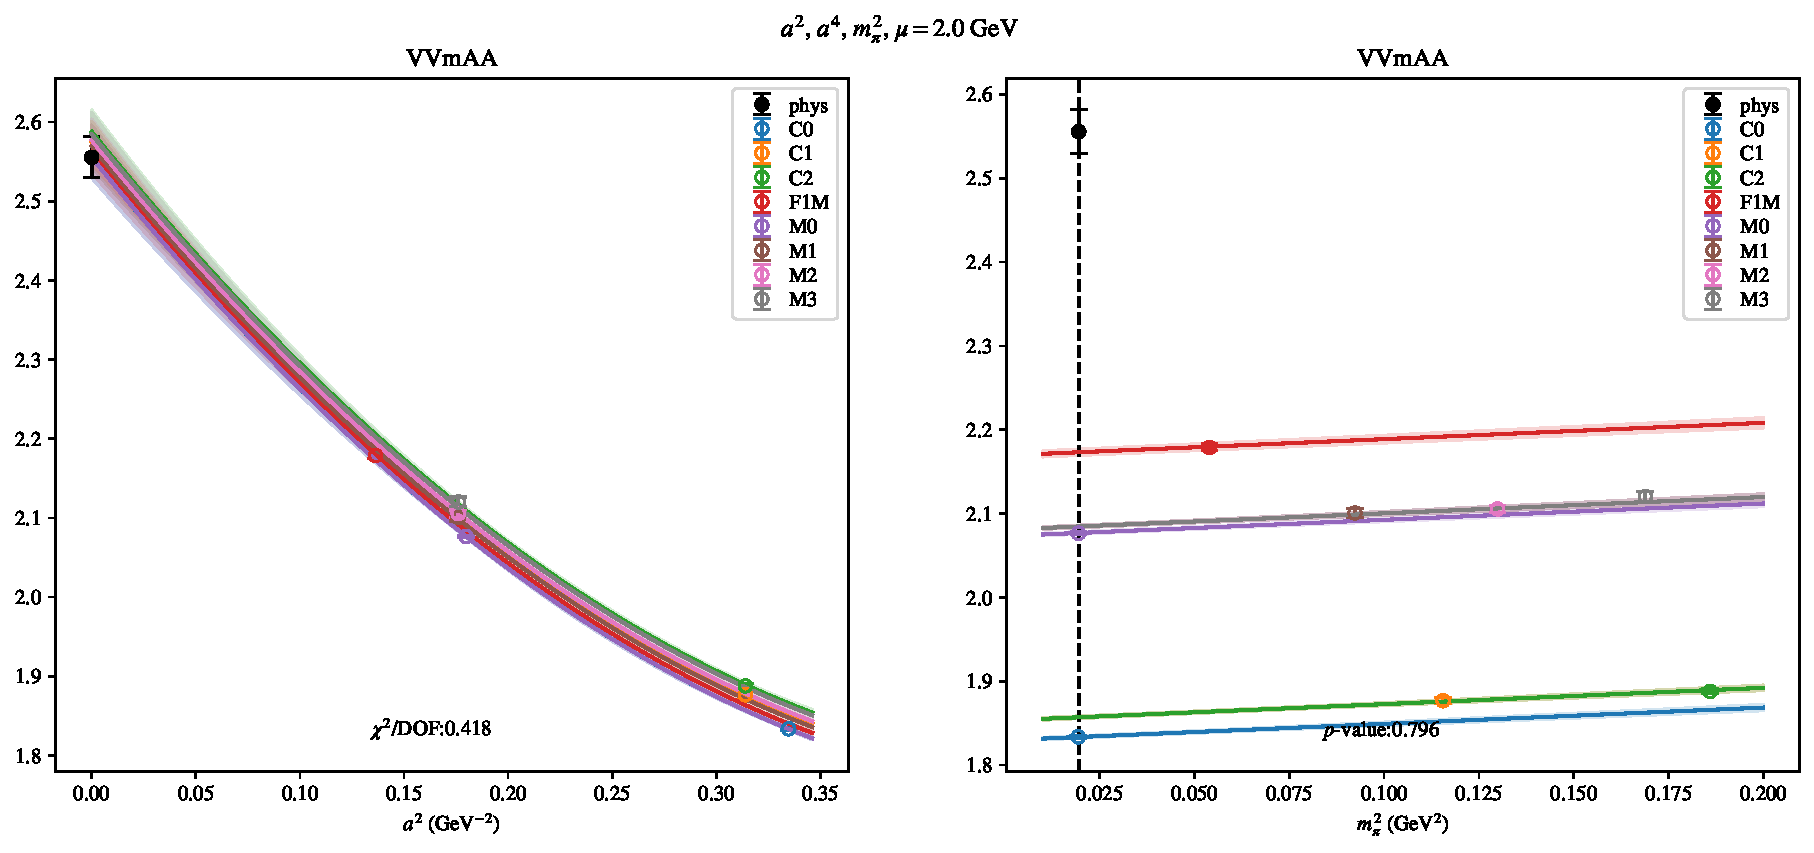
\includepdf[link, pages=-]{VVmAA/a2a4m2_20.pdf}
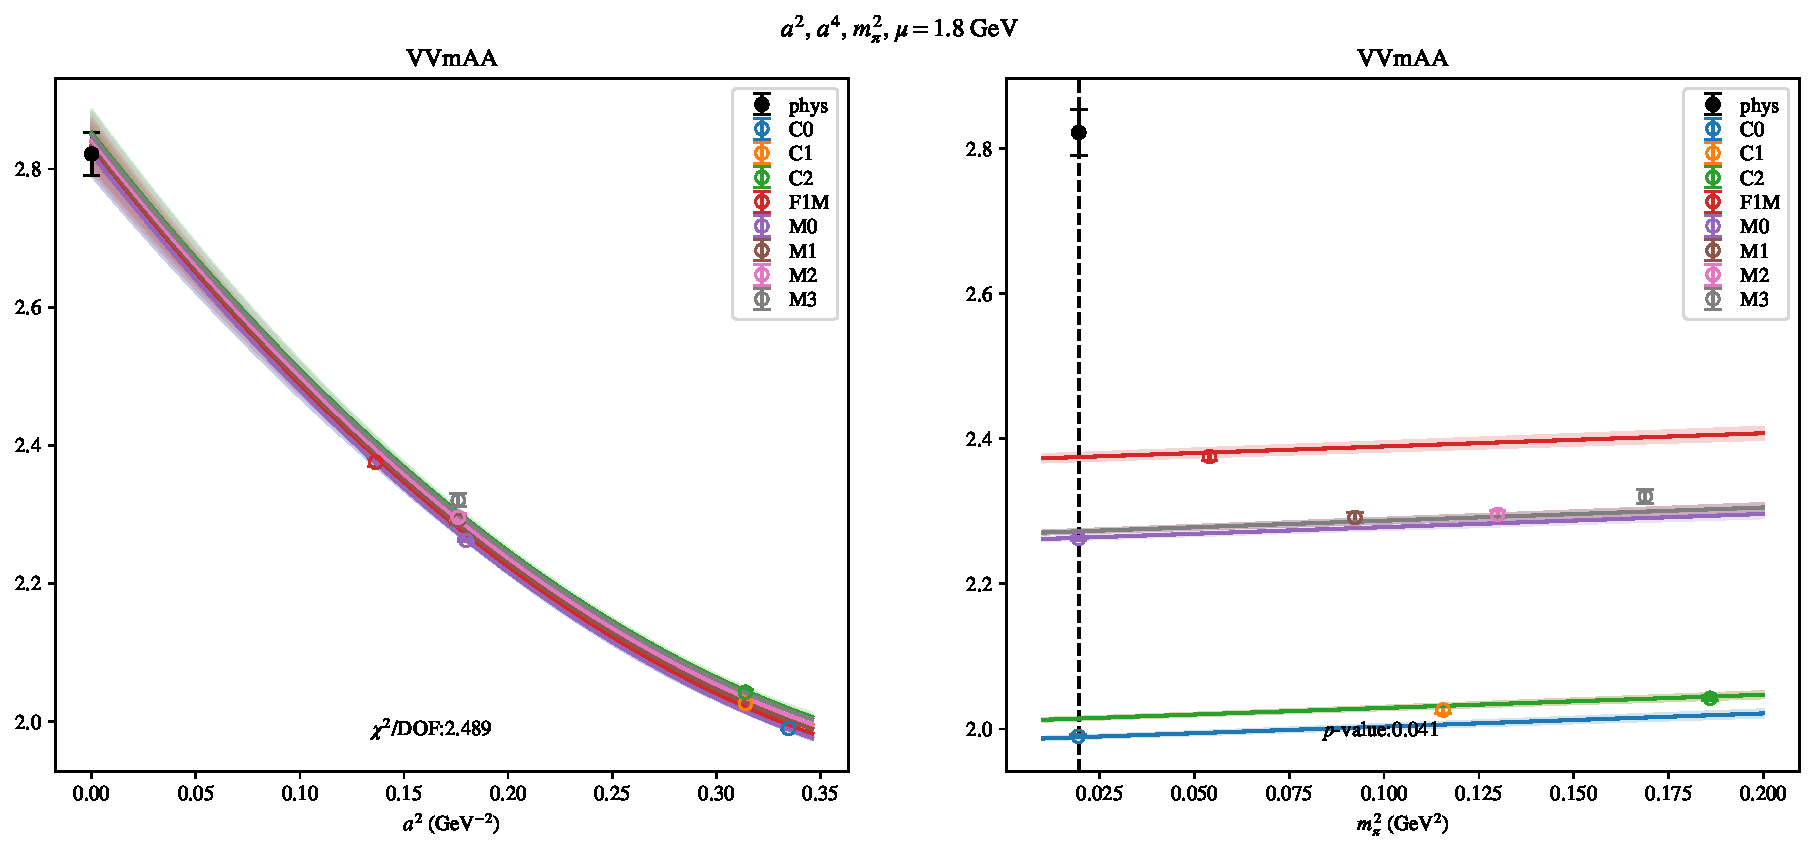
\includepdf[link, pages=-]{VVmAA/a2a4m2_18.pdf}
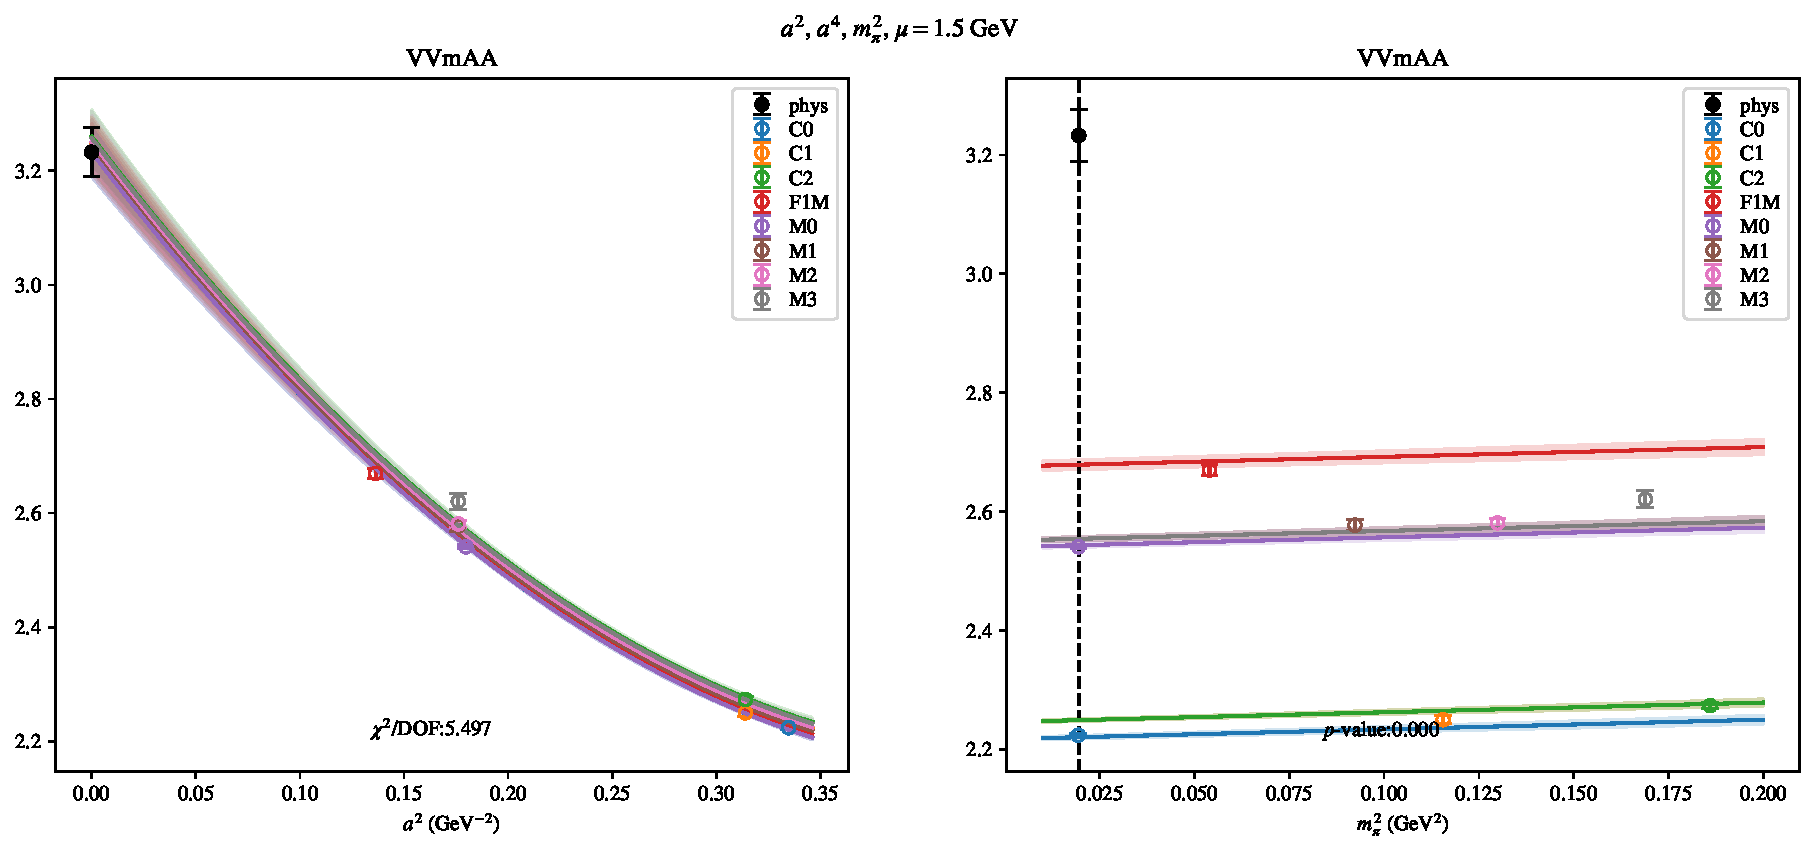
\includepdf[link, pages=-]{VVmAA/a2a4m2_15.pdf}
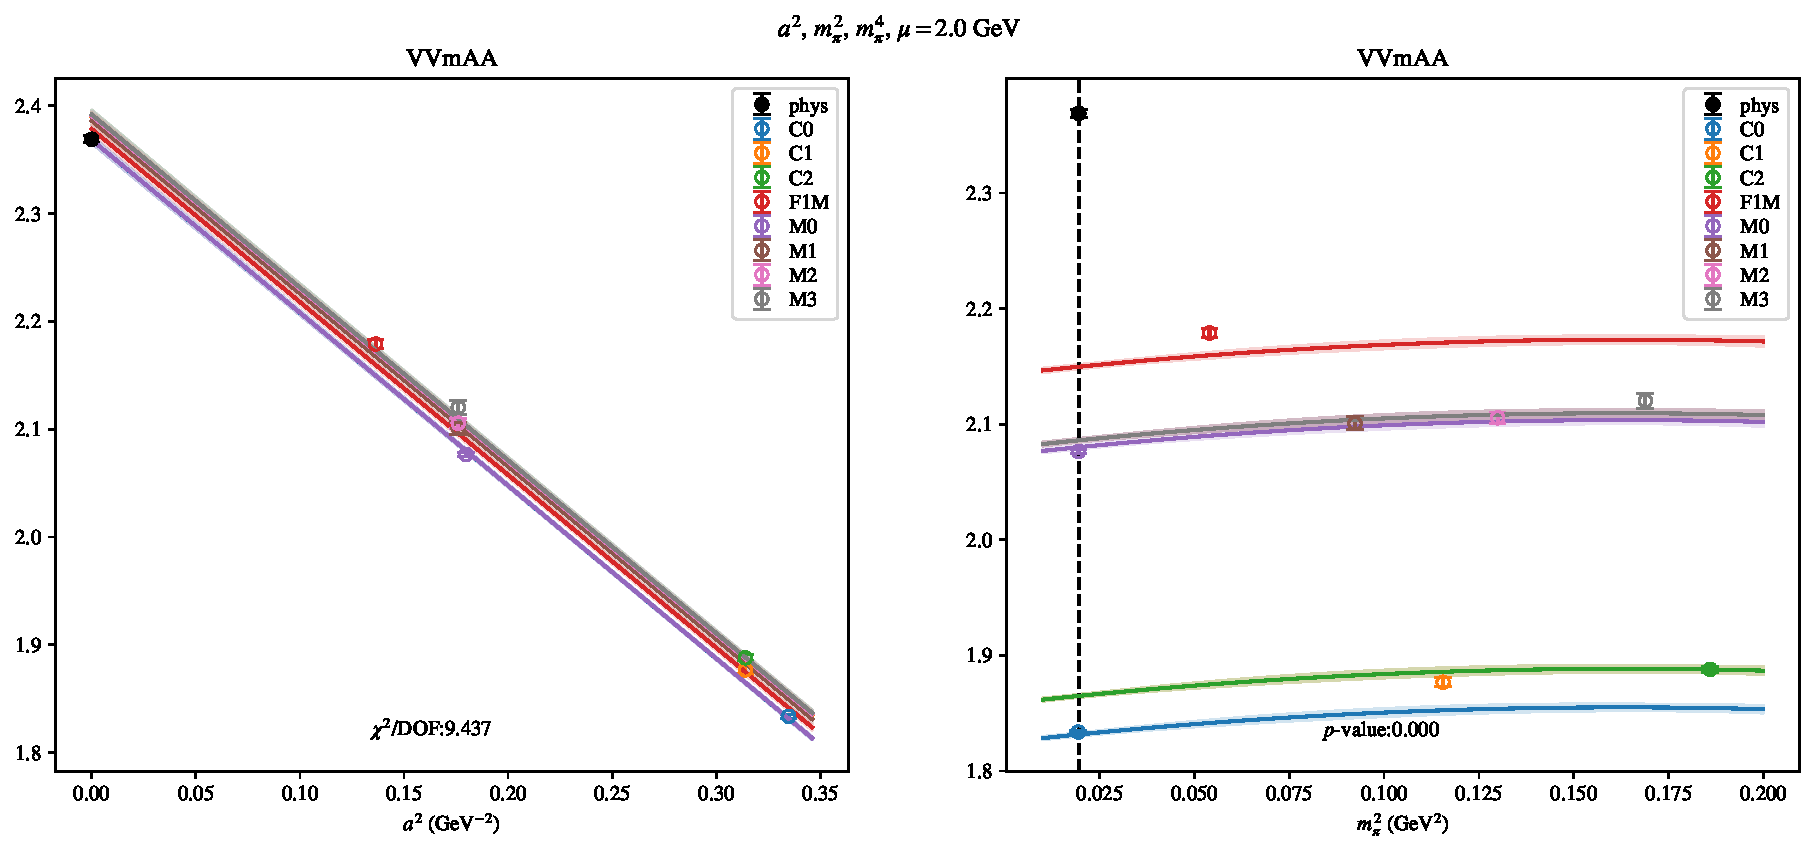
\includepdf[link, pages=-]{VVmAA/a2m2m4_20.pdf}
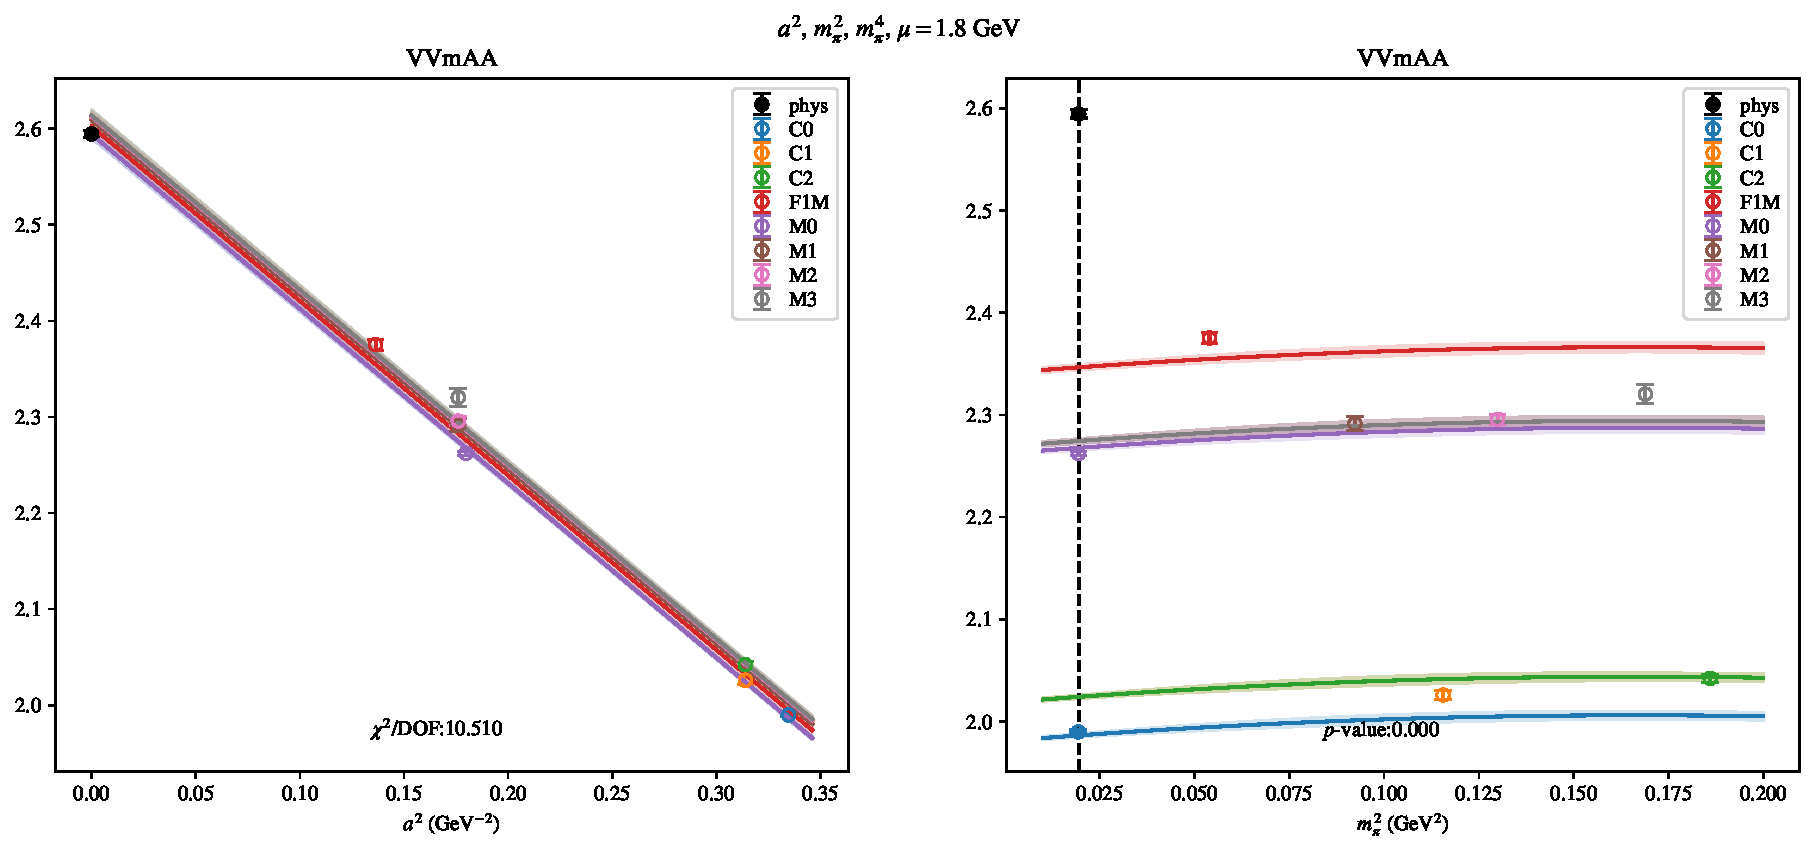
\includepdf[link, pages=-]{VVmAA/a2m2m4_18.pdf}
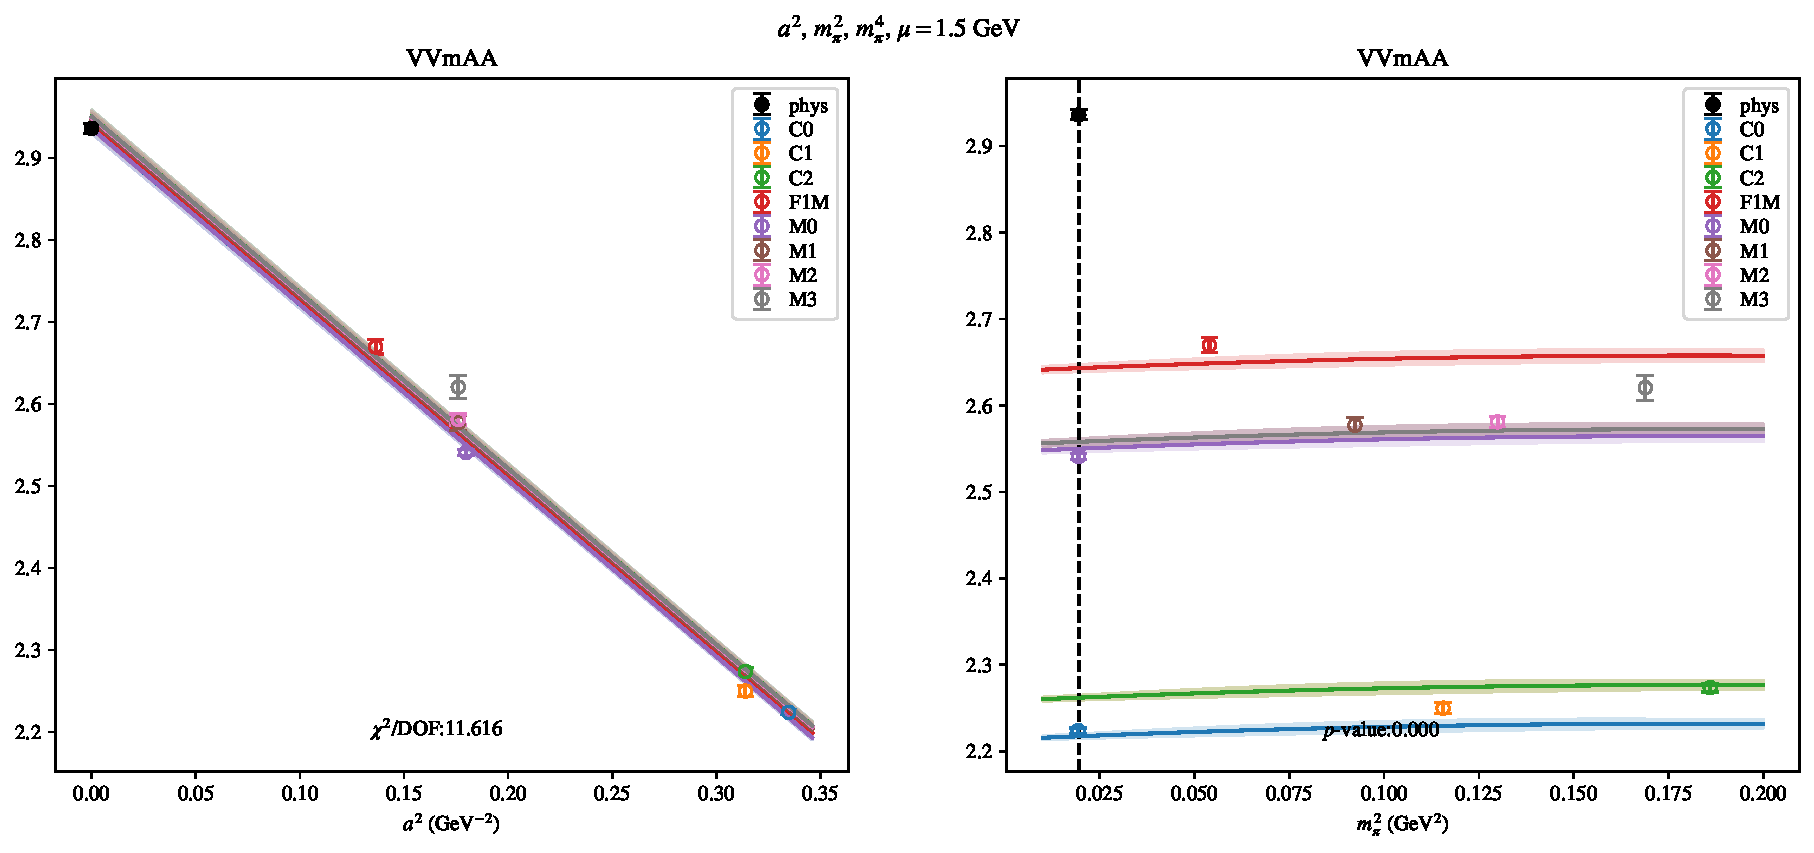
\includepdf[link, pages=-]{VVmAA/a2m2m4_15.pdf}
\clearpage
\section{SSmPP}
\begin{table}[!h]
\begin{center}
\begin{tabular*}{\linewidth}{@{\extracolsep{\fill}} |c|c|c|c|c|}
\hline
$\mu$ (GeV) & $a^2$, $m_\pi^2$ & $a^2$, $m_\pi^2$ no C & $a^2$, $a^4$, $m_\pi^2$ & $a^2$, $m_\pi^2$, $m_\pi^4$\\
\hline
2.0& \hyperlink{SSmPP/a2m2_20.pdf.1}{\textbf{0.9557(14)}: 4.069 (0.001)} & \hyperlink{SSmPP/a2m2noC_20.pdf.1}{\textbf{0.9259(67)}: 1.711 (0.181)} & \hyperlink{SSmPP/a2a4m2_20.pdf.1}{\textbf{0.906(11)}: 1.012 (0.4)} & \hyperlink{SSmPP/a2m2m4_20.pdf.1}{\textbf{0.9572(15)}: 3.563 (0.007)}\\
1.8& \hyperlink{SSmPP/a2m2_18.pdf.1}{\textbf{0.9631(18)}: 2.42 (0.033)} & \hyperlink{SSmPP/a2m2noC_18.pdf.1}{\textbf{0.9365(74)}: 2.117 (0.12)} & \hyperlink{SSmPP/a2a4m2_18.pdf.1}{\textbf{0.922(12)}: 1.336 (0.254)} & \hyperlink{SSmPP/a2m2m4_18.pdf.1}{\textbf{0.9647(17)}: 1.96 (0.098)}\\
1.5& \hyperlink{SSmPP/a2m2_15.pdf.1}{\textbf{0.9741(27)}: 1.372 (0.231)} & \hyperlink{SSmPP/a2m2noC_15.pdf.1}{\textbf{0.9523(94)}: 2.007 (0.134)} & \hyperlink{SSmPP/a2a4m2_15.pdf.1}{\textbf{0.947(15)}: 1.41 (0.228)} & \hyperlink{SSmPP/a2m2m4_15.pdf.1}{\textbf{0.9759(24)}: 1.054 (0.378)}\\
\hline
\end{tabular*}
\caption{Physical point value from chiral and continuum extrapolation at renormalisation scale $\mu$. Entries are \textbf{value(error)}: $\chi^2/\text{DOF}$ ($p$-value).}
\end{center}
\end{table}
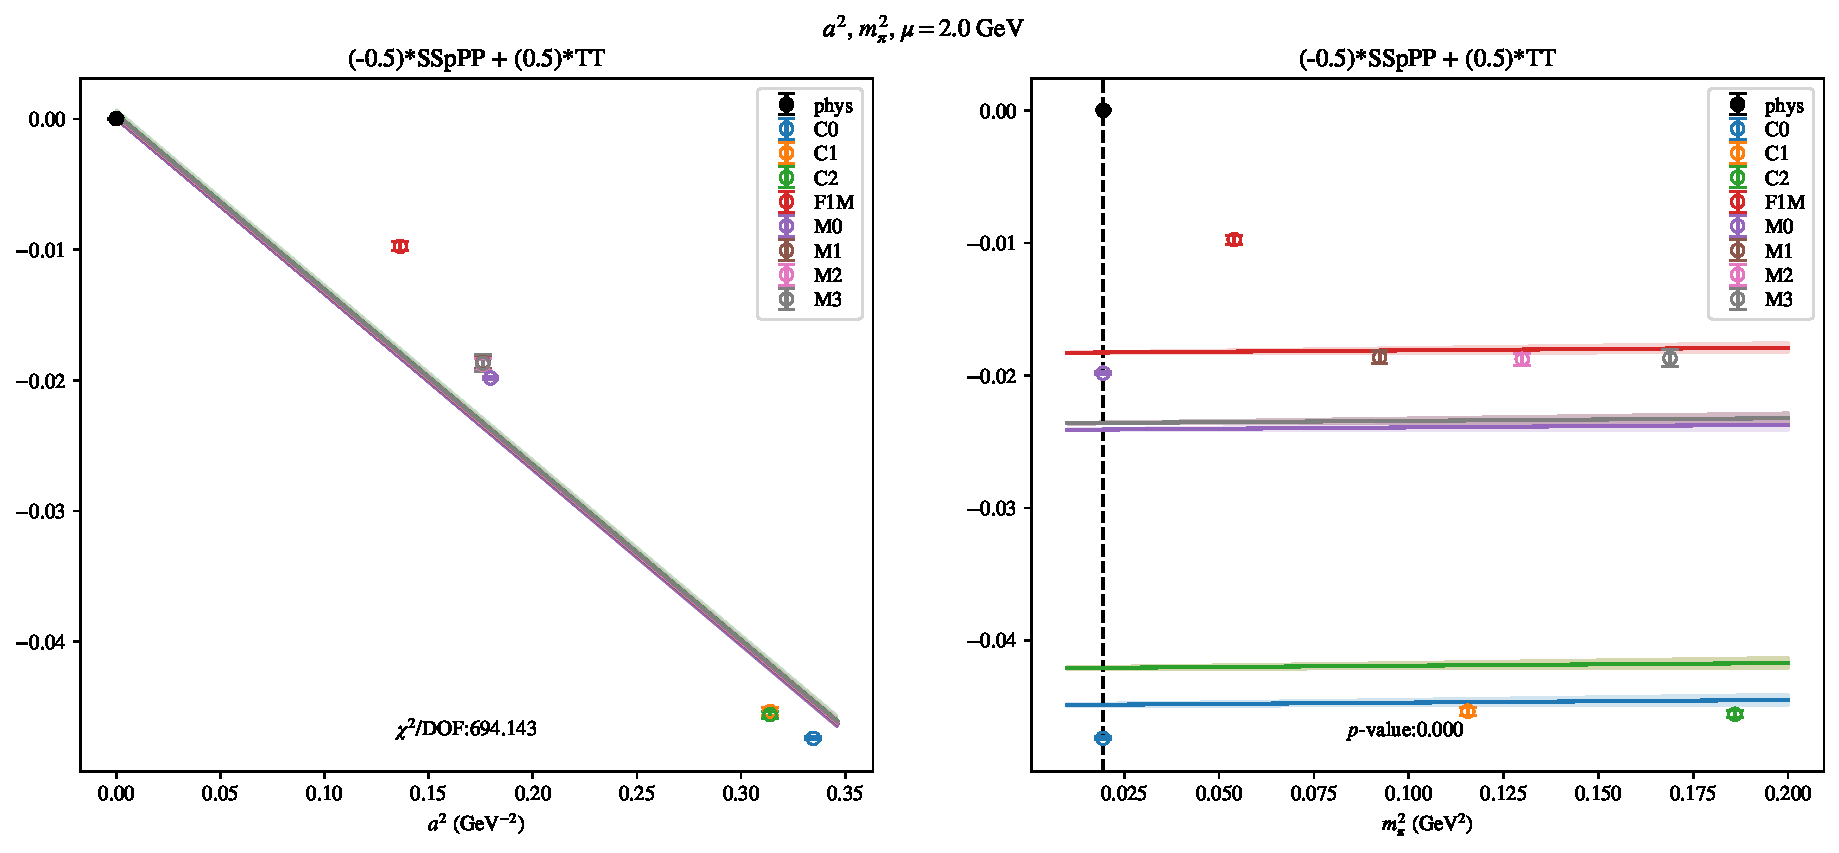
\includepdf[link, pages=-]{SSmPP/a2m2_20.pdf}
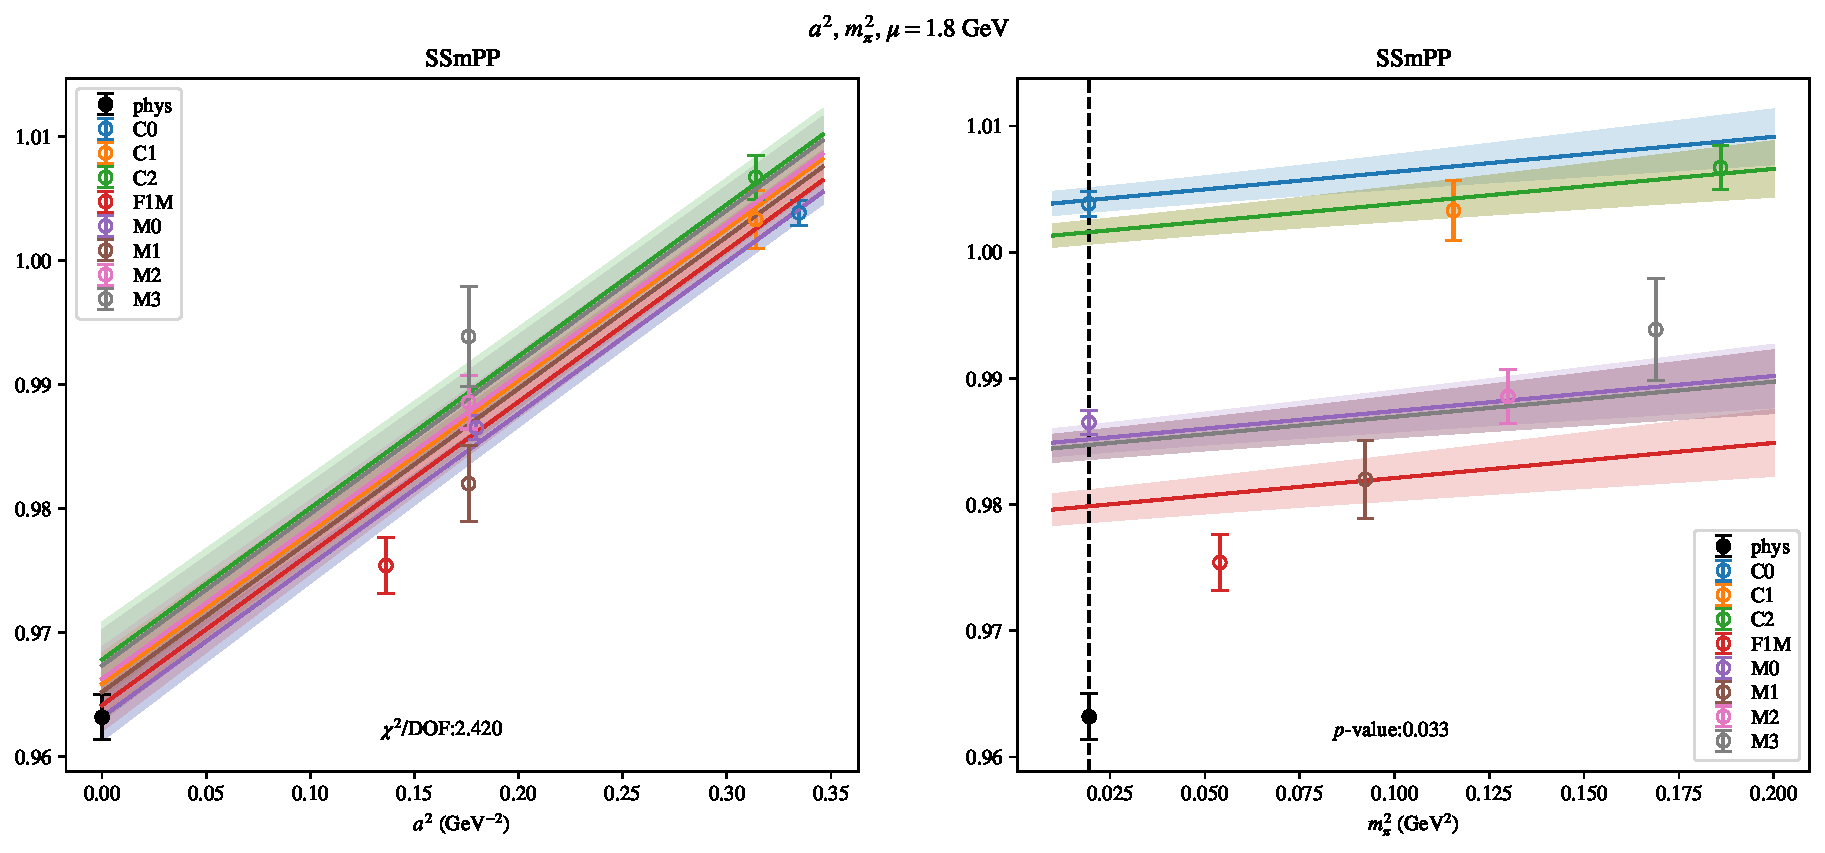
\includepdf[link, pages=-]{SSmPP/a2m2_18.pdf}
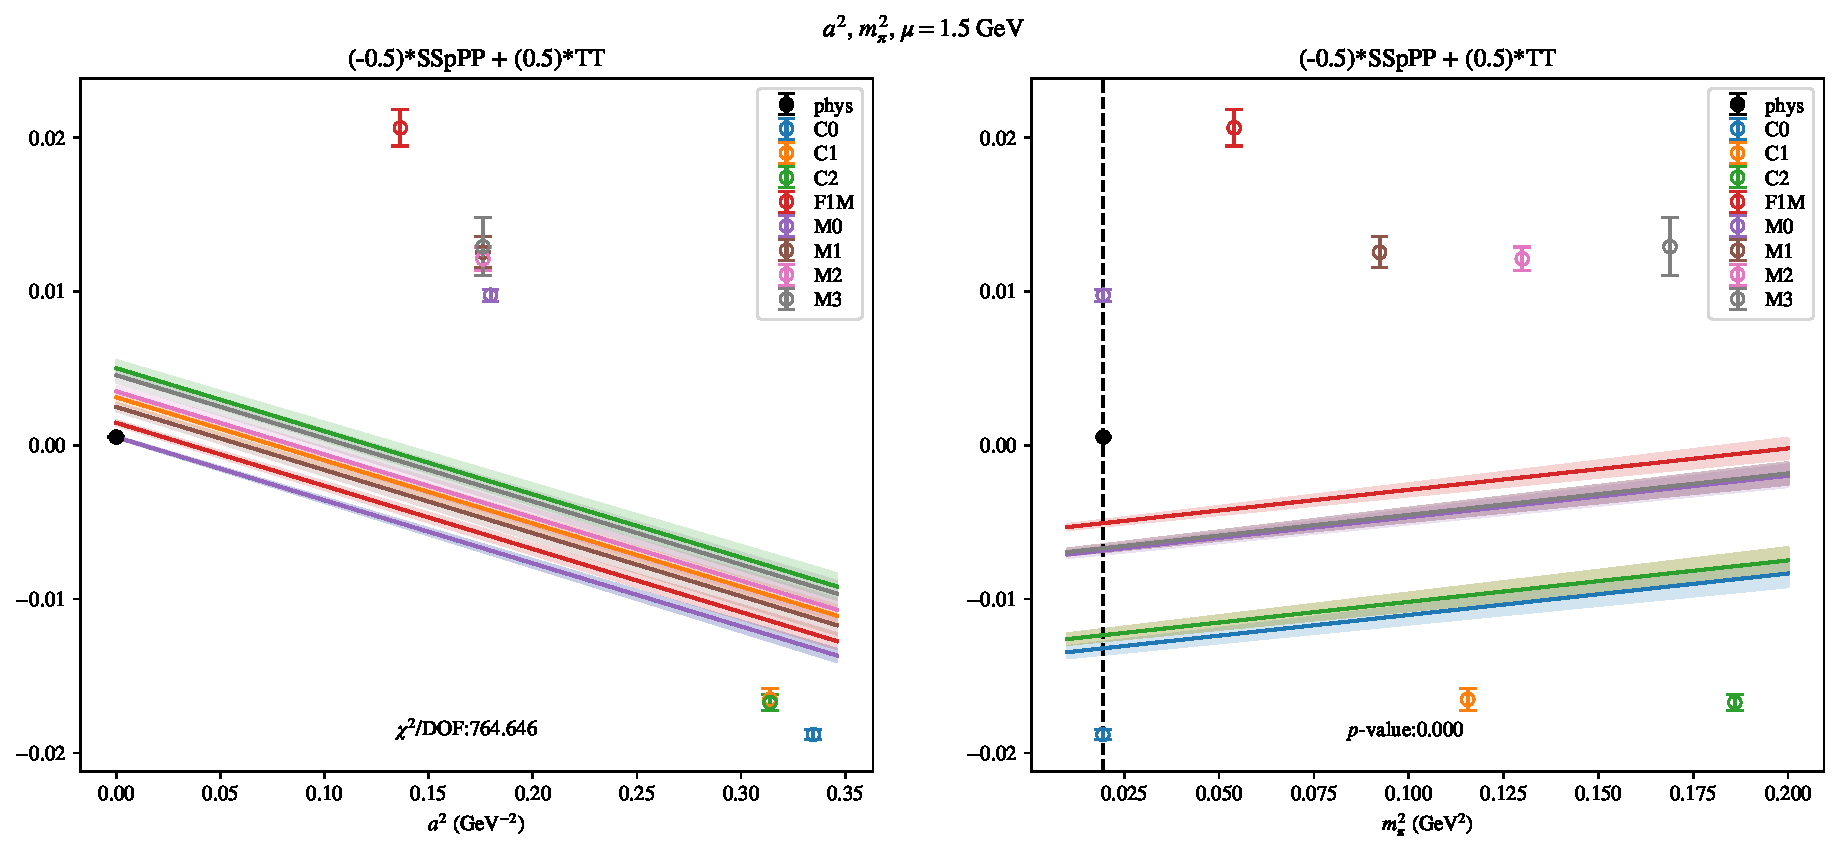
\includepdf[link, pages=-]{SSmPP/a2m2_15.pdf}
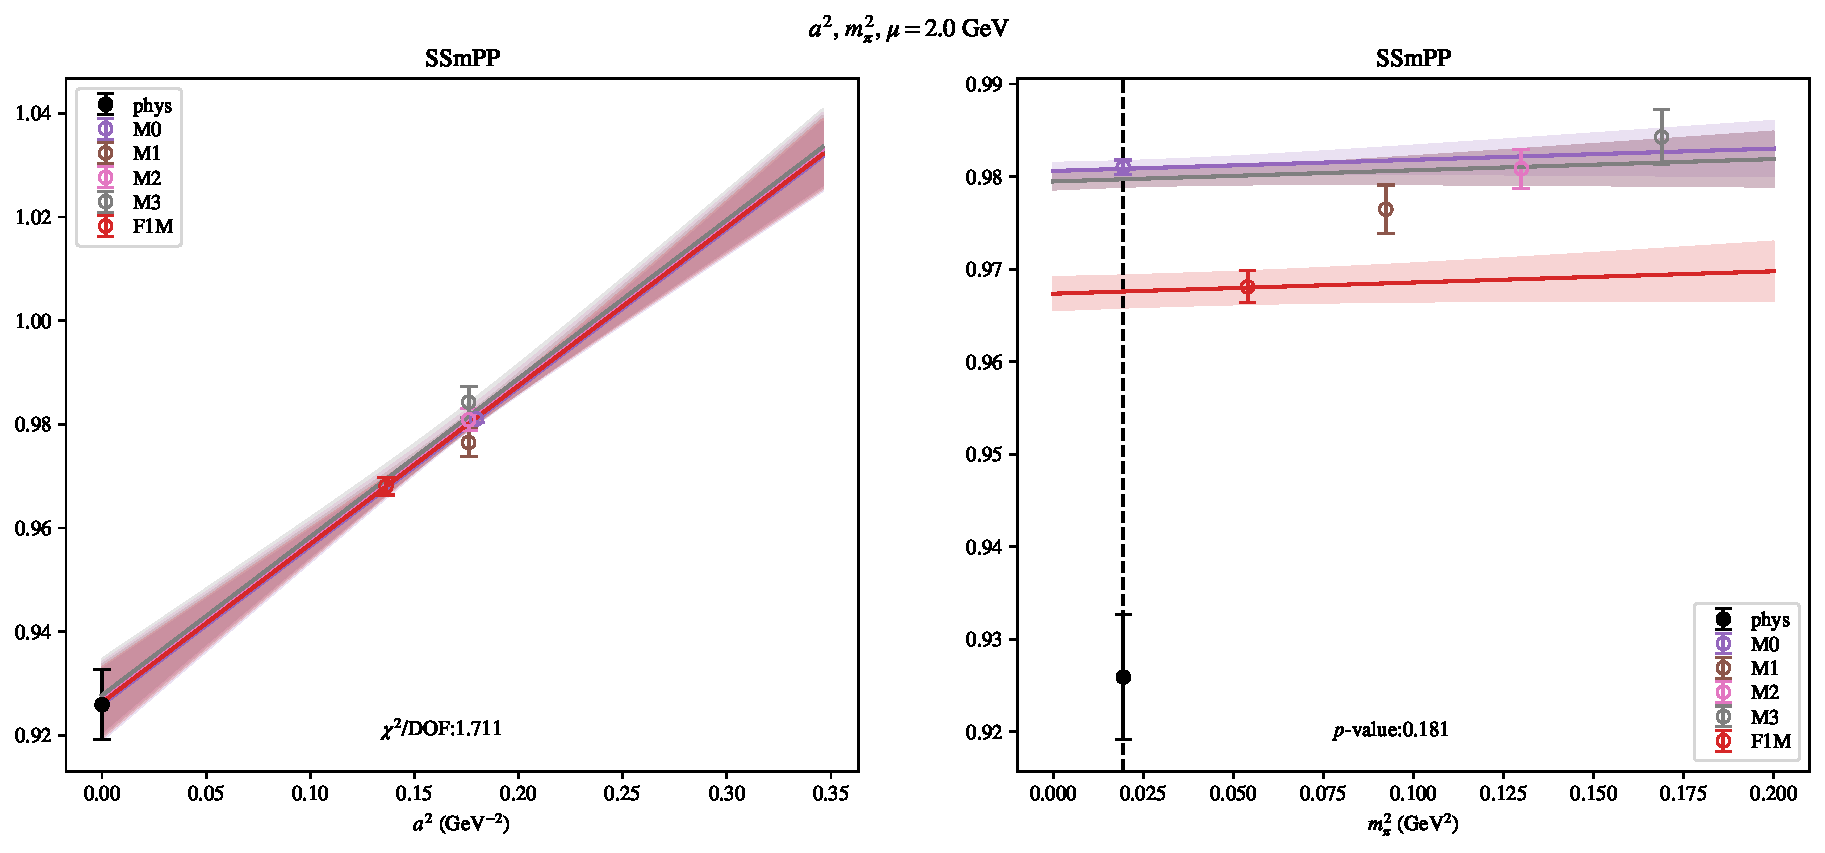
\includepdf[link, pages=-]{SSmPP/a2m2noC_20.pdf}
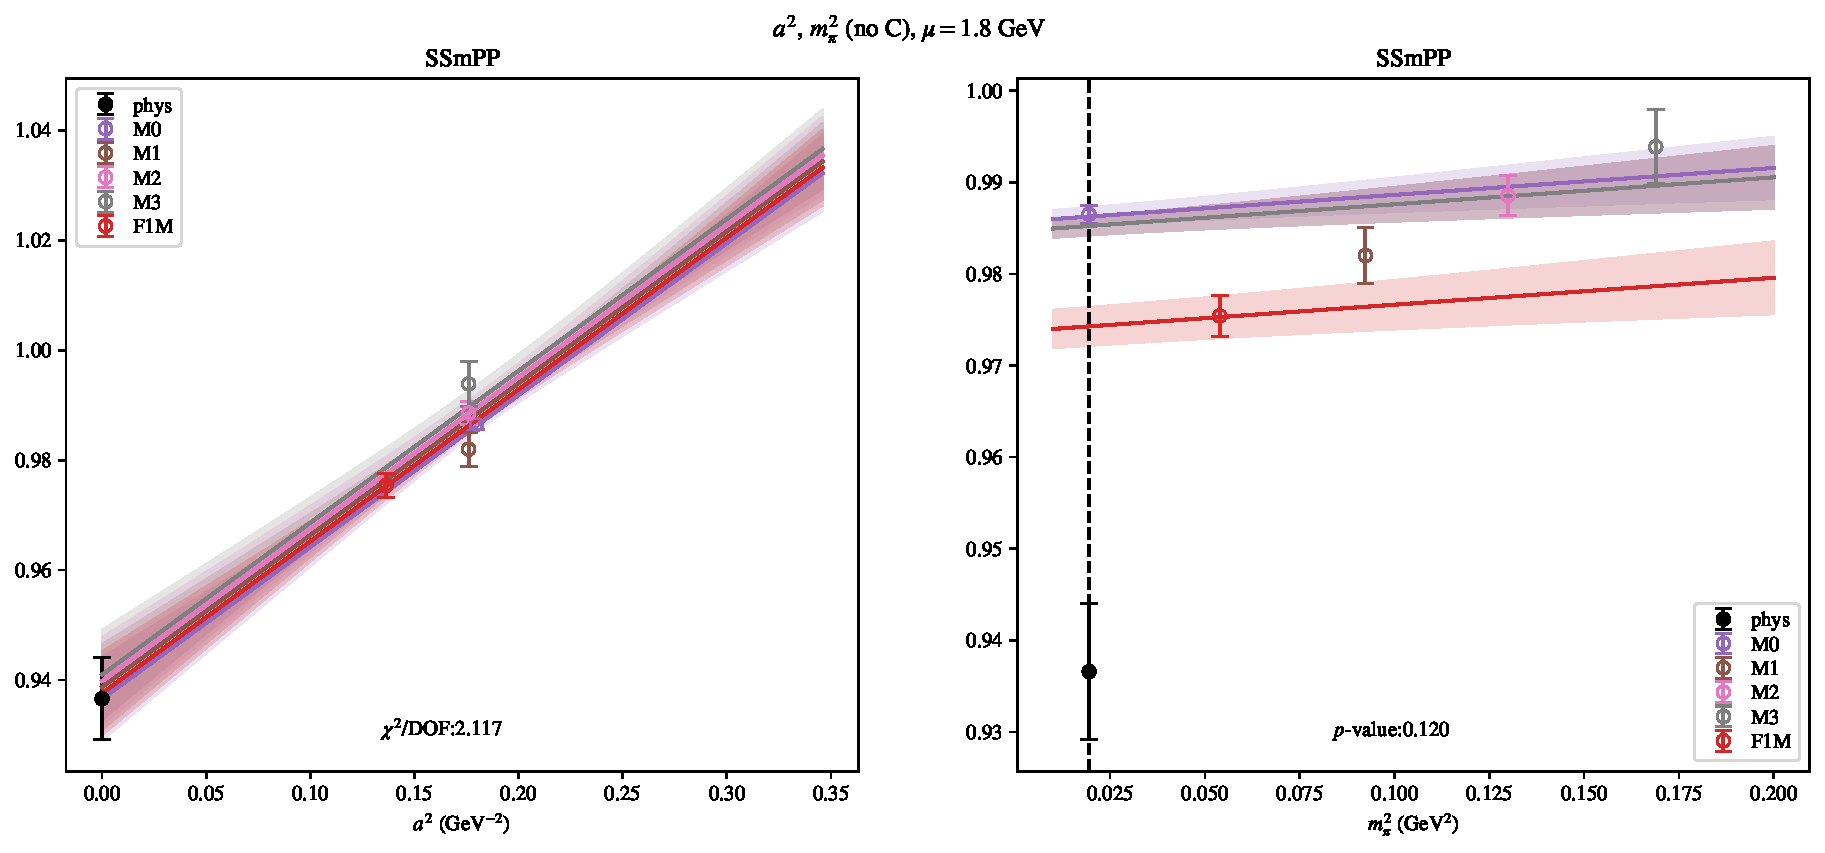
\includepdf[link, pages=-]{SSmPP/a2m2noC_18.pdf}
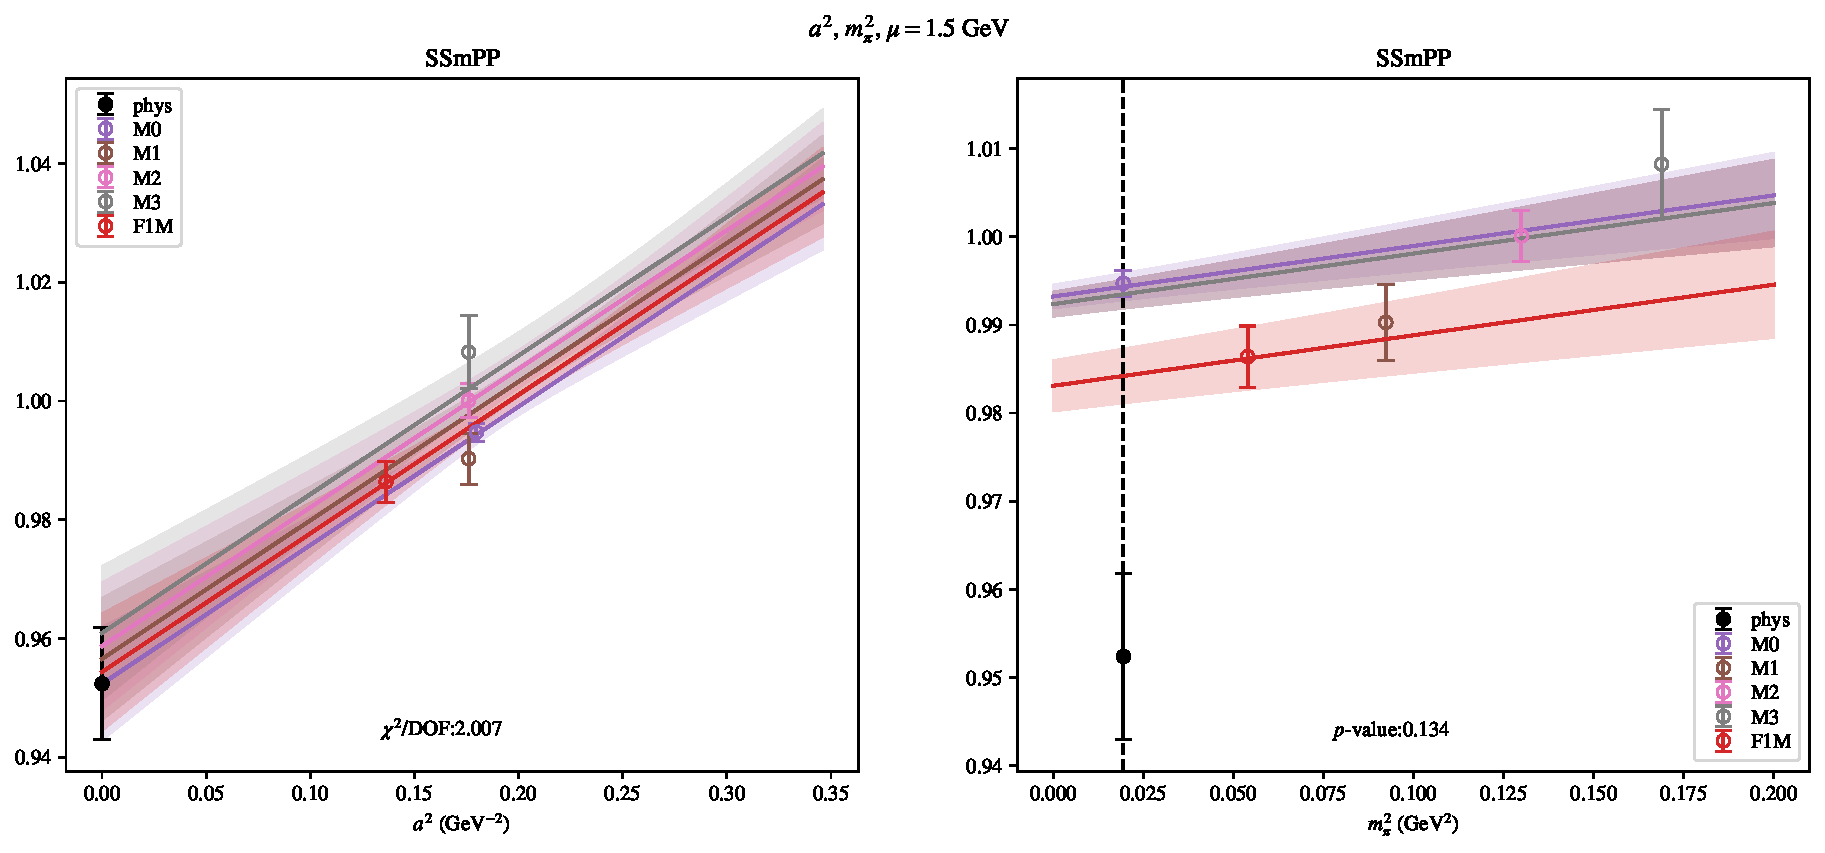
\includepdf[link, pages=-]{SSmPP/a2m2noC_15.pdf}
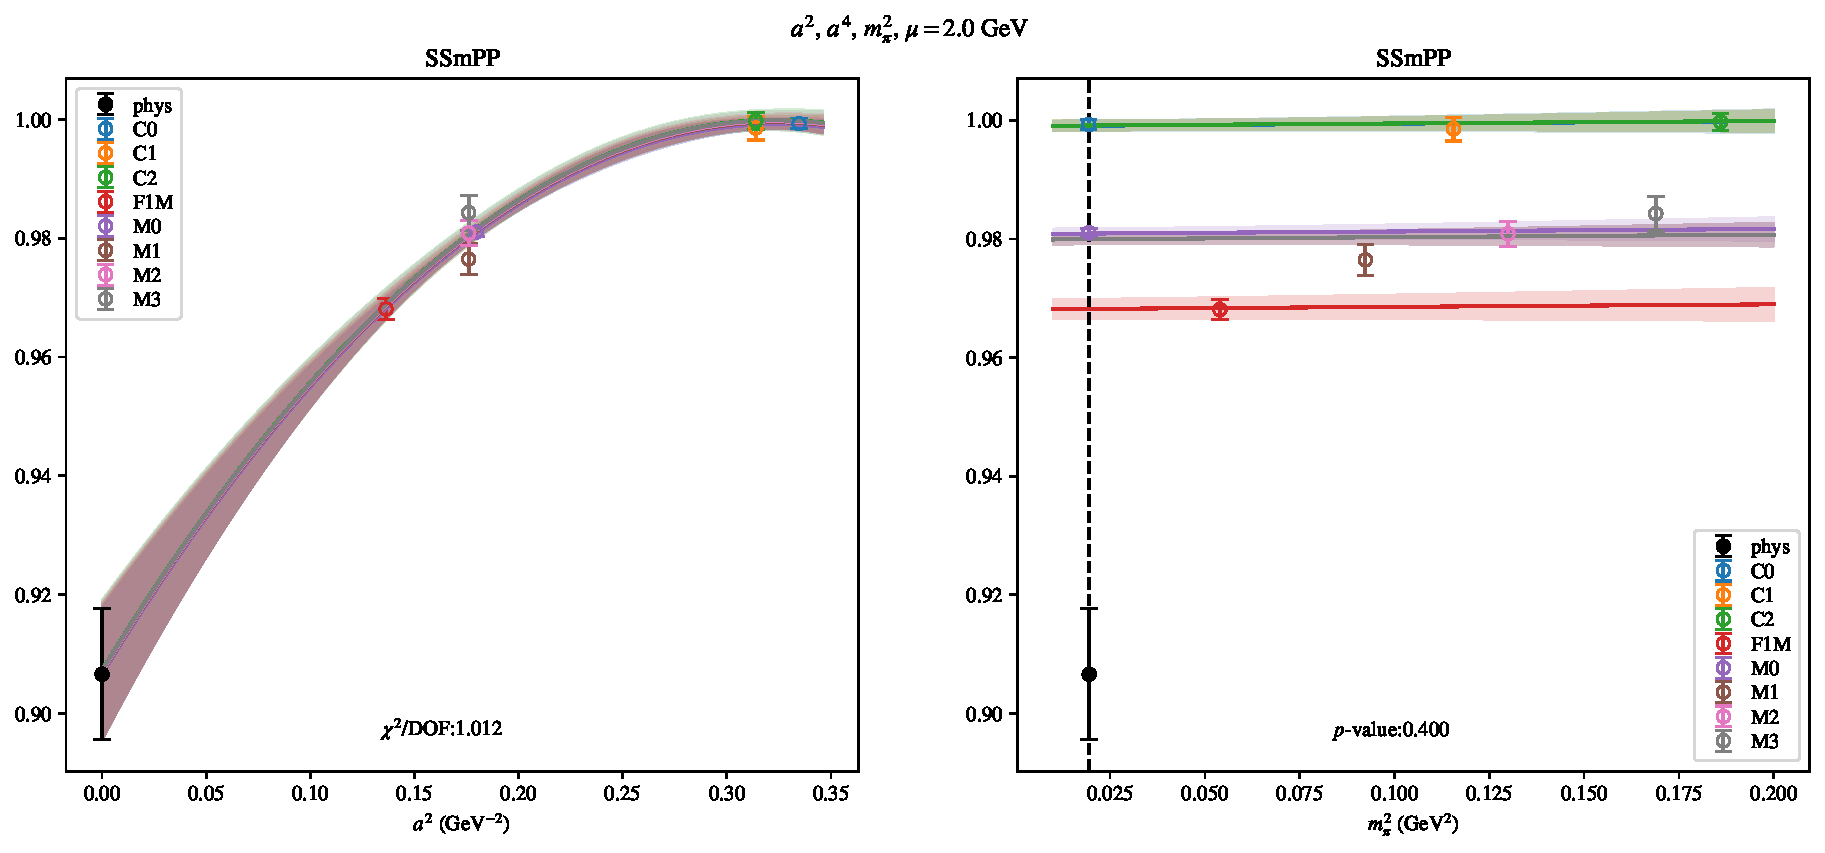
\includepdf[link, pages=-]{SSmPP/a2a4m2_20.pdf}
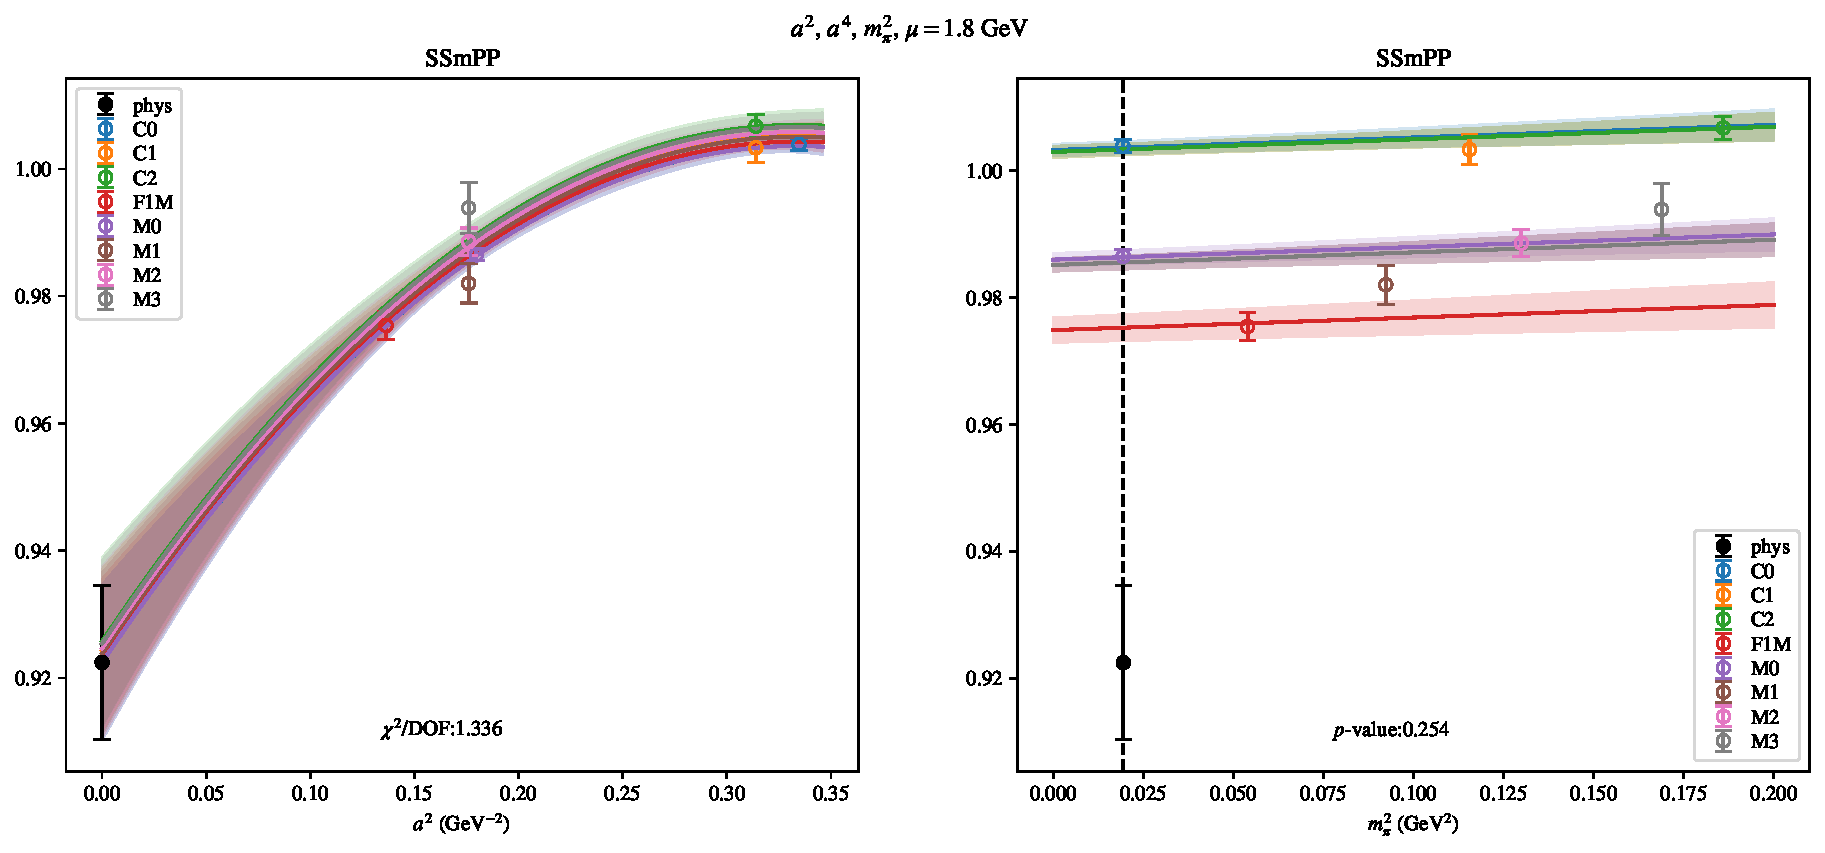
\includepdf[link, pages=-]{SSmPP/a2a4m2_18.pdf}
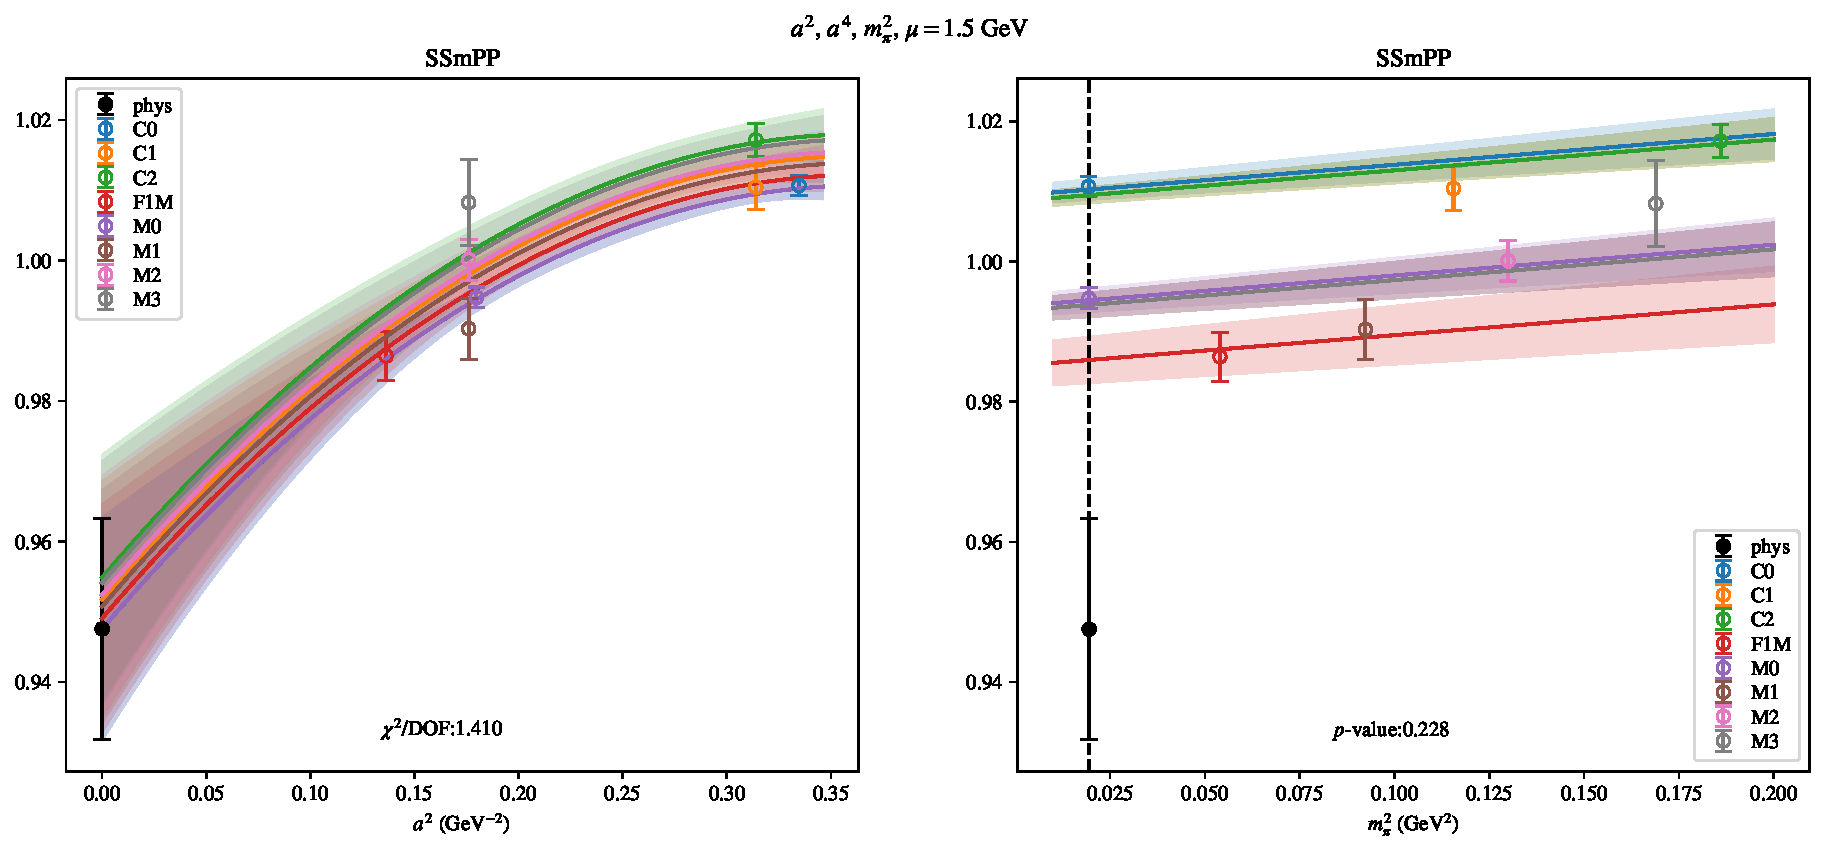
\includepdf[link, pages=-]{SSmPP/a2a4m2_15.pdf}
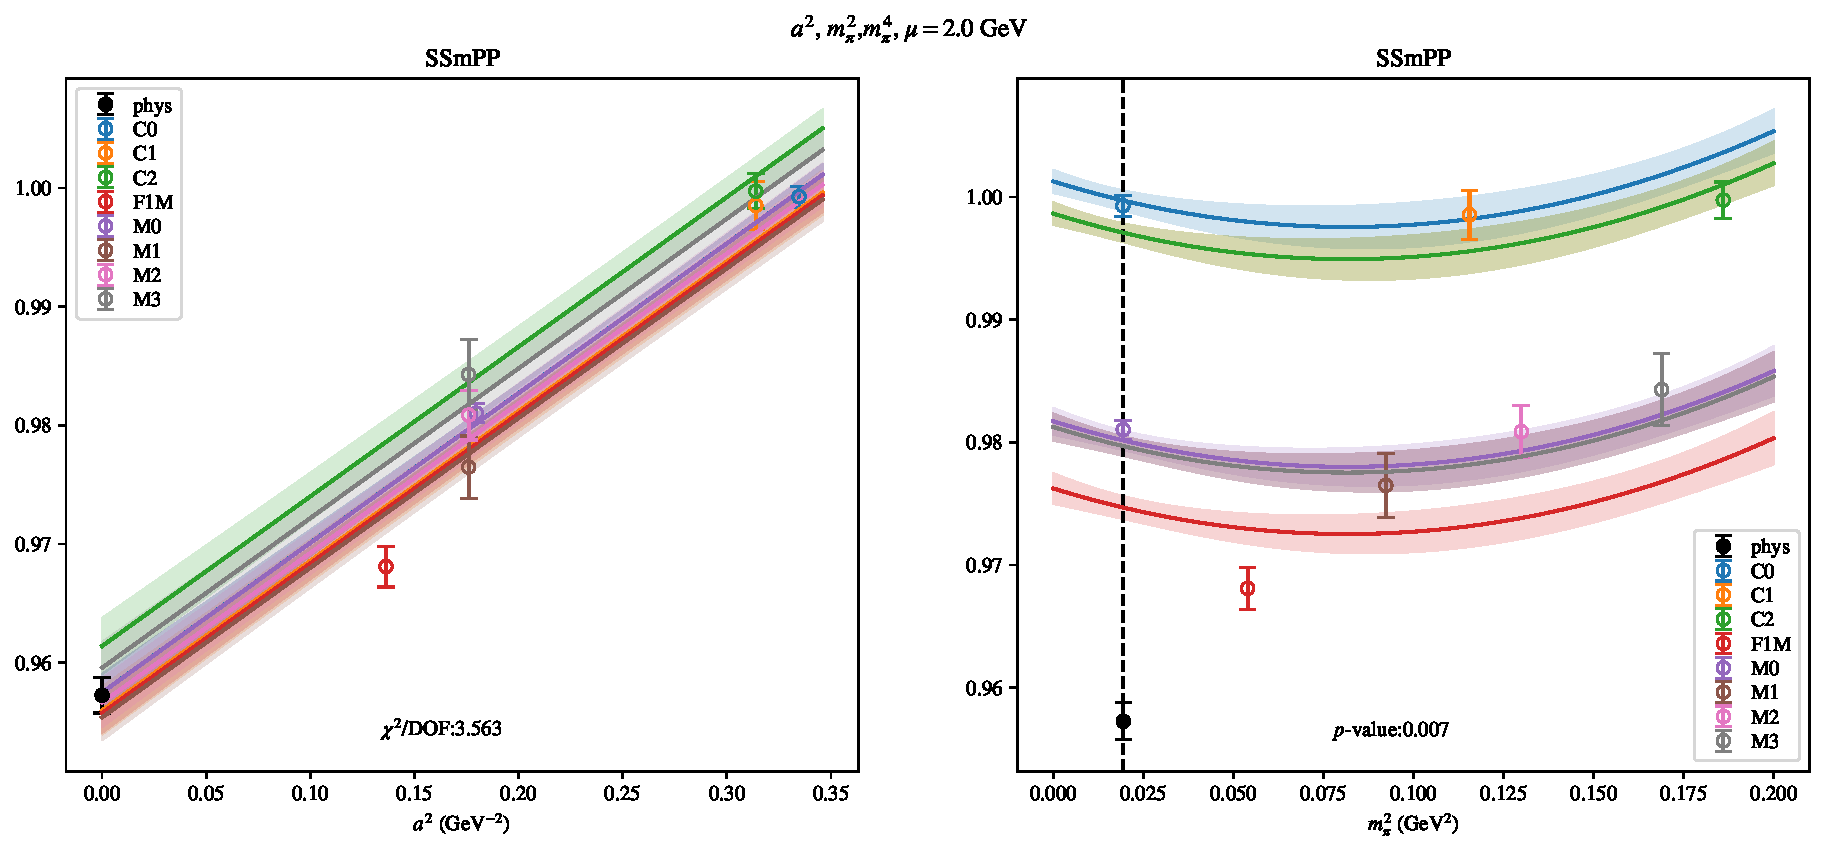
\includepdf[link, pages=-]{SSmPP/a2m2m4_20.pdf}
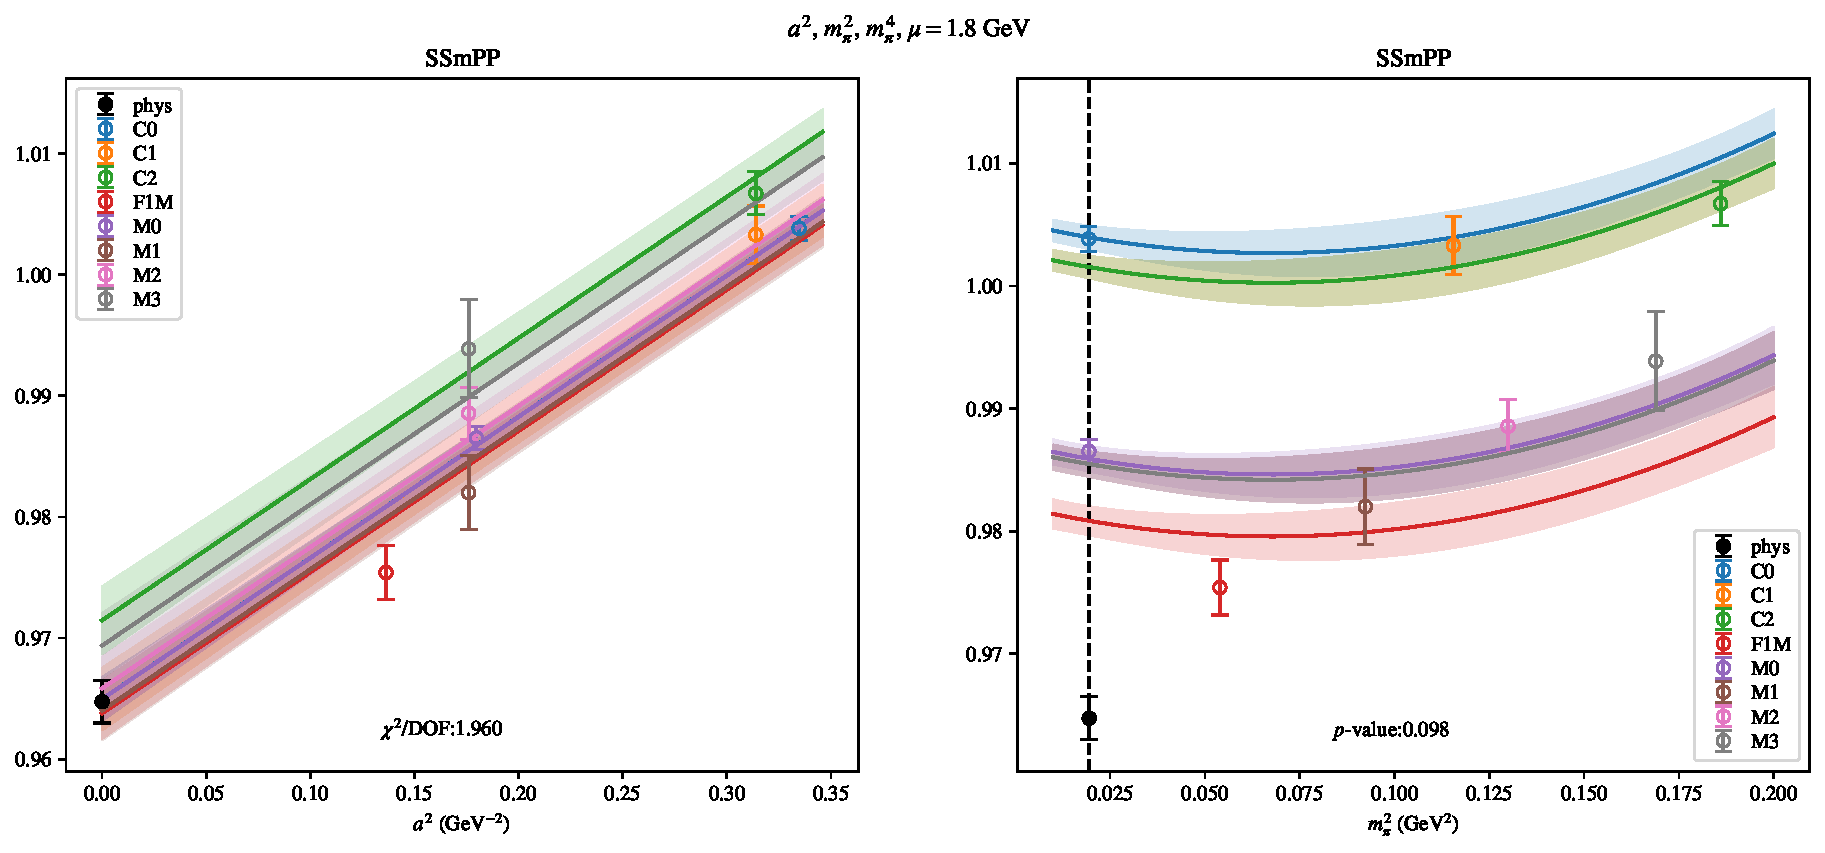
\includepdf[link, pages=-]{SSmPP/a2m2m4_18.pdf}
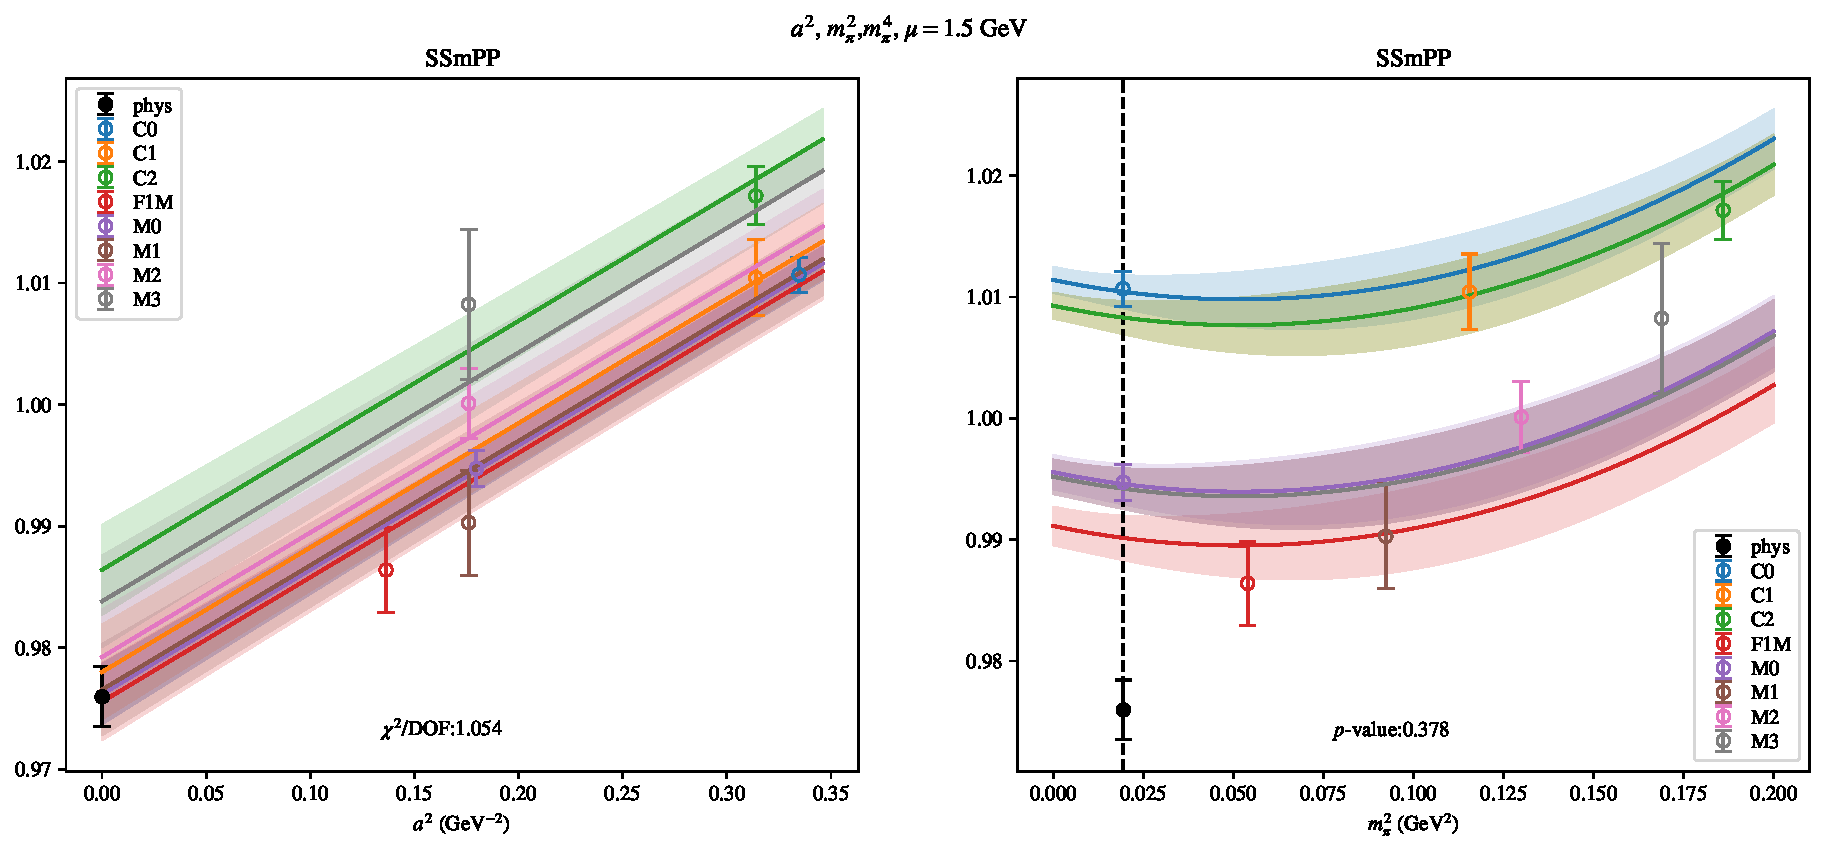
\includepdf[link, pages=-]{SSmPP/a2m2m4_15.pdf}
\clearpage
\section{SSpPP}
\begin{table}[!h]
\begin{center}
\begin{tabular*}{\linewidth}{@{\extracolsep{\fill}} |c|c|c|c|c|}
\hline
$\mu$ (GeV) & $a^2$, $m_\pi^2$ & $a^2$, $m_\pi^2$ no C & $a^2$, $a^4$, $m_\pi^2$ & $a^2$, $m_\pi^2$, $m_\pi^4$\\
\hline
2.0& \hyperlink{SSpPP/a2m2_20.pdf.1}{\textbf{0.56754(98)}: 4.716 (0.0)} & \hyperlink{SSpPP/a2m2noC_20.pdf.1}{\textbf{0.5922(55)}: 0.797 (0.451)} & \hyperlink{SSpPP/a2a4m2_20.pdf.1}{\textbf{0.5969(91)}: 3.427 (0.008)} & \hyperlink{SSpPP/a2m2m4_20.pdf.1}{\textbf{0.5666(10)}: 4.48 (0.001)}\\
1.8& \hyperlink{SSpPP/a2m2_18.pdf.1}{\textbf{0.5840(12)}: 3.149 (0.008)} & \hyperlink{SSpPP/a2m2noC_18.pdf.1}{\textbf{0.6114(59)}: 0.41 (0.664)} & \hyperlink{SSpPP/a2a4m2_18.pdf.1}{\textbf{0.6210(99)}: 1.37 (0.242)} & \hyperlink{SSpPP/a2m2m4_18.pdf.1}{\textbf{0.5832(11)}: 3.371 (0.009)}\\
1.5& \hyperlink{SSpPP/a2m2_15.pdf.1}{\textbf{0.6089(17)}: 1.887 (0.093)} & \hyperlink{SSpPP/a2m2noC_15.pdf.1}{\textbf{0.6400(71)}: 0.233 (0.792)} & \hyperlink{SSpPP/a2a4m2_15.pdf.1}{\textbf{0.657(12)}: 0.272 (0.896)} & \hyperlink{SSpPP/a2m2m4_15.pdf.1}{\textbf{0.6084(15)}: 2.247 (0.061)}\\
\hline
\end{tabular*}
\caption{Physical point value from chiral and continuum extrapolation at renormalisation scale $\mu$. Entries are \textbf{value(error)}: $\chi^2/\text{DOF}$ ($p$-value).}
\end{center}
\end{table}
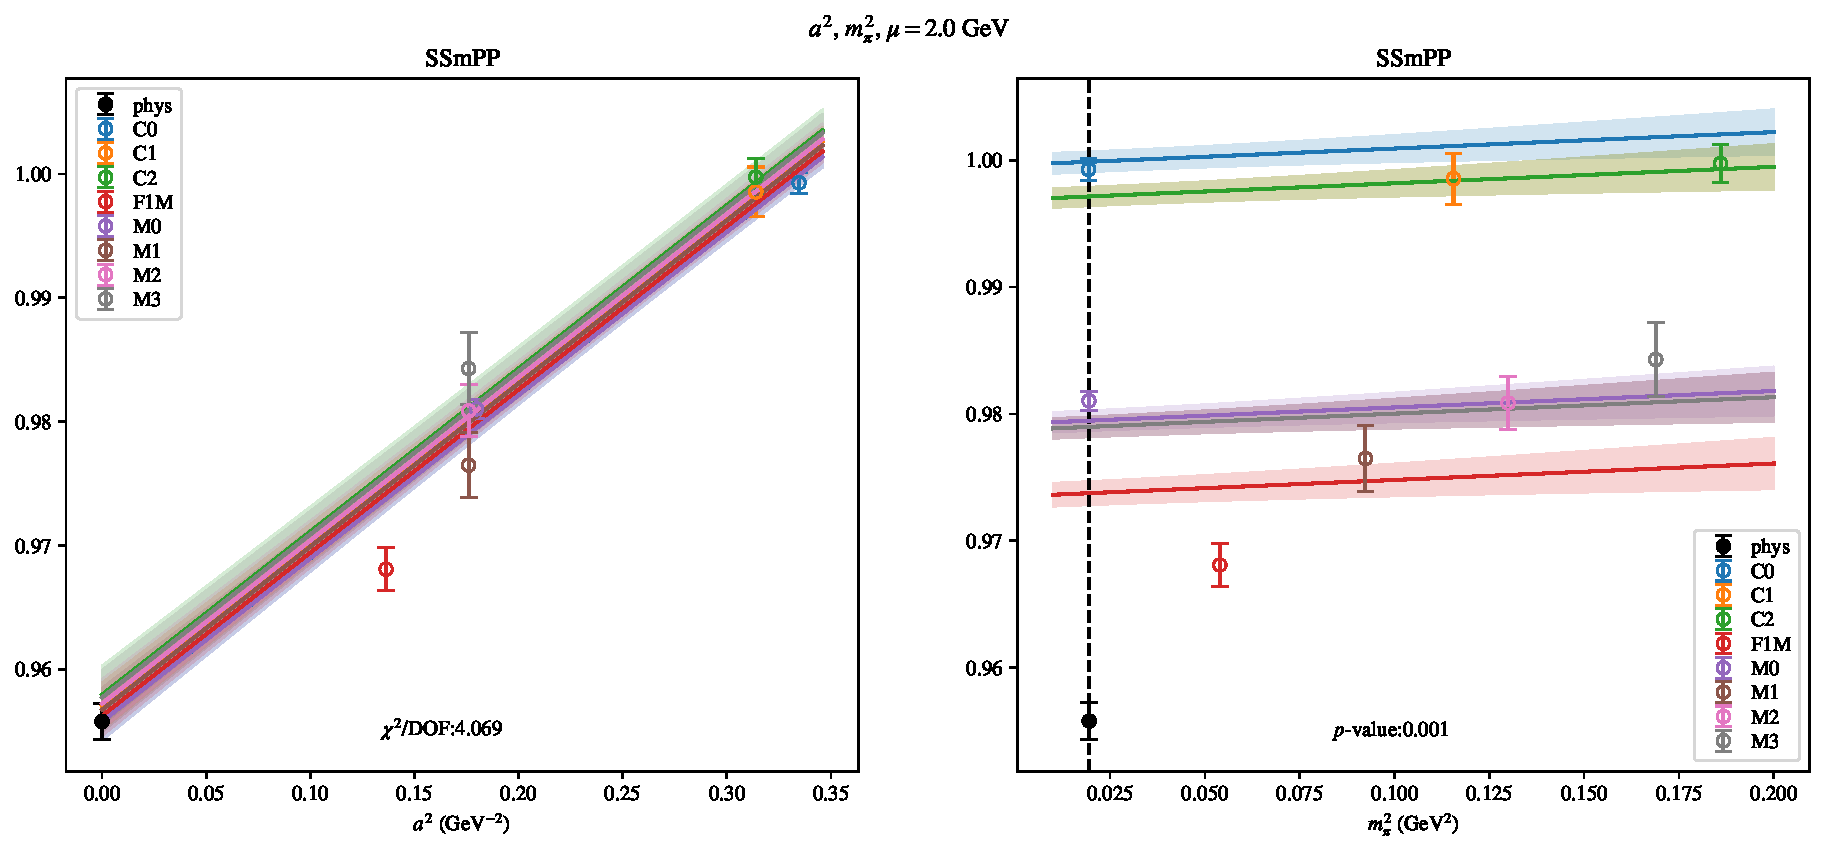
\includepdf[link, pages=-]{SSpPP/a2m2_20.pdf}
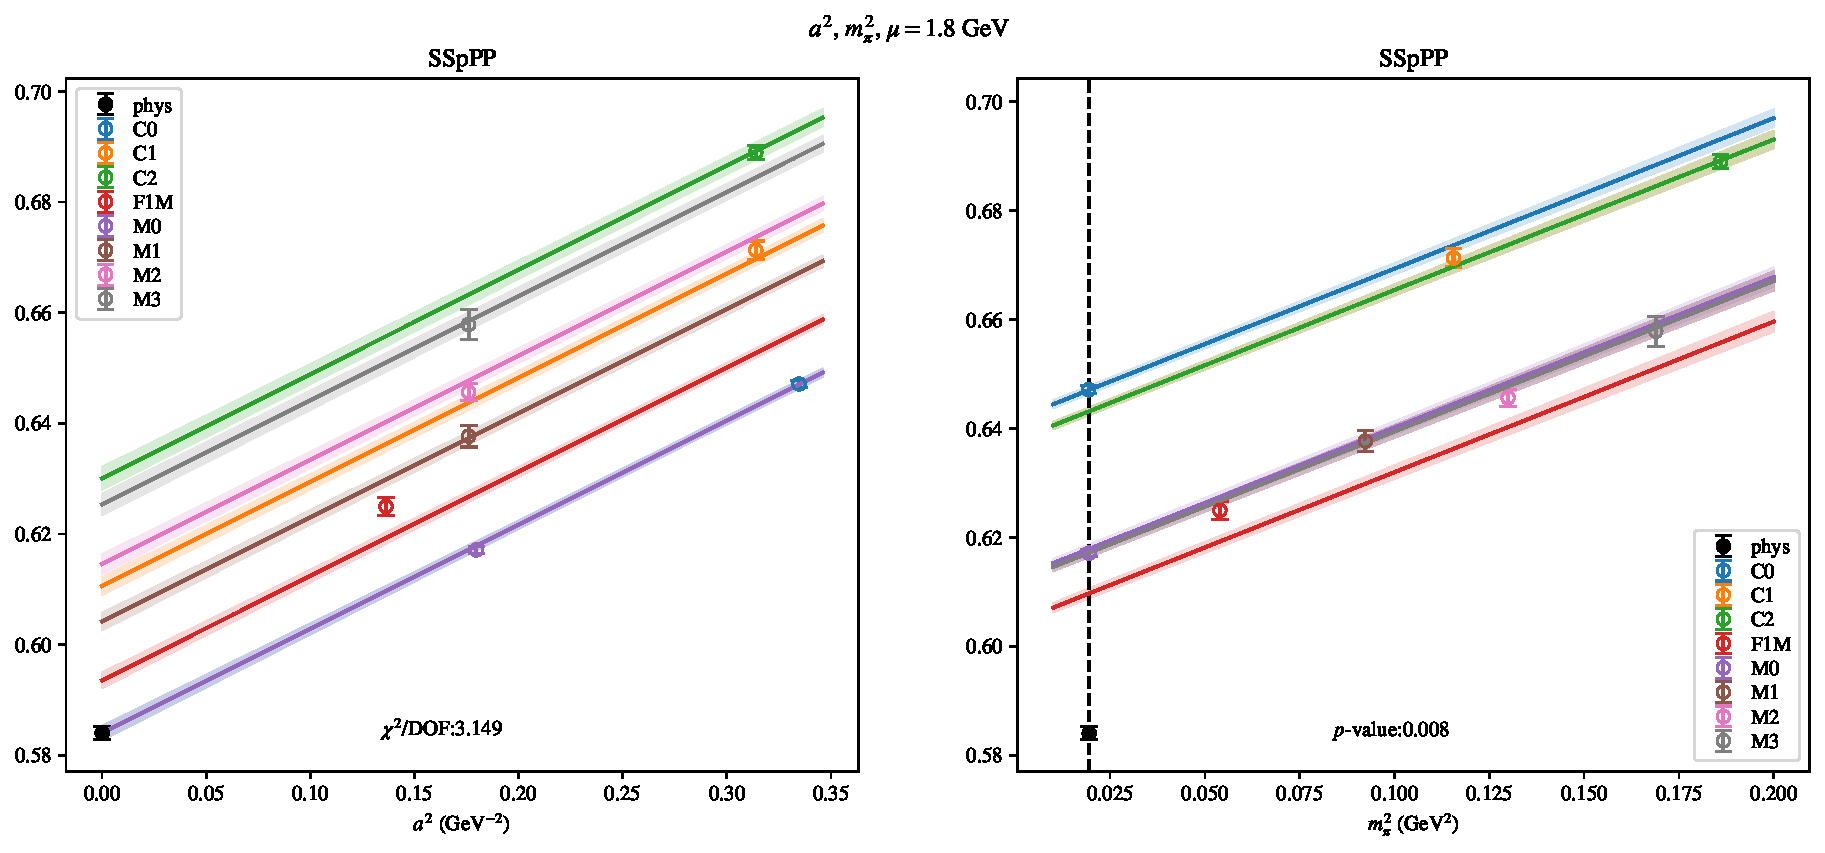
\includepdf[link, pages=-]{SSpPP/a2m2_18.pdf}
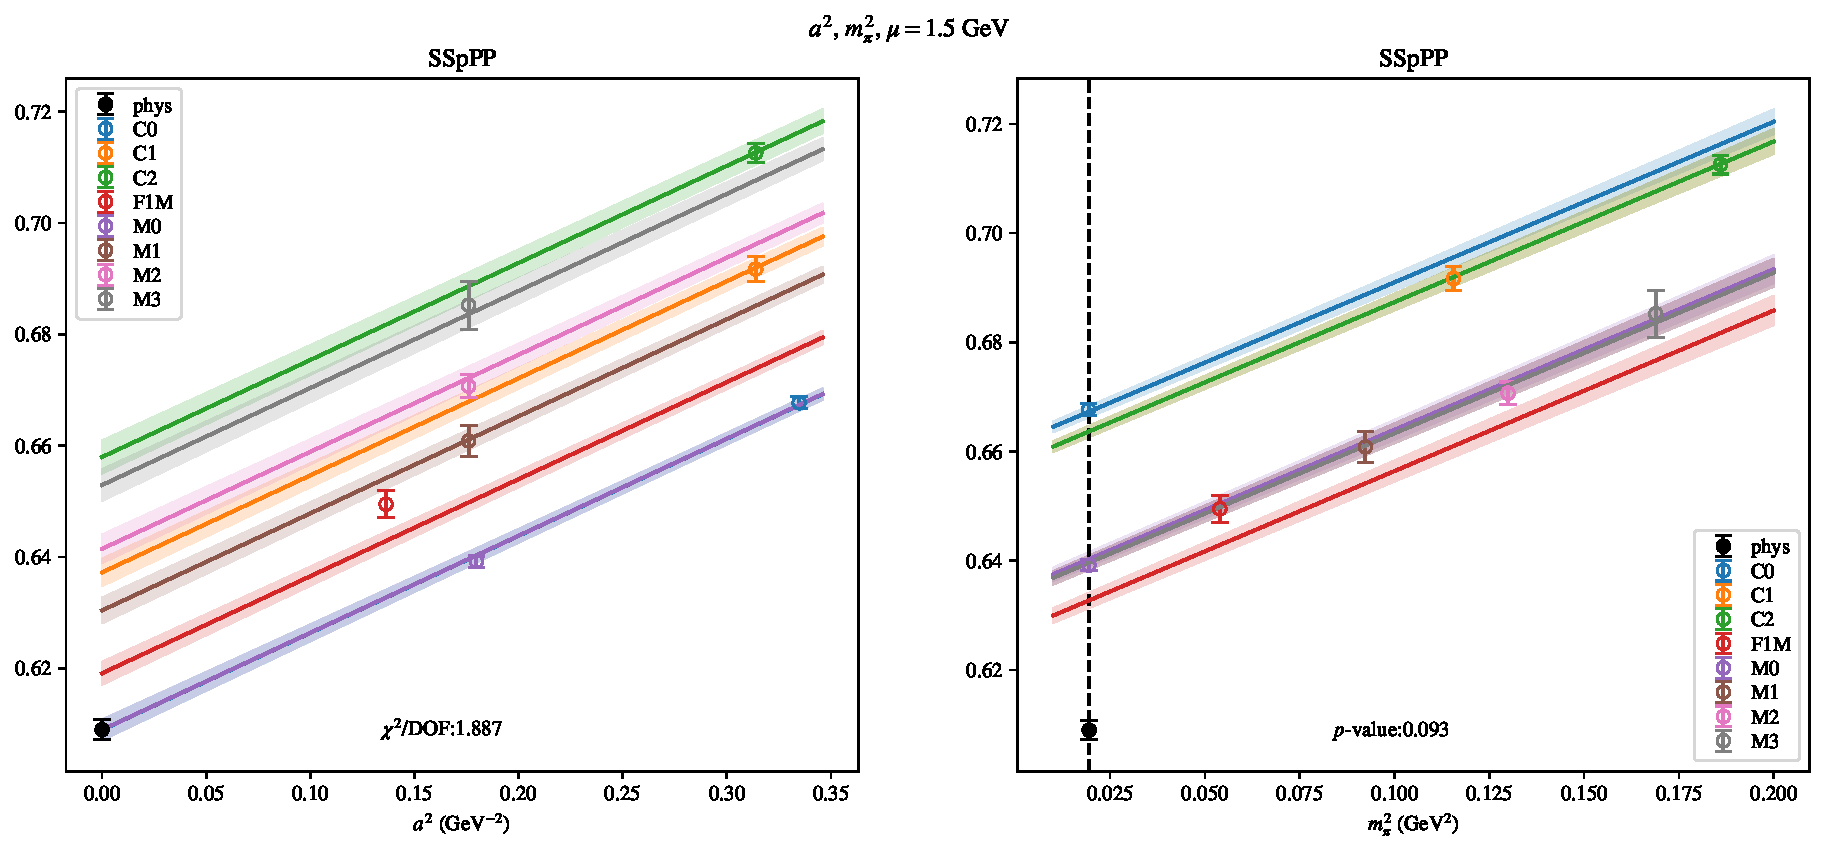
\includepdf[link, pages=-]{SSpPP/a2m2_15.pdf}
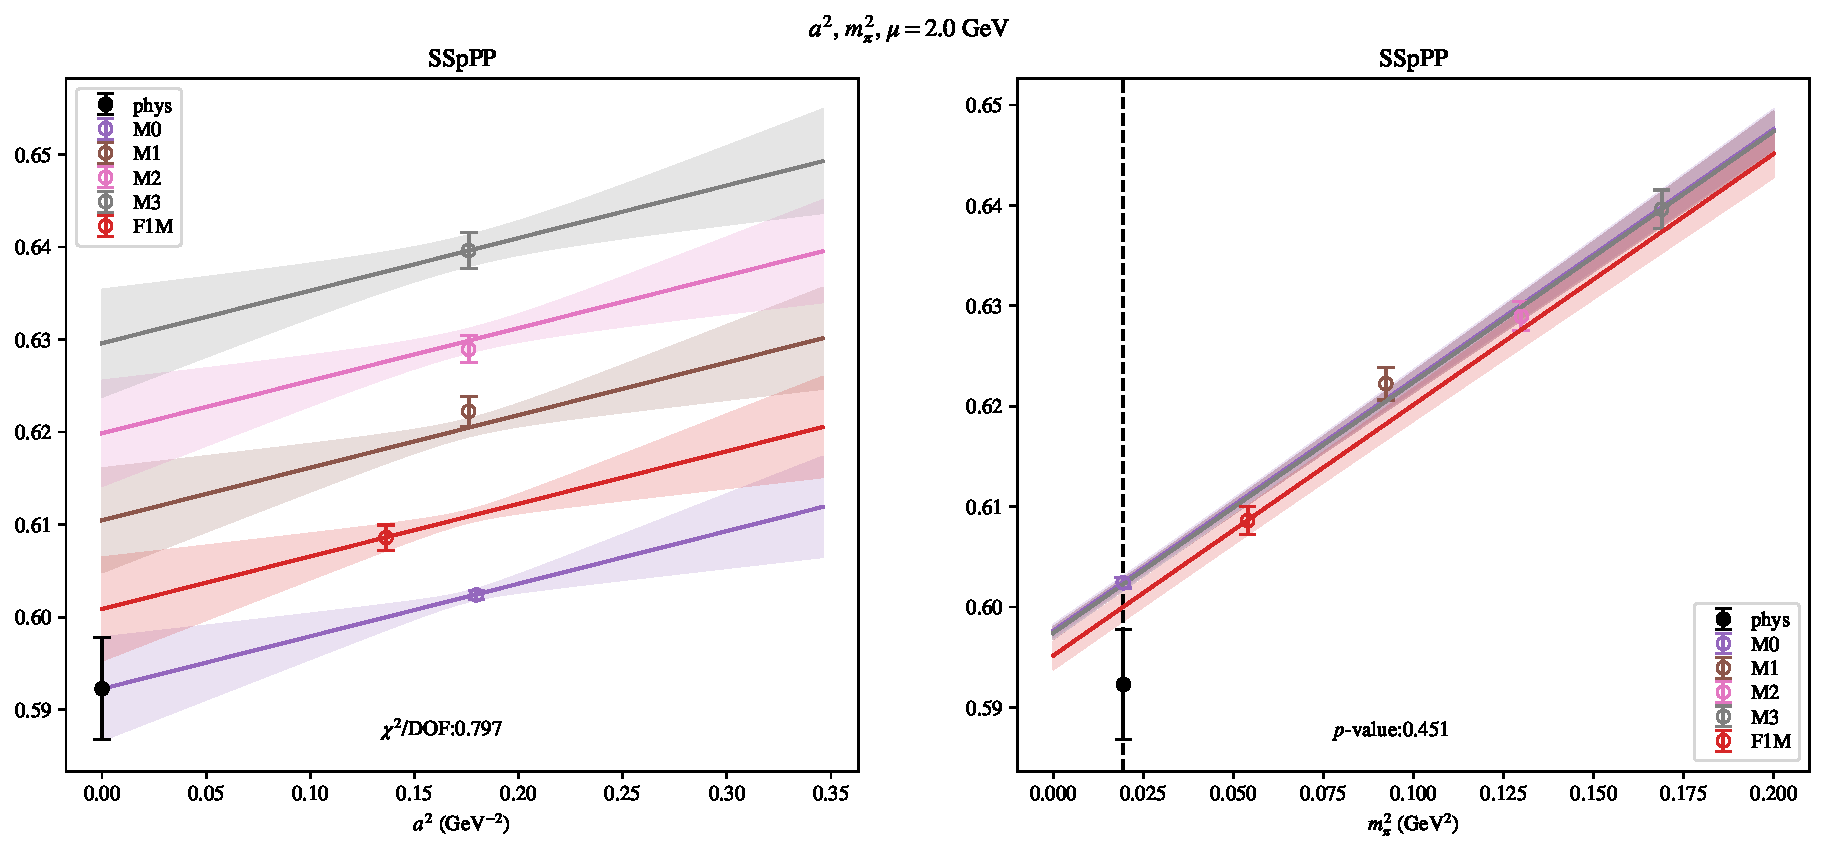
\includepdf[link, pages=-]{SSpPP/a2m2noC_20.pdf}
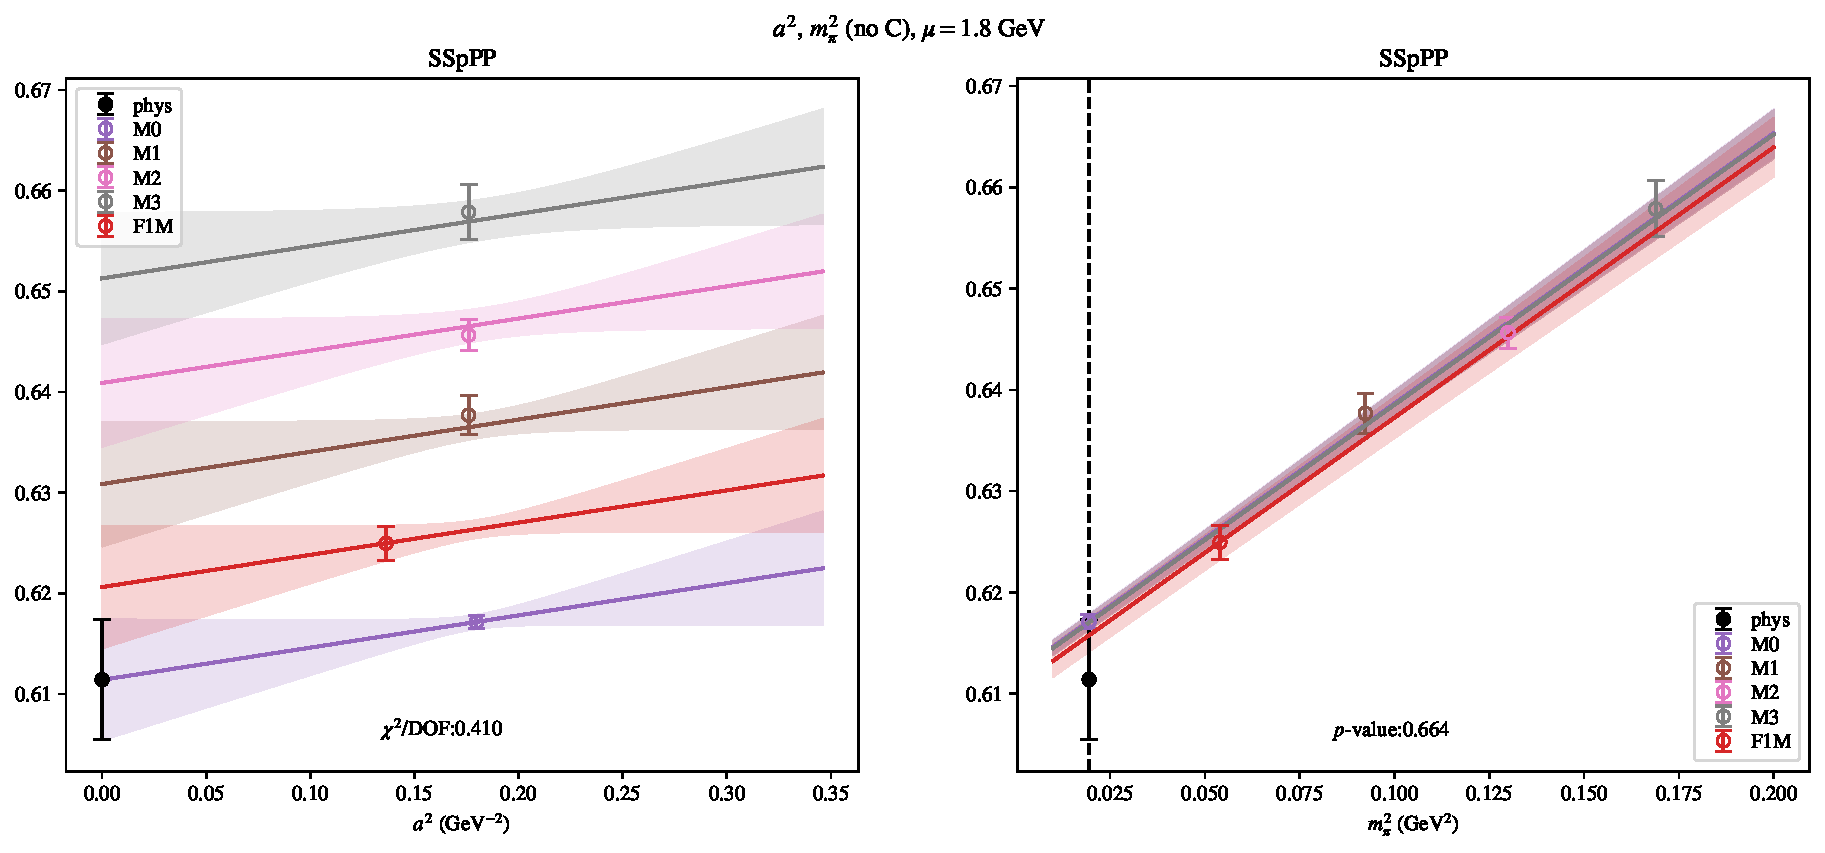
\includepdf[link, pages=-]{SSpPP/a2m2noC_18.pdf}
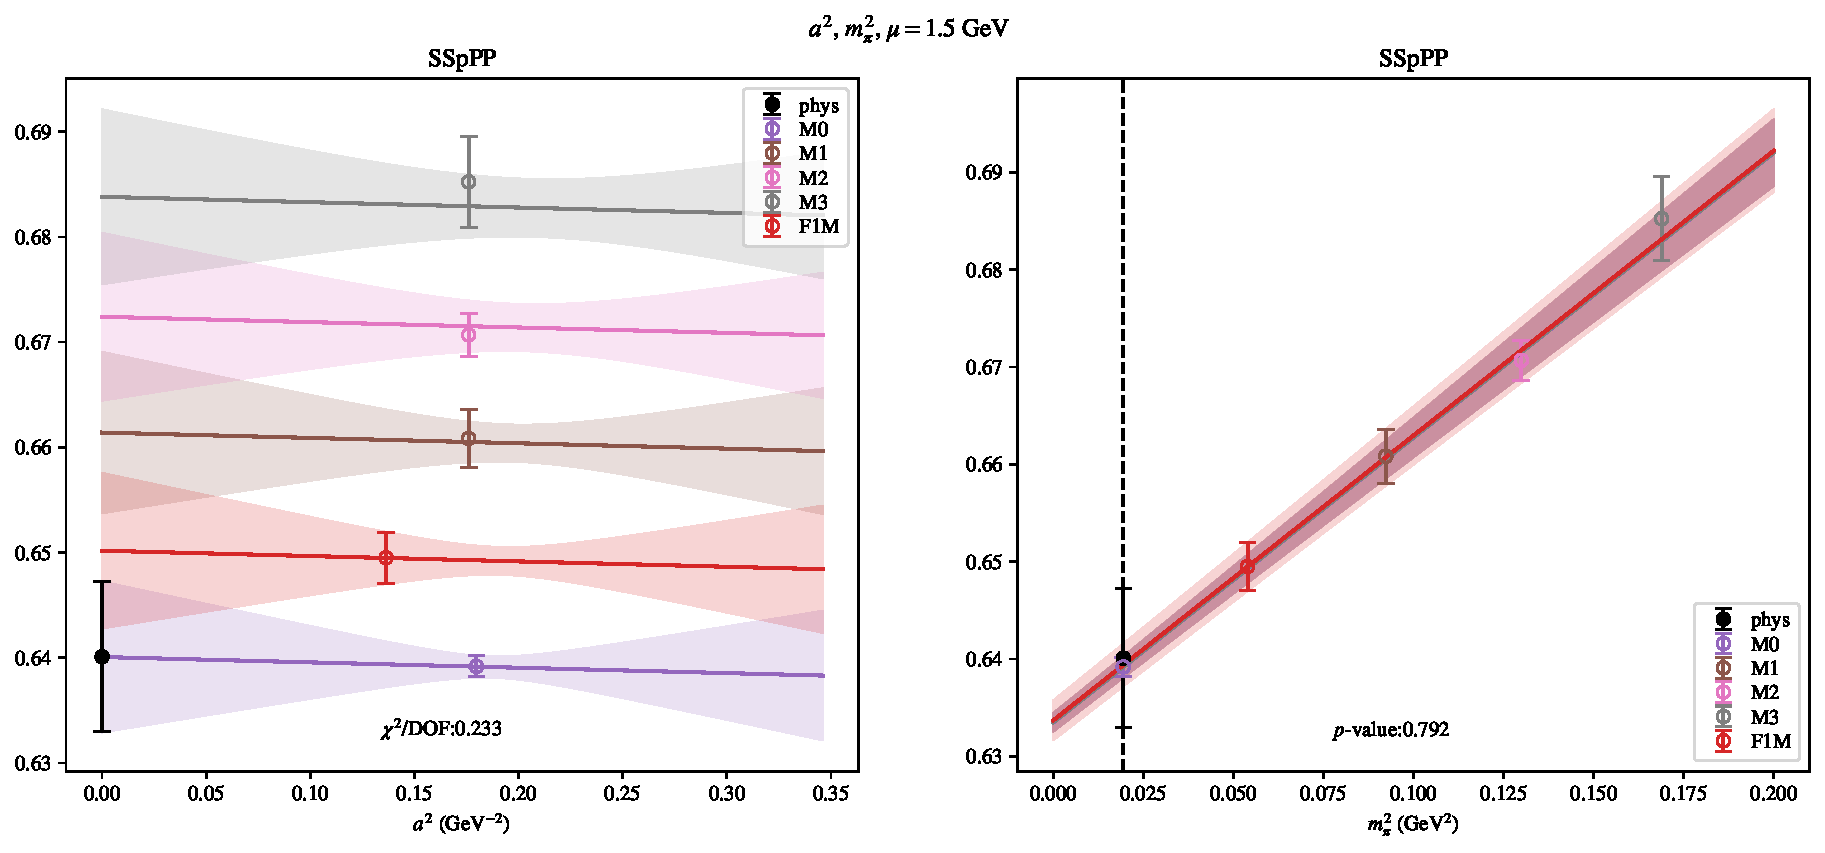
\includepdf[link, pages=-]{SSpPP/a2m2noC_15.pdf}
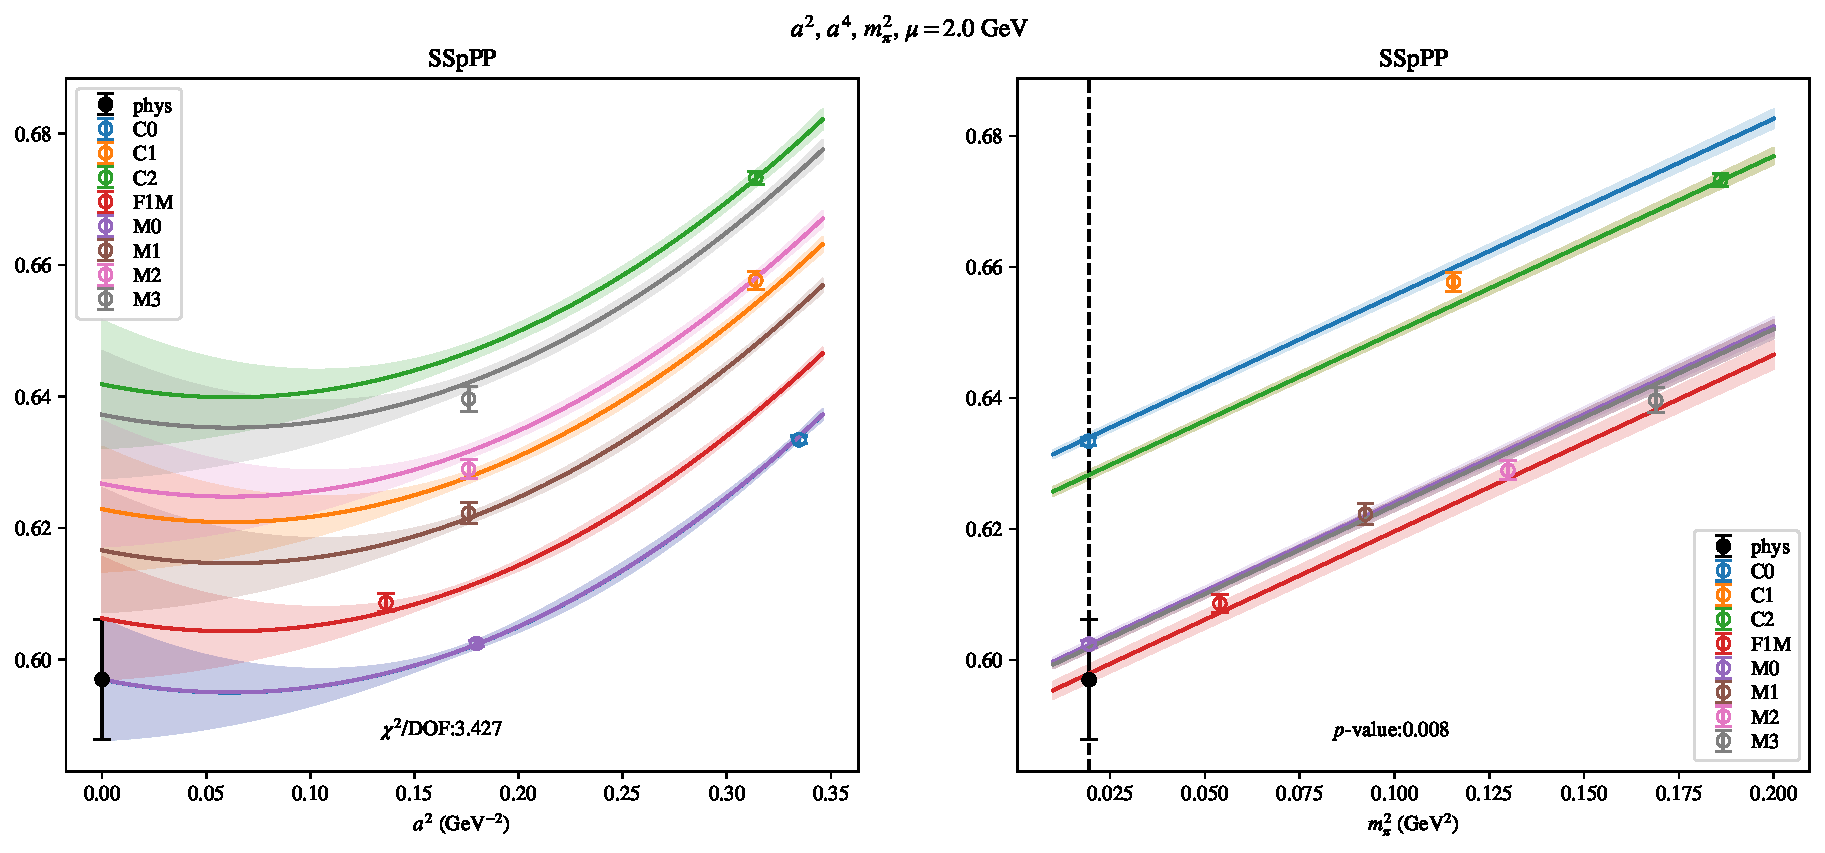
\includepdf[link, pages=-]{SSpPP/a2a4m2_20.pdf}
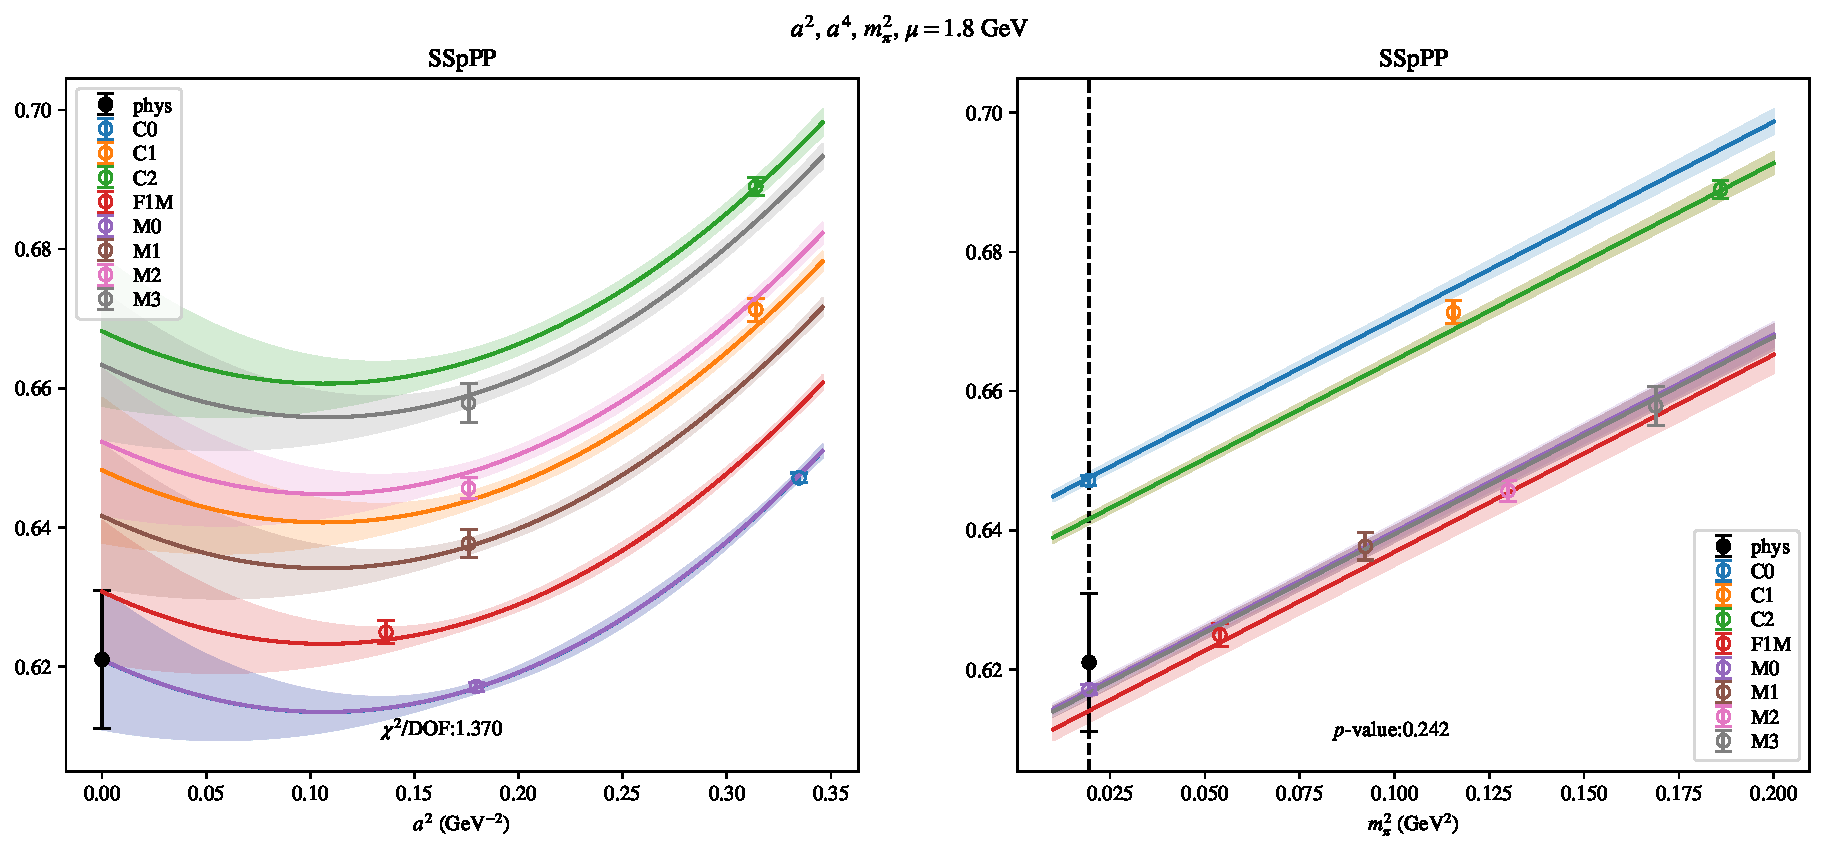
\includepdf[link, pages=-]{SSpPP/a2a4m2_18.pdf}
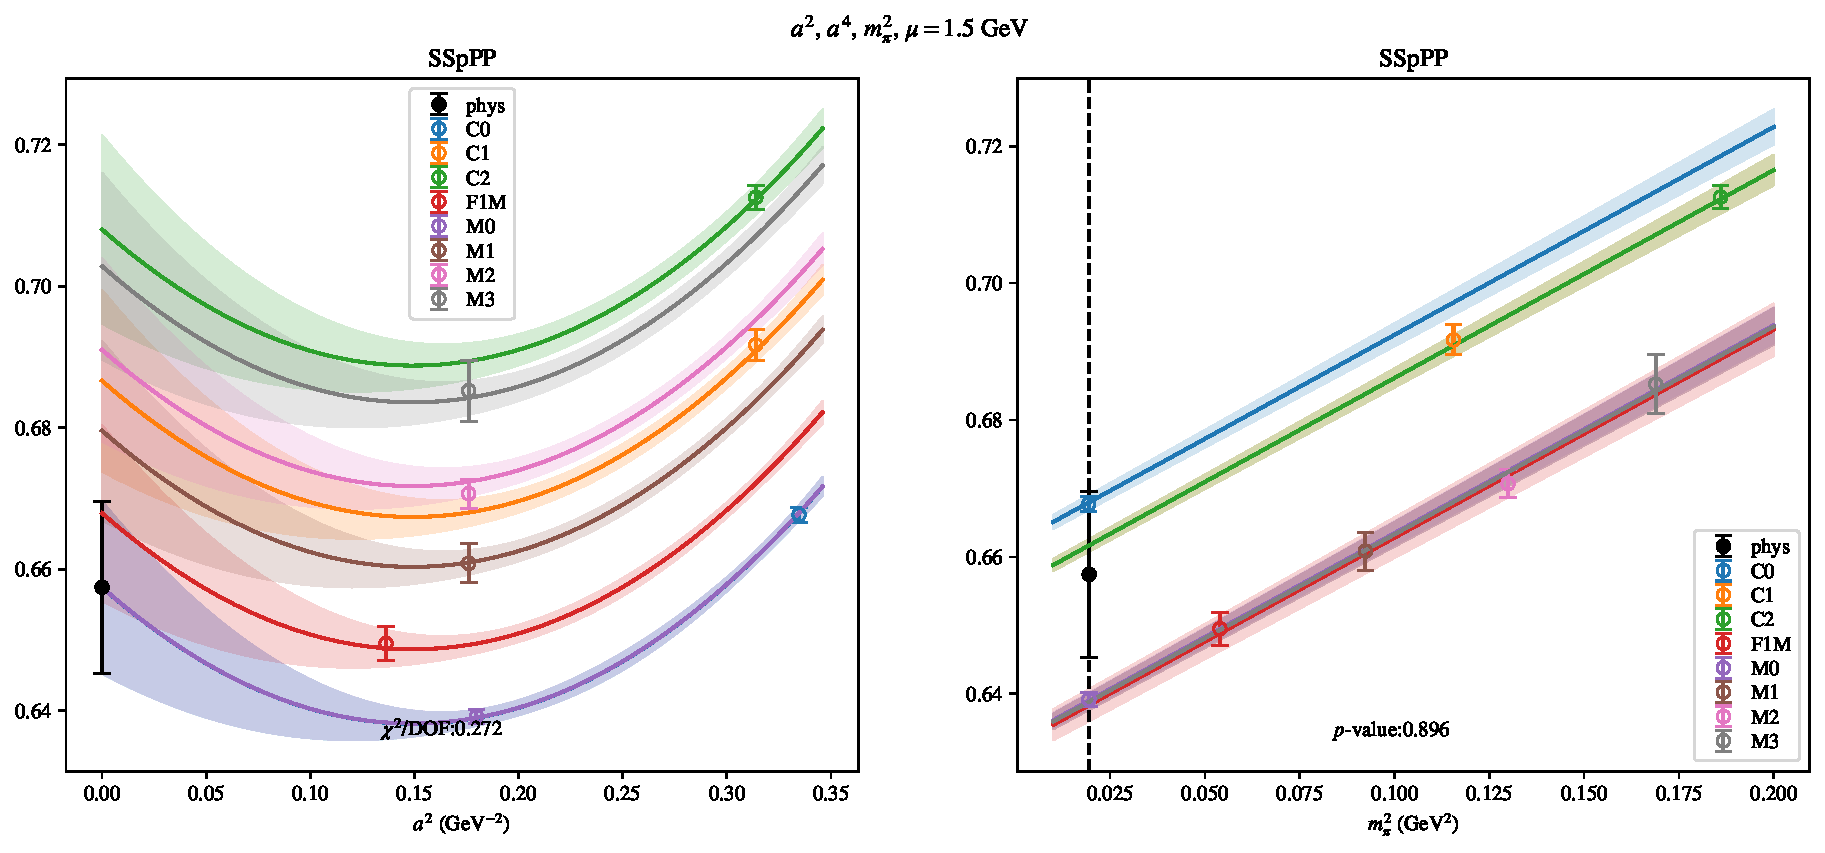
\includepdf[link, pages=-]{SSpPP/a2a4m2_15.pdf}
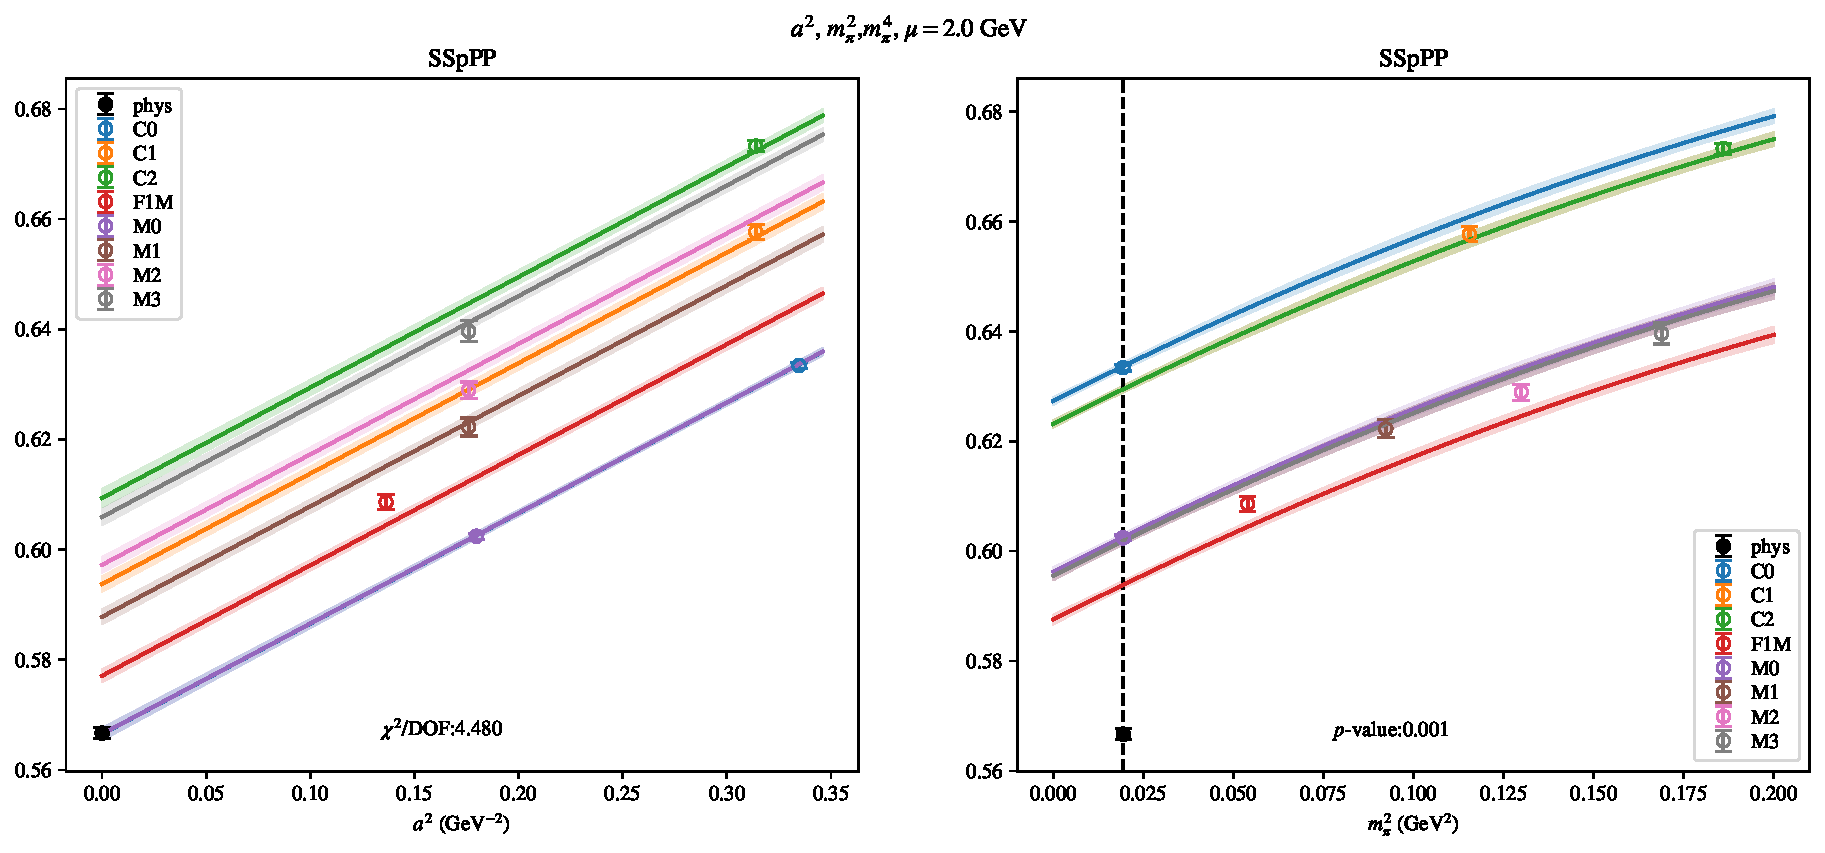
\includepdf[link, pages=-]{SSpPP/a2m2m4_20.pdf}
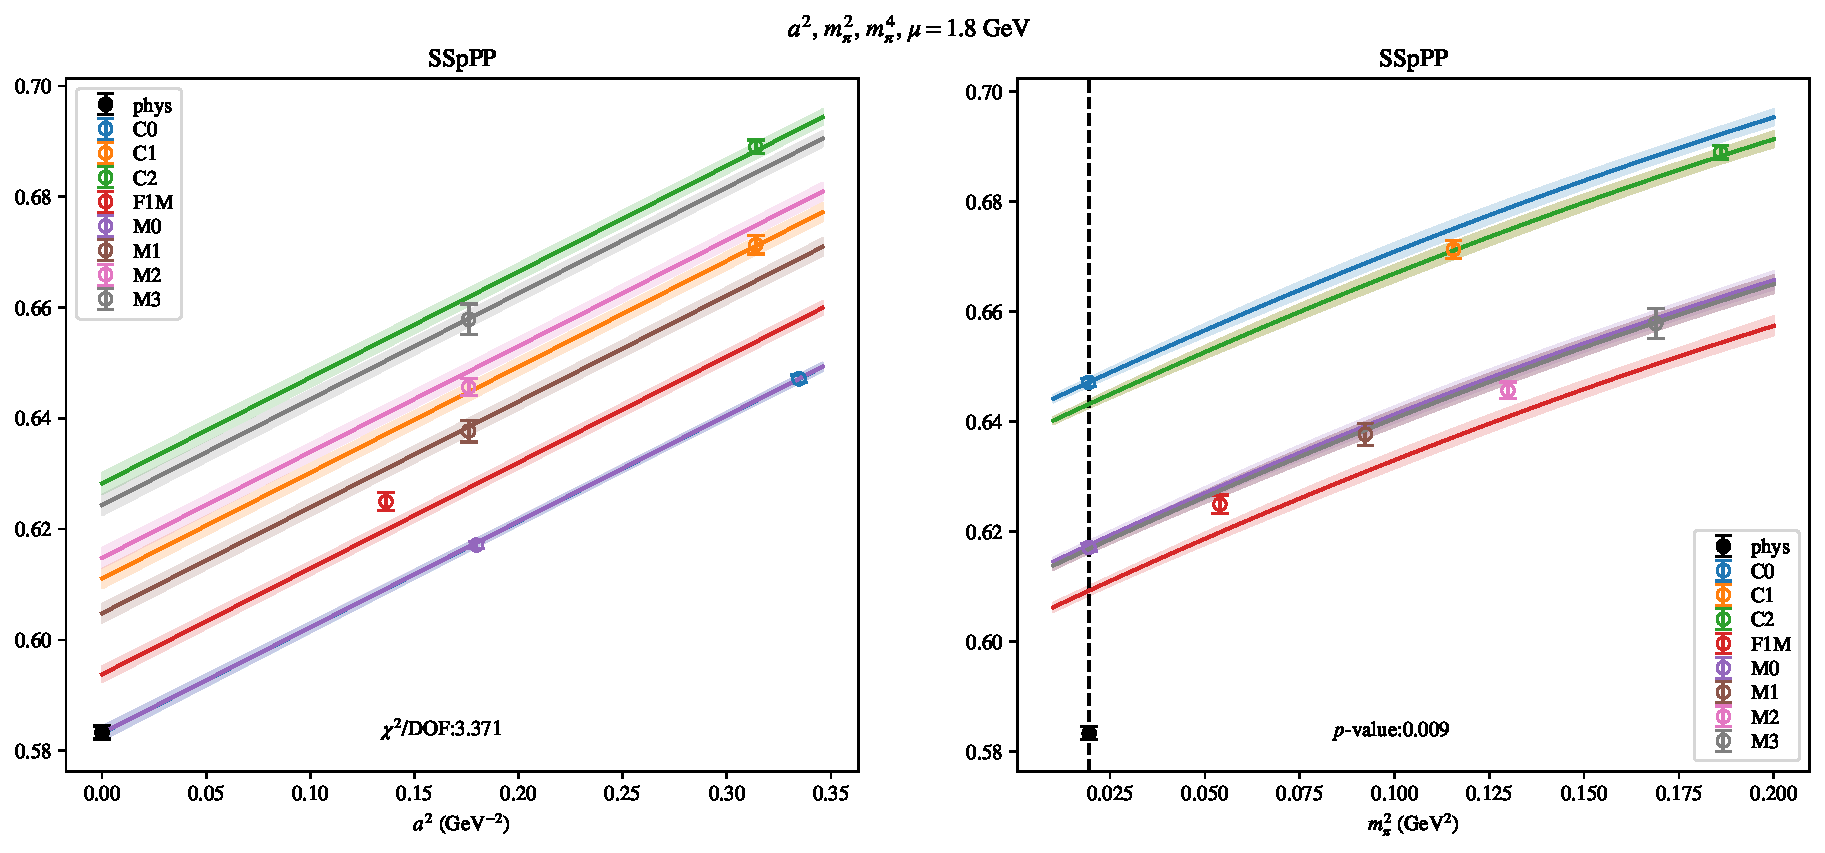
\includepdf[link, pages=-]{SSpPP/a2m2m4_18.pdf}
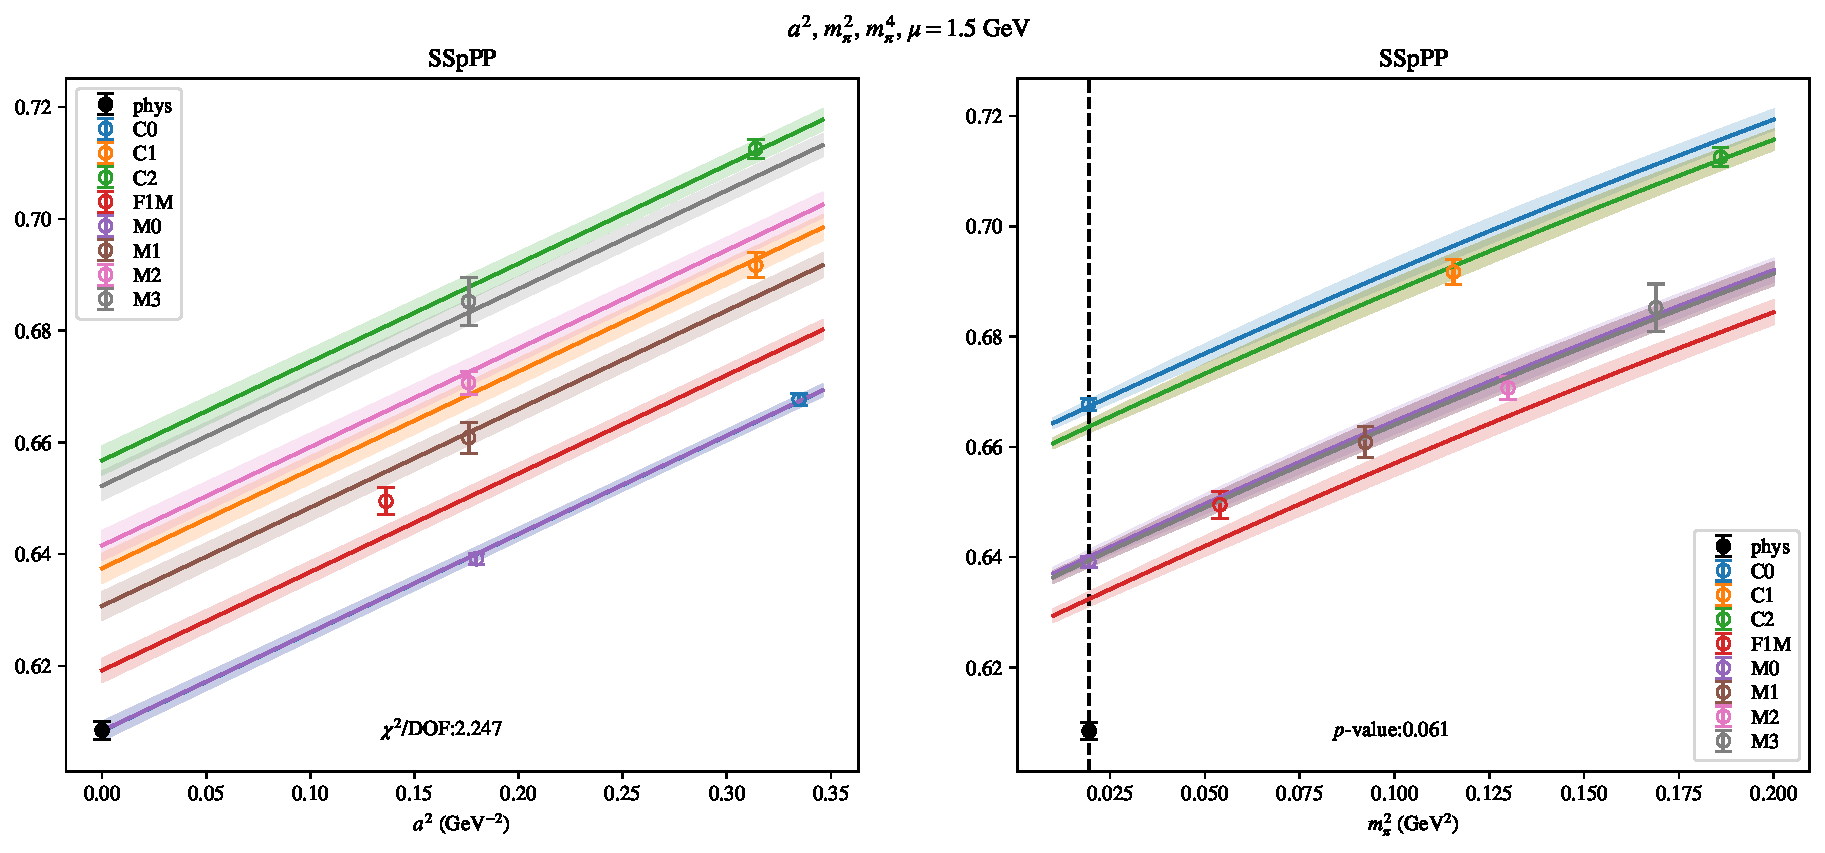
\includepdf[link, pages=-]{SSpPP/a2m2m4_15.pdf}
\clearpage
\section{TT}
\begin{table}[!h]
\begin{center}
\begin{tabular*}{\linewidth}{@{\extracolsep{\fill}} |c|c|c|c|c|}
\hline
$\mu$ (GeV) & $a^2$, $m_\pi^2$ & $a^2$, $m_\pi^2$ no C & $a^2$, $a^4$, $m_\pi^2$ & $a^2$, $m_\pi^2$, $m_\pi^4$\\
\hline
2.0& \hyperlink{TT/a2m2_20.pdf.1}{\textbf{0.5940(10)}: 7.141 (0.0)} & \hyperlink{TT/a2m2noC_20.pdf.1}{\textbf{0.6355(60)}: 0.563 (0.569)} & \hyperlink{TT/a2a4m2_20.pdf.1}{\textbf{0.658(10)}: 1.281 (0.275)} & \hyperlink{TT/a2m2m4_20.pdf.1}{\textbf{0.5930(10)}: 6.036 (0.0)}\\
1.8& \hyperlink{TT/a2m2_18.pdf.1}{\textbf{0.6358(17)}: 3.741 (0.002)} & \hyperlink{TT/a2m2noC_18.pdf.1}{\textbf{0.6796(79)}: 0.363 (0.695)} & \hyperlink{TT/a2a4m2_18.pdf.1}{\textbf{0.711(13)}: 0.386 (0.819)} & \hyperlink{TT/a2m2m4_18.pdf.1}{\textbf{0.6345(15)}: 3.542 (0.007)}\\
1.5& \hyperlink{TT/a2m2_15.pdf.1}{\textbf{0.6990(32)}: 2.017 (0.073)} & \hyperlink{TT/a2m2noC_15.pdf.1}{\textbf{0.745(12)}: 0.194 (0.823)} & \hyperlink{TT/a2a4m2_15.pdf.1}{\textbf{0.791(20)}: 0.255 (0.907)} & \hyperlink{TT/a2m2m4_15.pdf.1}{\textbf{0.6975(26)}: 2.13 (0.074)}\\
\hline
\end{tabular*}
\caption{Physical point value from chiral and continuum extrapolation at renormalisation scale $\mu$. Entries are \textbf{value(error)}: $\chi^2/\text{DOF}$ ($p$-value).}
\end{center}
\end{table}
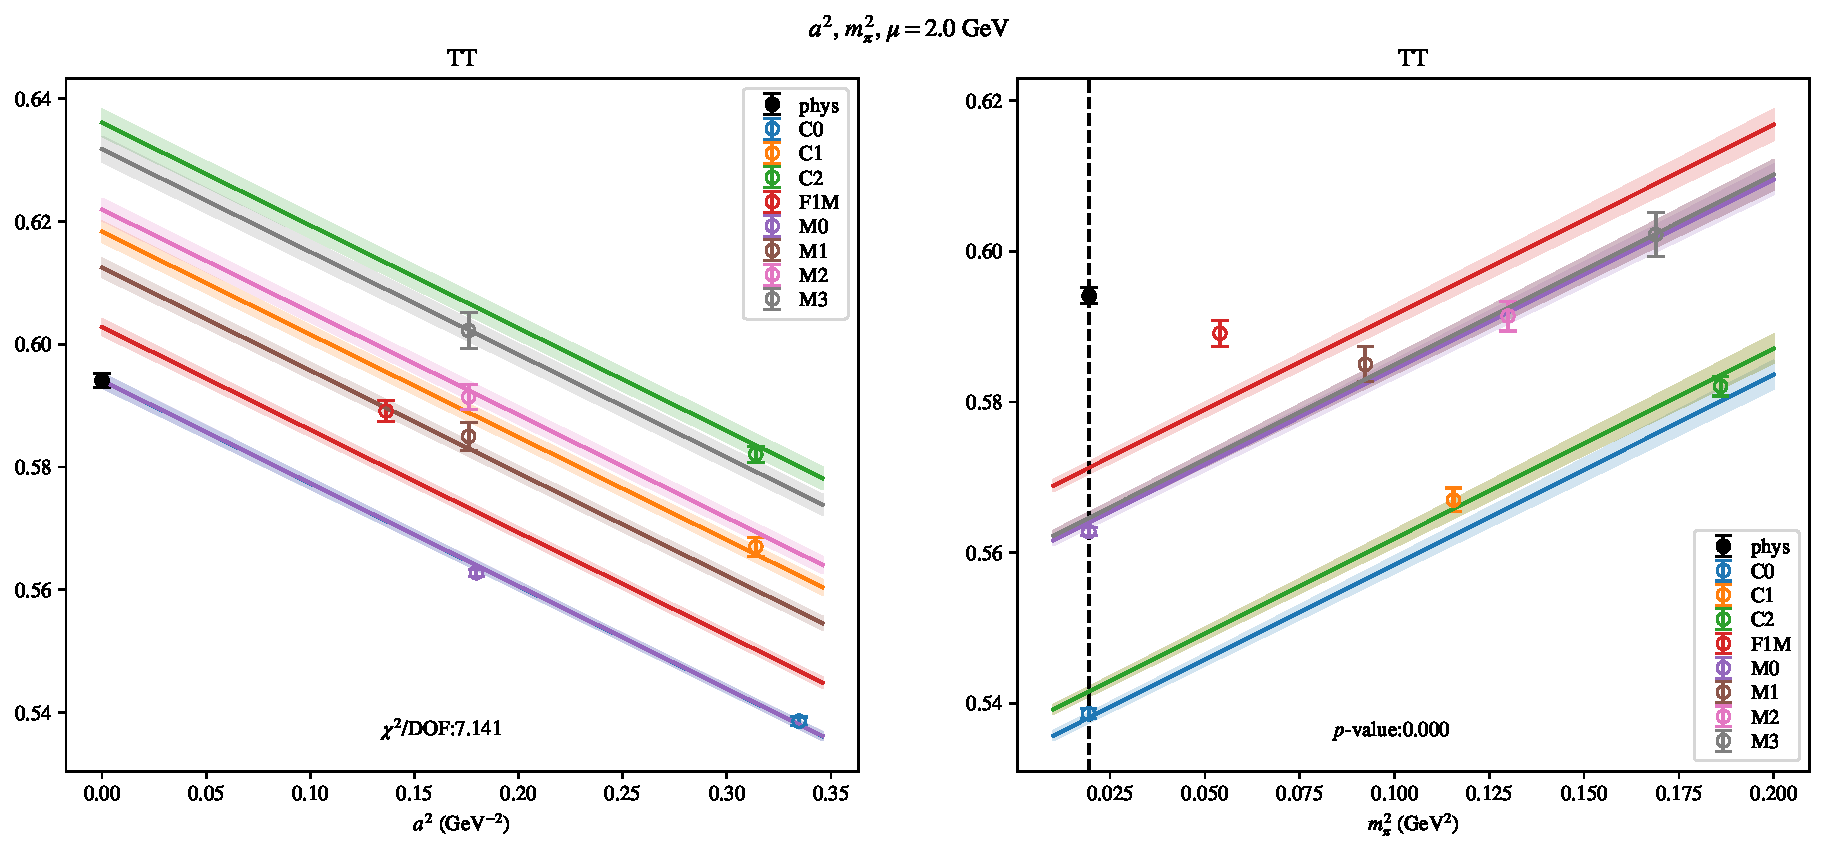
\includepdf[link, pages=-]{TT/a2m2_20.pdf}
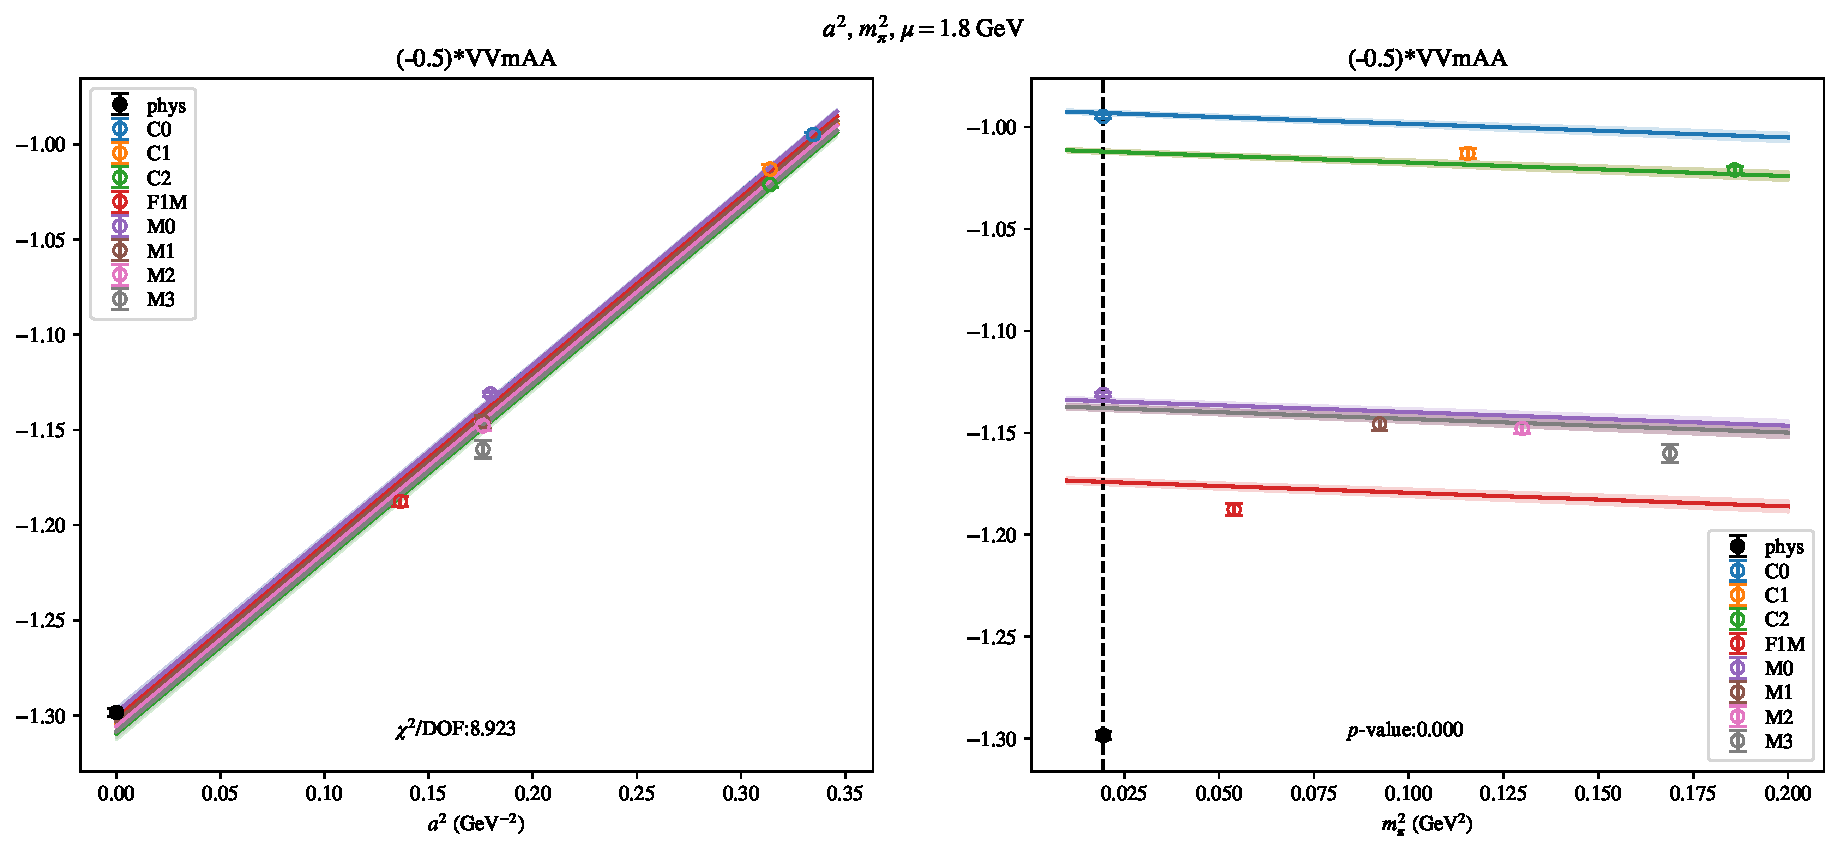
\includepdf[link, pages=-]{TT/a2m2_18.pdf}
\includepdf[link, pages=-]{TT/a2m2_15.pdf}
\includepdf[link, pages=-]{TT/a2m2noC_20.pdf}
\includepdf[link, pages=-]{TT/a2m2noC_18.pdf}
\includepdf[link, pages=-]{TT/a2m2noC_15.pdf}
\includepdf[link, pages=-]{TT/a2a4m2_20.pdf}
\includepdf[link, pages=-]{TT/a2a4m2_18.pdf}
\includepdf[link, pages=-]{TT/a2a4m2_15.pdf}
\includepdf[link, pages=-]{TT/a2m2m4_20.pdf}
\includepdf[link, pages=-]{TT/a2m2m4_18.pdf}
\includepdf[link, pages=-]{TT/a2m2m4_15.pdf}
\end{document}